\documentclass[a4paper]{book}
\usepackage{a4wide}
\usepackage{makeidx}
\usepackage{graphicx}
\usepackage{multicol}
\usepackage{float}
\usepackage{listings}
\usepackage{color}
\usepackage{textcomp}
\usepackage{alltt}
\usepackage{times}
\usepackage{ifpdf}
\ifpdf
\usepackage[pdftex,
            pagebackref=true,
            colorlinks=true,
            linkcolor=blue,
            unicode
           ]{hyperref}
\else
\usepackage[ps2pdf,
            pagebackref=true,
            colorlinks=true,
            linkcolor=blue,
            unicode
           ]{hyperref}
\usepackage{pspicture}
\fi
\usepackage[utf8]{inputenc}
\usepackage{doxygen}
\lstset{language=C++,inputencoding=utf8,basicstyle=\footnotesize,breaklines=true,breakatwhitespace=true,tabsize=8,numbers=left }
\makeindex
\setcounter{tocdepth}{3}
\renewcommand{\footrulewidth}{0.4pt}
\begin{document}
\hypersetup{pageanchor=false}
\begin{titlepage}
\vspace*{7cm}
\begin{center}
{\Large FEM Property Assigner \\[1ex]\large 1 }\\
\vspace*{1cm}
{\large Generated by Doxygen 1.7.1-20100728}\\
\vspace*{0.5cm}
{\small Wed Sep 1 2010 08:00:04}\\
\end{center}
\end{titlepage}
\clearemptydoublepage
\pagenumbering{roman}
\tableofcontents
\clearemptydoublepage
\pagenumbering{arabic}
\hypersetup{pageanchor=true}
\chapter{FEM Property Assigner}
\label{index}\hypertarget{index}{}\begin{DoxyVersion}{Version}
1.0 
\end{DoxyVersion}
\begin{DoxyAuthor}{Author}
Andreas Siegrist 
\end{DoxyAuthor}
\begin{DoxyDate}{Date}
2010
\end{DoxyDate}
FEM Property Assigner is a program that assigns tissue properties of CT images to volumetric meshes 
\chapter{Namespace Index}
\section{Namespace List}
Here is a list of all documented namespaces with brief descriptions:\begin{DoxyCompactList}
\item\contentsline{section}{\hyperlink{namespaceassignment}{assignment} (Contains classes that are related to the property assignment )}{\pageref{namespaceassignment}}{}
\item\contentsline{section}{\hyperlink{namespacecommand}{command} (Contains classes for the command line running mode of the application )}{\pageref{namespacecommand}}{}
\item\contentsline{section}{\hyperlink{namespacectimage}{ctimage} (Contains classes for the processing of CT images )}{\pageref{namespacectimage}}{}
\item\contentsline{section}{\hyperlink{namespacegui}{gui} (Contains classes for the graphical user interface mode of the application )}{\pageref{namespacegui}}{}
\item\contentsline{section}{\hyperlink{namespacemesh}{mesh} (Contains classes for mesh import and export )}{\pageref{namespacemesh}}{}
\item\contentsline{section}{\hyperlink{namespacetest}{test} (Contains unit tests )}{\pageref{namespacetest}}{}
\end{DoxyCompactList}

\chapter{Class Index}
\section{Class Hierarchy}
This inheritance list is sorted roughly, but not completely, alphabetically:\begin{DoxyCompactList}
\item \contentsline{section}{assignment::Interpolator3D}{\pageref{classassignment_1_1_interpolator3_d}}{}
\begin{DoxyCompactList}
\item \contentsline{section}{assignment::TricubicInterpolator}{\pageref{classassignment_1_1_tricubic_interpolator}}{}
\item \contentsline{section}{assignment::TrilinearInterpolator}{\pageref{classassignment_1_1_trilinear_interpolator}}{}
\item \contentsline{section}{test::Interpolator3DMock}{\pageref{classtest_1_1_interpolator3_d_mock}}{}
\end{DoxyCompactList}
\item \contentsline{section}{assignment::NodePropertyAssigner}{\pageref{classassignment_1_1_node_property_assigner}}{}
\begin{DoxyCompactList}
\item \contentsline{section}{assignment::ElementPropertyAssigner}{\pageref{classassignment_1_1_element_property_assigner}}{}
\end{DoxyCompactList}
\item \contentsline{section}{assignment::TricubicInterpolator::Sample}{\pageref{structassignment_1_1_tricubic_interpolator_1_1_sample}}{}
\item \contentsline{section}{command::ParameterParser}{\pageref{classcommand_1_1_parameter_parser}}{}
\item \contentsline{section}{command::Runner}{\pageref{classcommand_1_1_runner}}{}
\item \contentsline{section}{ctimage::CTImage}{\pageref{classctimage_1_1_c_t_image}}{}
\begin{DoxyCompactList}
\item \contentsline{section}{test::CTImageMock}{\pageref{classtest_1_1_c_t_image_mock}}{}
\end{DoxyCompactList}
\item \contentsline{section}{ctimage::CTImageReader}{\pageref{classctimage_1_1_c_t_image_reader}}{}
\begin{DoxyCompactList}
\item \contentsline{section}{ctimage::DicomCTImageReader}{\pageref{classctimage_1_1_dicom_c_t_image_reader}}{}
\item \contentsline{section}{ctimage::MetaimageCTImageReader}{\pageref{classctimage_1_1_metaimage_c_t_image_reader}}{}
\end{DoxyCompactList}
\item \contentsline{section}{ctimage::VolumeCorrector}{\pageref{classctimage_1_1_volume_corrector}}{}
\item \contentsline{section}{ctimage::VolumeCorrector::Line}{\pageref{structctimage_1_1_volume_corrector_1_1_line}}{}
\item \contentsline{section}{ctimage::VolumeCorrector::Point2D}{\pageref{structctimage_1_1_volume_corrector_1_1_point2_d}}{}
\item \contentsline{section}{gui::VtkPolyDataCreator}{\pageref{classgui_1_1_vtk_poly_data_creator}}{}
\item \contentsline{section}{Logger}{\pageref{class_logger}}{}
\item \contentsline{section}{mesh::ElementTriangle}{\pageref{structmesh_1_1_element_triangle}}{}
\item \contentsline{section}{mesh::Mesh}{\pageref{classmesh_1_1_mesh}}{}
\item \contentsline{section}{mesh::Mesh::Element}{\pageref{structmesh_1_1_mesh_1_1_element}}{}
\item \contentsline{section}{mesh::Mesh::Point}{\pageref{structmesh_1_1_mesh_1_1_point}}{}
\item \contentsline{section}{mesh::Mesh::Triangle}{\pageref{structmesh_1_1_mesh_1_1_triangle}}{}
\item \contentsline{section}{mesh::MeshLoader}{\pageref{classmesh_1_1_mesh_loader}}{}
\begin{DoxyCompactList}
\item \contentsline{section}{mesh::AbaqusMeshLoader}{\pageref{classmesh_1_1_abaqus_mesh_loader}}{}
\item \contentsline{section}{mesh::AnsysMeshLoader}{\pageref{classmesh_1_1_ansys_mesh_loader}}{}
\end{DoxyCompactList}
\item \contentsline{section}{mesh::PropertyWriter}{\pageref{classmesh_1_1_property_writer}}{}
\begin{DoxyCompactList}
\item \contentsline{section}{mesh::ElementPropertyWriter}{\pageref{classmesh_1_1_element_property_writer}}{}
\begin{DoxyCompactList}
\item \contentsline{section}{mesh::AbaqusElementPropertyWriter}{\pageref{classmesh_1_1_abaqus_element_property_writer}}{}
\item \contentsline{section}{mesh::AnsysElementPropertyWriter}{\pageref{classmesh_1_1_ansys_element_property_writer}}{}
\end{DoxyCompactList}
\item \contentsline{section}{mesh::NodePropertyWriter}{\pageref{classmesh_1_1_node_property_writer}}{}
\begin{DoxyCompactList}
\item \contentsline{section}{mesh::AbaqusNodePropertyWriter}{\pageref{classmesh_1_1_abaqus_node_property_writer}}{}
\item \contentsline{section}{mesh::AnsysNodePropertyWriter}{\pageref{classmesh_1_1_ansys_node_property_writer}}{}
\end{DoxyCompactList}
\end{DoxyCompactList}
\item \contentsline{section}{ProcessObject}{\pageref{class_process_object}}{}
\begin{DoxyCompactList}
\item \contentsline{section}{itk::ImageToVTKImageFilter$<$ TInputImage $>$}{\pageref{classitk_1_1_image_to_v_t_k_image_filter}}{}
\end{DoxyCompactList}
\item \contentsline{section}{QMainWindow}{\pageref{class_q_main_window}}{}
\begin{DoxyCompactList}
\item \contentsline{section}{gui::MainWindow}{\pageref{classgui_1_1_main_window}}{}
\end{DoxyCompactList}
\item \contentsline{section}{test::Test}{\pageref{classtest_1_1_test}}{}
\begin{DoxyCompactList}
\item \contentsline{section}{test::AssignmentTest}{\pageref{classtest_1_1_assignment_test}}{}
\item \contentsline{section}{test::CTImageTest}{\pageref{classtest_1_1_c_t_image_test}}{}
\item \contentsline{section}{test::FEMPropertyAssignerTest}{\pageref{classtest_1_1_f_e_m_property_assigner_test}}{}
\item \contentsline{section}{test::Interpolator3DTest}{\pageref{classtest_1_1_interpolator3_d_test}}{}
\item \contentsline{section}{test::MeshLoaderTest}{\pageref{classtest_1_1_mesh_loader_test}}{}
\item \contentsline{section}{test::TricubicInterpolatorTest}{\pageref{classtest_1_1_tricubic_interpolator_test}}{}
\item \contentsline{section}{test::TrilinearInterpolatorTest}{\pageref{classtest_1_1_trilinear_interpolator_test}}{}
\end{DoxyCompactList}
\item \contentsline{section}{vtkPropAssembly}{\pageref{classvtk_prop_assembly}}{}
\begin{DoxyCompactList}
\item \contentsline{section}{gui::AssignmentActor}{\pageref{classgui_1_1_assignment_actor}}{}
\end{DoxyCompactList}
\end{DoxyCompactList}

\chapter{Class Index}
\section{Class List}
Here are the classes, structs, unions and interfaces with brief descriptions:\begin{DoxyCompactList}
\item\contentsline{section}{\hyperlink{classassignment_1_1_element_property_assigner}{assignment::ElementPropertyAssigner} (Assigns CT image data to the elements of a \hyperlink{classmesh_1_1_mesh}{mesh::Mesh} )}{\pageref{classassignment_1_1_element_property_assigner}}{}
\item\contentsline{section}{\hyperlink{classassignment_1_1_interpolator3_d}{assignment::Interpolator3D} (Interpolates a \hyperlink{structmesh_1_1_mesh_1_1_point}{mesh::Mesh::Point} inside a CTImage )}{\pageref{classassignment_1_1_interpolator3_d}}{}
\item\contentsline{section}{\hyperlink{classassignment_1_1_node_property_assigner}{assignment::NodePropertyAssigner} (Assigns CT image data to the nodes of a \hyperlink{classmesh_1_1_mesh}{mesh::Mesh} )}{\pageref{classassignment_1_1_node_property_assigner}}{}
\item\contentsline{section}{\hyperlink{classassignment_1_1_tricubic_interpolator}{assignment::TricubicInterpolator} (Interpolates a \hyperlink{structmesh_1_1_mesh_1_1_point}{mesh::Mesh::Point} tricubic )}{\pageref{classassignment_1_1_tricubic_interpolator}}{}
\item\contentsline{section}{\hyperlink{structassignment_1_1_tricubic_interpolator_1_1_sample}{assignment::TricubicInterpolator::Sample} }{\pageref{structassignment_1_1_tricubic_interpolator_1_1_sample}}{}
\item\contentsline{section}{\hyperlink{classassignment_1_1_trilinear_interpolator}{assignment::TrilinearInterpolator} (Interpolates a \hyperlink{structmesh_1_1_mesh_1_1_point}{mesh::Mesh::Point} trilinear )}{\pageref{classassignment_1_1_trilinear_interpolator}}{}
\item\contentsline{section}{\hyperlink{classcommand_1_1_parameter_parser}{command::ParameterParser} (Parses user input parameters )}{\pageref{classcommand_1_1_parameter_parser}}{}
\item\contentsline{section}{\hyperlink{classcommand_1_1_runner}{command::Runner} (Runs the application in command line mode )}{\pageref{classcommand_1_1_runner}}{}
\item\contentsline{section}{\hyperlink{classctimage_1_1_c_t_image}{ctimage::CTImage} }{\pageref{classctimage_1_1_c_t_image}}{}
\item\contentsline{section}{\hyperlink{classctimage_1_1_c_t_image_reader}{ctimage::CTImageReader} (Reads a CT Image from disk )}{\pageref{classctimage_1_1_c_t_image_reader}}{}
\item\contentsline{section}{\hyperlink{classctimage_1_1_dicom_c_t_image_reader}{ctimage::DicomCTImageReader} (Reads a image stack in DICOM format )}{\pageref{classctimage_1_1_dicom_c_t_image_reader}}{}
\item\contentsline{section}{\hyperlink{classctimage_1_1_metaimage_c_t_image_reader}{ctimage::MetaimageCTImageReader} (Reads a CT image in Metaimage fomat from disk )}{\pageref{classctimage_1_1_metaimage_c_t_image_reader}}{}
\item\contentsline{section}{\hyperlink{classctimage_1_1_volume_corrector}{ctimage::VolumeCorrector} (Extrudes a \hyperlink{classctimage_1_1_c_t_image}{ctimage::CTImage} in order to completely cover a \hyperlink{classmesh_1_1_mesh}{mesh::Mesh} )}{\pageref{classctimage_1_1_volume_corrector}}{}
\item\contentsline{section}{\hyperlink{structctimage_1_1_volume_corrector_1_1_line}{ctimage::VolumeCorrector::Line} (A connection of two points )}{\pageref{structctimage_1_1_volume_corrector_1_1_line}}{}
\item\contentsline{section}{\hyperlink{structctimage_1_1_volume_corrector_1_1_point2_d}{ctimage::VolumeCorrector::Point2D} (A 2-\/Dimensional point )}{\pageref{structctimage_1_1_volume_corrector_1_1_point2_d}}{}
\item\contentsline{section}{\hyperlink{classgui_1_1_assignment_actor}{gui::AssignmentActor} (An \hyperlink{classvtk_prop_assembly}{vtkPropAssembly} containing an actor with a color map visualisation of a \hyperlink{classassignment_1_1_node_property_assigner}{assignment::NodePropertyAssigner} result and a vtkScalarBarActor with a corresponding color scale )}{\pageref{classgui_1_1_assignment_actor}}{}
\item\contentsline{section}{\hyperlink{classgui_1_1_main_window}{gui::MainWindow} (This class provides the main application window )}{\pageref{classgui_1_1_main_window}}{}
\item\contentsline{section}{\hyperlink{classgui_1_1_vtk_poly_data_creator}{gui::VtkPolyDataCreator} (Creates the vtkPolyData object for a \hyperlink{classmesh_1_1_mesh}{mesh::Mesh} )}{\pageref{classgui_1_1_vtk_poly_data_creator}}{}
\item\contentsline{section}{\hyperlink{classitk_1_1_image_to_v_t_k_image_filter}{itk::ImageToVTKImageFilter$<$ TInputImage $>$} (Converts an ITK image into a VTK image and plugs a itk data pipeline to a VTK datapipeline )}{\pageref{classitk_1_1_image_to_v_t_k_image_filter}}{}
\item\contentsline{section}{\hyperlink{class_logger}{Logger} }{\pageref{class_logger}}{}
\item\contentsline{section}{\hyperlink{classmesh_1_1_abaqus_element_property_writer}{mesh::AbaqusElementPropertyWriter} (Writes a mesh file with element property assignment information to disk in Abaqus format )}{\pageref{classmesh_1_1_abaqus_element_property_writer}}{}
\item\contentsline{section}{\hyperlink{classmesh_1_1_abaqus_mesh_loader}{mesh::AbaqusMeshLoader} (Loads an Abaqus mesh file from disk )}{\pageref{classmesh_1_1_abaqus_mesh_loader}}{}
\item\contentsline{section}{\hyperlink{classmesh_1_1_abaqus_node_property_writer}{mesh::AbaqusNodePropertyWriter} (Writes a mesh file with node property assignment information to disk in Abaqus format )}{\pageref{classmesh_1_1_abaqus_node_property_writer}}{}
\item\contentsline{section}{\hyperlink{classmesh_1_1_ansys_element_property_writer}{mesh::AnsysElementPropertyWriter} (Writes a mesh file with element property assignment information to disk in Ansys format )}{\pageref{classmesh_1_1_ansys_element_property_writer}}{}
\item\contentsline{section}{\hyperlink{classmesh_1_1_ansys_mesh_loader}{mesh::AnsysMeshLoader} (Loads an Ansys mesh )}{\pageref{classmesh_1_1_ansys_mesh_loader}}{}
\item\contentsline{section}{\hyperlink{classmesh_1_1_ansys_node_property_writer}{mesh::AnsysNodePropertyWriter} (Writes a mesh file with node property assignment information to disk in Ansys format )}{\pageref{classmesh_1_1_ansys_node_property_writer}}{}
\item\contentsline{section}{\hyperlink{classmesh_1_1_element_property_writer}{mesh::ElementPropertyWriter} (Abstract writer class to write a mesh file with element property assignment information to disk )}{\pageref{classmesh_1_1_element_property_writer}}{}
\item\contentsline{section}{\hyperlink{structmesh_1_1_element_triangle}{mesh::ElementTriangle} }{\pageref{structmesh_1_1_element_triangle}}{}
\item\contentsline{section}{\hyperlink{classmesh_1_1_mesh}{mesh::Mesh} (This class holds mesh data )}{\pageref{classmesh_1_1_mesh}}{}
\item\contentsline{section}{\hyperlink{structmesh_1_1_mesh_1_1_element}{mesh::Mesh::Element} (An element with its node Ids )}{\pageref{structmesh_1_1_mesh_1_1_element}}{}
\item\contentsline{section}{\hyperlink{structmesh_1_1_mesh_1_1_point}{mesh::Mesh::Point} (A point in space )}{\pageref{structmesh_1_1_mesh_1_1_point}}{}
\item\contentsline{section}{\hyperlink{structmesh_1_1_mesh_1_1_triangle}{mesh::Mesh::Triangle} (A surface triangle of three node Ids )}{\pageref{structmesh_1_1_mesh_1_1_triangle}}{}
\item\contentsline{section}{\hyperlink{classmesh_1_1_mesh_loader}{mesh::MeshLoader} (Loads a mesh from disk )}{\pageref{classmesh_1_1_mesh_loader}}{}
\item\contentsline{section}{\hyperlink{classmesh_1_1_node_property_writer}{mesh::NodePropertyWriter} (Abstract writer class to write a mesh file with node property assignment information to disk )}{\pageref{classmesh_1_1_node_property_writer}}{}
\item\contentsline{section}{\hyperlink{classmesh_1_1_property_writer}{mesh::PropertyWriter} (Abstract writer class to write a mesh file with property assignment information to disk )}{\pageref{classmesh_1_1_property_writer}}{}
\item\contentsline{section}{\hyperlink{class_process_object}{ProcessObject} }{\pageref{class_process_object}}{}
\item\contentsline{section}{\hyperlink{class_q_main_window}{QMainWindow} }{\pageref{class_q_main_window}}{}
\item\contentsline{section}{\hyperlink{classtest_1_1_assignment_test}{test::AssignmentTest} }{\pageref{classtest_1_1_assignment_test}}{}
\item\contentsline{section}{\hyperlink{classtest_1_1_c_t_image_mock}{test::CTImageMock} }{\pageref{classtest_1_1_c_t_image_mock}}{}
\item\contentsline{section}{\hyperlink{classtest_1_1_c_t_image_test}{test::CTImageTest} }{\pageref{classtest_1_1_c_t_image_test}}{}
\item\contentsline{section}{\hyperlink{classtest_1_1_f_e_m_property_assigner_test}{test::FEMPropertyAssignerTest} }{\pageref{classtest_1_1_f_e_m_property_assigner_test}}{}
\item\contentsline{section}{\hyperlink{classtest_1_1_interpolator3_d_mock}{test::Interpolator3DMock} }{\pageref{classtest_1_1_interpolator3_d_mock}}{}
\item\contentsline{section}{\hyperlink{classtest_1_1_interpolator3_d_test}{test::Interpolator3DTest} }{\pageref{classtest_1_1_interpolator3_d_test}}{}
\item\contentsline{section}{\hyperlink{classtest_1_1_mesh_loader_test}{test::MeshLoaderTest} }{\pageref{classtest_1_1_mesh_loader_test}}{}
\item\contentsline{section}{\hyperlink{classtest_1_1_test}{test::Test} (Abstract \hyperlink{classtest_1_1_test}{Test} class )}{\pageref{classtest_1_1_test}}{}
\item\contentsline{section}{\hyperlink{classtest_1_1_tricubic_interpolator_test}{test::TricubicInterpolatorTest} }{\pageref{classtest_1_1_tricubic_interpolator_test}}{}
\item\contentsline{section}{\hyperlink{classtest_1_1_trilinear_interpolator_test}{test::TrilinearInterpolatorTest} }{\pageref{classtest_1_1_trilinear_interpolator_test}}{}
\item\contentsline{section}{\hyperlink{classvtk_prop_assembly}{vtkPropAssembly} }{\pageref{classvtk_prop_assembly}}{}
\end{DoxyCompactList}

\chapter{Namespace Documentation}
\hypertarget{namespaceassignment}{
\section{assignment Namespace Reference}
\label{namespaceassignment}\index{assignment@{assignment}}
}


Contains classes that are related to the property assignment.  


\subsection*{Classes}
\begin{DoxyCompactItemize}
\item 
class \hyperlink{classassignment_1_1_element_property_assigner}{ElementPropertyAssigner}
\begin{DoxyCompactList}\small\item\em Assigns CT image data to the elements of a \hyperlink{classmesh_1_1_mesh}{mesh::Mesh}. \item\end{DoxyCompactList}\item 
class \hyperlink{classassignment_1_1_interpolator3_d}{Interpolator3D}
\begin{DoxyCompactList}\small\item\em Interpolates a \hyperlink{structmesh_1_1_mesh_1_1_point}{mesh::Mesh::Point} inside a CTImage. \item\end{DoxyCompactList}\item 
class \hyperlink{classassignment_1_1_node_property_assigner}{NodePropertyAssigner}
\begin{DoxyCompactList}\small\item\em Assigns CT image data to the nodes of a \hyperlink{classmesh_1_1_mesh}{mesh::Mesh}. \item\end{DoxyCompactList}\item 
class \hyperlink{classassignment_1_1_tricubic_interpolator}{TricubicInterpolator}
\begin{DoxyCompactList}\small\item\em Interpolates a \hyperlink{structmesh_1_1_mesh_1_1_point}{mesh::Mesh::Point} tricubic. \item\end{DoxyCompactList}\item 
class \hyperlink{classassignment_1_1_trilinear_interpolator}{TrilinearInterpolator}
\begin{DoxyCompactList}\small\item\em Interpolates a \hyperlink{structmesh_1_1_mesh_1_1_point}{mesh::Mesh::Point} trilinear. \item\end{DoxyCompactList}\end{DoxyCompactItemize}
\subsection*{Variables}
\begin{DoxyCompactItemize}
\item 
\hypertarget{namespaceassignment_a6496b1099d0ed23bec474b0f1e22b2a7}{
const int {\bfseries TRILINEAR\_\-INTERPOLATION} = 1}
\label{namespaceassignment_a6496b1099d0ed23bec474b0f1e22b2a7}

\item 
\hypertarget{namespaceassignment_a2992030988332894fd5fadfbea58dd2d}{
const int {\bfseries TRICUBIC\_\-INTERPOLATION} = 2}
\label{namespaceassignment_a2992030988332894fd5fadfbea58dd2d}

\item 
\hypertarget{namespaceassignment_a7f0efec30396aedeabda4c7814fb98bc}{
const int {\bfseries NODE\_\-ASSIGNMENT} = 1}
\label{namespaceassignment_a7f0efec30396aedeabda4c7814fb98bc}

\item 
\hypertarget{namespaceassignment_ab9c789a0403903c8878943f124276e7c}{
const int {\bfseries ELEMENT\_\-ASSIGNMENT} = 2}
\label{namespaceassignment_ab9c789a0403903c8878943f124276e7c}

\end{DoxyCompactItemize}


\subsection{Detailed Description}
Contains classes that are related to the property assignment. 
\hypertarget{namespacecommand}{
\section{command Namespace Reference}
\label{namespacecommand}\index{command@{command}}
}


Contains classes for the command line running mode of the application.  


\subsection*{Classes}
\begin{DoxyCompactItemize}
\item 
class \hyperlink{classcommand_1_1_parameter_parser}{ParameterParser}
\begin{DoxyCompactList}\small\item\em Parses user input parameters. \item\end{DoxyCompactList}\item 
class \hyperlink{classcommand_1_1_runner}{Runner}
\begin{DoxyCompactList}\small\item\em Runs the application in command line mode. \item\end{DoxyCompactList}\end{DoxyCompactItemize}


\subsection{Detailed Description}
Contains classes for the command line running mode of the application. 
\hypertarget{namespacectimage}{
\section{ctimage Namespace Reference}
\label{namespacectimage}\index{ctimage@{ctimage}}
}


Contains classes for the processing of CT images.  


\subsection*{Classes}
\begin{DoxyCompactItemize}
\item 
class \hyperlink{classctimage_1_1_c_t_image}{CTImage}
\item 
class \hyperlink{classctimage_1_1_c_t_image_reader}{CTImageReader}
\begin{DoxyCompactList}\small\item\em Reads a CT Image from disk. \item\end{DoxyCompactList}\item 
class \hyperlink{classctimage_1_1_dicom_c_t_image_reader}{DicomCTImageReader}
\begin{DoxyCompactList}\small\item\em Reads a image stack in DICOM format. \item\end{DoxyCompactList}\item 
class \hyperlink{classctimage_1_1_metaimage_c_t_image_reader}{MetaimageCTImageReader}
\begin{DoxyCompactList}\small\item\em Reads a CT image in Metaimage fomat from disk. \item\end{DoxyCompactList}\item 
class \hyperlink{classctimage_1_1_volume_corrector}{VolumeCorrector}
\begin{DoxyCompactList}\small\item\em Extrudes a \hyperlink{classctimage_1_1_c_t_image}{ctimage::CTImage} in order to completely cover a \hyperlink{classmesh_1_1_mesh}{mesh::Mesh}. \item\end{DoxyCompactList}\end{DoxyCompactItemize}
\subsection*{Functions}
\begin{DoxyCompactItemize}
\item 
\hypertarget{namespacectimage_a73795e2058eb46885bb3c932cc6a2bdb}{
int {\bfseries compare} (const void $\ast$a, const void $\ast$b)}
\label{namespacectimage_a73795e2058eb46885bb3c932cc6a2bdb}

\end{DoxyCompactItemize}


\subsection{Detailed Description}
Contains classes for the processing of CT images. 
\hypertarget{namespacegui}{
\section{gui Namespace Reference}
\label{namespacegui}\index{gui@{gui}}
}


Contains classes for the graphical user interface mode of the application.  


\subsection*{Classes}
\begin{DoxyCompactItemize}
\item 
class \hyperlink{classgui_1_1_assignment_actor}{AssignmentActor}
\begin{DoxyCompactList}\small\item\em An \hyperlink{classvtk_prop_assembly}{vtkPropAssembly} containing an actor with a color map visualisation of a \hyperlink{classassignment_1_1_node_property_assigner}{assignment::NodePropertyAssigner} result and a vtkScalarBarActor with a corresponding color scale. \item\end{DoxyCompactList}\item 
class \hyperlink{classgui_1_1_main_window}{MainWindow}
\begin{DoxyCompactList}\small\item\em This class provides the main application window. \item\end{DoxyCompactList}\item 
class \hyperlink{classgui_1_1_vtk_poly_data_creator}{VtkPolyDataCreator}
\begin{DoxyCompactList}\small\item\em Creates the vtkPolyData object for a \hyperlink{classmesh_1_1_mesh}{mesh::Mesh}. \item\end{DoxyCompactList}\end{DoxyCompactItemize}


\subsection{Detailed Description}
Contains classes for the graphical user interface mode of the application. 
\hypertarget{namespacemesh}{
\section{mesh Namespace Reference}
\label{namespacemesh}\index{mesh@{mesh}}
}


Contains classes for mesh import and export.  


\subsection*{Classes}
\begin{DoxyCompactItemize}
\item 
class \hyperlink{classmesh_1_1_abaqus_element_property_writer}{AbaqusElementPropertyWriter}
\begin{DoxyCompactList}\small\item\em Writes a mesh file with element property assignment information to disk in Abaqus format. \item\end{DoxyCompactList}\item 
struct \hyperlink{structmesh_1_1_element_triangle}{ElementTriangle}
\item 
class \hyperlink{classmesh_1_1_abaqus_mesh_loader}{AbaqusMeshLoader}
\begin{DoxyCompactList}\small\item\em Loads an Abaqus mesh file from disk. \item\end{DoxyCompactList}\item 
class \hyperlink{classmesh_1_1_abaqus_node_property_writer}{AbaqusNodePropertyWriter}
\begin{DoxyCompactList}\small\item\em Writes a mesh file with node property assignment information to disk in Abaqus format. \item\end{DoxyCompactList}\item 
class \hyperlink{classmesh_1_1_ansys_element_property_writer}{AnsysElementPropertyWriter}
\begin{DoxyCompactList}\small\item\em Writes a mesh file with element property assignment information to disk in Ansys format. \item\end{DoxyCompactList}\item 
class \hyperlink{classmesh_1_1_ansys_mesh_loader}{AnsysMeshLoader}
\begin{DoxyCompactList}\small\item\em Loads an Ansys mesh. \item\end{DoxyCompactList}\item 
class \hyperlink{classmesh_1_1_ansys_node_property_writer}{AnsysNodePropertyWriter}
\begin{DoxyCompactList}\small\item\em Writes a mesh file with node property assignment information to disk in Ansys format. \item\end{DoxyCompactList}\item 
class \hyperlink{classmesh_1_1_element_property_writer}{ElementPropertyWriter}
\begin{DoxyCompactList}\small\item\em Abstract writer class to write a mesh file with element property assignment information to disk. \item\end{DoxyCompactList}\item 
class \hyperlink{classmesh_1_1_mesh}{Mesh}
\begin{DoxyCompactList}\small\item\em This class holds mesh data. \item\end{DoxyCompactList}\item 
class \hyperlink{classmesh_1_1_mesh_loader}{MeshLoader}
\begin{DoxyCompactList}\small\item\em Loads a mesh from disk. \item\end{DoxyCompactList}\item 
class \hyperlink{classmesh_1_1_node_property_writer}{NodePropertyWriter}
\begin{DoxyCompactList}\small\item\em Abstract writer class to write a mesh file with node property assignment information to disk. \item\end{DoxyCompactList}\item 
class \hyperlink{classmesh_1_1_property_writer}{PropertyWriter}
\begin{DoxyCompactList}\small\item\em Abstract writer class to write a mesh file with property assignment information to disk. \item\end{DoxyCompactList}\end{DoxyCompactItemize}
\subsection*{Functions}
\begin{DoxyCompactItemize}
\item 
\hypertarget{namespacemesh_a7bbc91fbef6a7fc95c0366f750f19247}{
void {\bfseries insertTriangle} (\hyperlink{structmesh_1_1_element_triangle}{ElementTriangle} $\ast$etriangle, map$<$ int, vector$<$ \hyperlink{structmesh_1_1_element_triangle}{ElementTriangle} $>$ $>$ $\ast$triangleMap, int a, int b, int c)}
\label{namespacemesh_a7bbc91fbef6a7fc95c0366f750f19247}

\item 
\hypertarget{namespacemesh_ad92e832aa6b0f9297d2f4e5405790f39}{
bool {\bfseries same} (\hyperlink{structmesh_1_1_mesh_1_1_triangle}{Mesh::Triangle} $\ast$t1, \hyperlink{structmesh_1_1_mesh_1_1_triangle}{Mesh::Triangle} $\ast$t2)}
\label{namespacemesh_ad92e832aa6b0f9297d2f4e5405790f39}

\end{DoxyCompactItemize}


\subsection{Detailed Description}
Contains classes for mesh import and export. 
\hypertarget{namespacetest}{
\section{test Namespace Reference}
\label{namespacetest}\index{test@{test}}
}


Contains unit tests.  


\subsection*{Classes}
\begin{DoxyCompactItemize}
\item 
class \hyperlink{classtest_1_1_assignment_test}{AssignmentTest}
\item 
class \hyperlink{classtest_1_1_c_t_image_mock}{CTImageMock}
\item 
class \hyperlink{classtest_1_1_c_t_image_test}{CTImageTest}
\item 
class \hyperlink{classtest_1_1_f_e_m_property_assigner_test}{FEMPropertyAssignerTest}
\item 
class \hyperlink{classtest_1_1_interpolator3_d_mock}{Interpolator3DMock}
\item 
class \hyperlink{classtest_1_1_interpolator3_d_test}{Interpolator3DTest}
\item 
class \hyperlink{classtest_1_1_mesh_loader_test}{MeshLoaderTest}
\item 
class \hyperlink{classtest_1_1_test}{Test}
\begin{DoxyCompactList}\small\item\em Abstract \hyperlink{classtest_1_1_test}{Test} class. \item\end{DoxyCompactList}\item 
class \hyperlink{classtest_1_1_tricubic_interpolator_test}{TricubicInterpolatorTest}
\item 
class \hyperlink{classtest_1_1_trilinear_interpolator_test}{TrilinearInterpolatorTest}
\end{DoxyCompactItemize}


\subsection{Detailed Description}
Contains unit tests. 
\chapter{Class Documentation}
\hypertarget{classassignment_1_1_element_property_assigner}{
\section{assignment::ElementPropertyAssigner Class Reference}
\label{classassignment_1_1_element_property_assigner}\index{assignment::ElementPropertyAssigner@{assignment::ElementPropertyAssigner}}
}


Assigns CT image data to the elements of a \hyperlink{classmesh_1_1_mesh}{mesh::Mesh}.  




{\ttfamily \#include $<$ElementPropertyAssigner.h$>$}



Inheritance diagram for assignment::ElementPropertyAssigner:\nopagebreak
\begin{figure}[H]
\begin{center}
\leavevmode
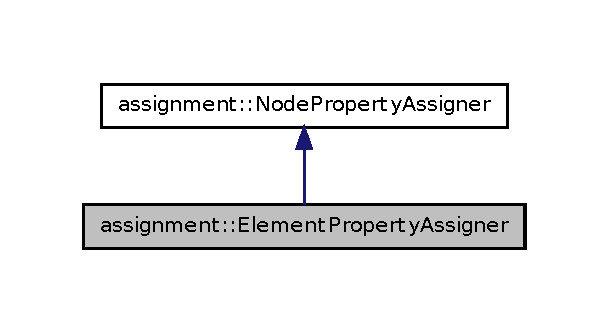
\includegraphics[width=292pt]{classassignment_1_1_element_property_assigner__inherit__graph}
\end{center}
\end{figure}


Collaboration diagram for assignment::ElementPropertyAssigner:\nopagebreak
\begin{figure}[H]
\begin{center}
\leavevmode
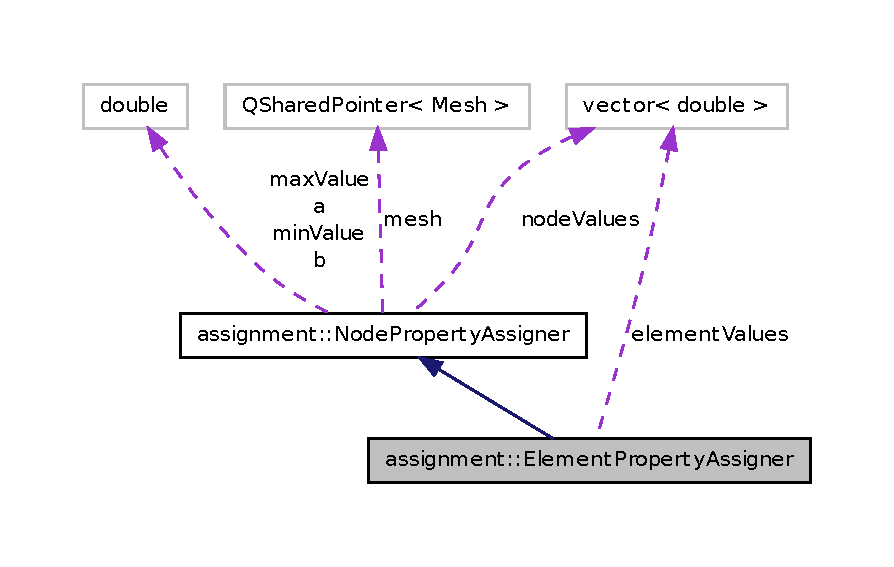
\includegraphics[width=400pt]{classassignment_1_1_element_property_assigner__coll__graph}
\end{center}
\end{figure}
\subsection*{Public Member Functions}
\begin{DoxyCompactItemize}
\item 
\hyperlink{classassignment_1_1_element_property_assigner_a6c7993d7aad6990a1aea6f28731d708c}{ElementPropertyAssigner} (QSharedPointer$<$ \hyperlink{classctimage_1_1_c_t_image}{CTImage} $>$, QSharedPointer$<$ \hyperlink{classmesh_1_1_mesh}{Mesh} $>$, int interpolationMethod, double \hyperlink{classassignment_1_1_node_property_assigner_a7bac7369b89b3351b2ff889114daaf6a}{a}, double \hyperlink{classassignment_1_1_node_property_assigner_a8d2dcf867efc99c60f076cc5d1d55114}{b})
\begin{DoxyCompactList}\small\item\em Creates a new assigner. \item\end{DoxyCompactList}\item 
vector$<$ double $>$ $\ast$ \hyperlink{classassignment_1_1_element_property_assigner_a3e555b9c99bef921efd6c91ae5ee4c32}{getElementValues} ()
\begin{DoxyCompactList}\small\item\em Gets the calculated values in ascending element id order. \item\end{DoxyCompactList}\end{DoxyCompactItemize}
\subsection*{Protected Attributes}
\begin{DoxyCompactItemize}
\item 
\hypertarget{classassignment_1_1_element_property_assigner_aabce575fea3bca22d13c31b2e7220860}{
vector$<$ double $>$ \hyperlink{classassignment_1_1_element_property_assigner_aabce575fea3bca22d13c31b2e7220860}{elementValues}}
\label{classassignment_1_1_element_property_assigner_aabce575fea3bca22d13c31b2e7220860}

\begin{DoxyCompactList}\small\item\em The calculated element values. \item\end{DoxyCompactList}\end{DoxyCompactItemize}


\subsection{Detailed Description}
Assigns CT image data to the elements of a \hyperlink{classmesh_1_1_mesh}{mesh::Mesh}. 

\subsection{Constructor \& Destructor Documentation}
\hypertarget{classassignment_1_1_element_property_assigner_a6c7993d7aad6990a1aea6f28731d708c}{
\index{assignment::ElementPropertyAssigner@{assignment::ElementPropertyAssigner}!ElementPropertyAssigner@{ElementPropertyAssigner}}
\index{ElementPropertyAssigner@{ElementPropertyAssigner}!assignment::ElementPropertyAssigner@{assignment::ElementPropertyAssigner}}
\subsubsection[{ElementPropertyAssigner}]{\setlength{\rightskip}{0pt plus 5cm}assignment::ElementPropertyAssigner::ElementPropertyAssigner (
\begin{DoxyParamCaption}
\item[{QSharedPointer$<$ {\bf CTImage} $>$}]{ ctImage, }
\item[{QSharedPointer$<$ {\bf Mesh} $>$}]{ mesh, }
\item[{int}]{ interpolationMethod, }
\item[{double}]{ a, }
\item[{double}]{ b}
\end{DoxyParamCaption}
)}}
\label{classassignment_1_1_element_property_assigner_a6c7993d7aad6990a1aea6f28731d708c}


Creates a new assigner. 


\begin{DoxyParams}{Parameters}
\item[{\em ctimage}]The \hyperlink{classctimage_1_1_c_t_image}{ctimage::CTImage} \item[{\em mesh}]The \hyperlink{classmesh_1_1_mesh}{mesh::Mesh} \item[{\em interpolationMethod}]The interpolation method \item[{\em a}]The first parameter for the assignment law \item[{\em b}]The second parameter for the assignment law \end{DoxyParams}


\subsection{Member Function Documentation}
\hypertarget{classassignment_1_1_element_property_assigner_a3e555b9c99bef921efd6c91ae5ee4c32}{
\index{assignment::ElementPropertyAssigner@{assignment::ElementPropertyAssigner}!getElementValues@{getElementValues}}
\index{getElementValues@{getElementValues}!assignment::ElementPropertyAssigner@{assignment::ElementPropertyAssigner}}
\subsubsection[{getElementValues}]{\setlength{\rightskip}{0pt plus 5cm}vector$<$ double $>$ $\ast$ assignment::ElementPropertyAssigner::getElementValues (
\begin{DoxyParamCaption}
{}
\end{DoxyParamCaption}
)}}
\label{classassignment_1_1_element_property_assigner_a3e555b9c99bef921efd6c91ae5ee4c32}


Gets the calculated values in ascending element id order. 

\begin{DoxyReturn}{Returns}
The vector containing the element values 
\end{DoxyReturn}


The documentation for this class was generated from the following files:\begin{DoxyCompactItemize}
\item 
assignment/ElementPropertyAssigner.h\item 
assignment/ElementPropertyAssigner.cxx\end{DoxyCompactItemize}

\hypertarget{classassignment_1_1_interpolator3_d}{
\section{assignment::Interpolator3D Class Reference}
\label{classassignment_1_1_interpolator3_d}\index{assignment::Interpolator3D@{assignment::Interpolator3D}}
}


Interpolates a \hyperlink{structmesh_1_1_mesh_1_1_point}{mesh::Mesh::Point} inside a CTImage.  




{\ttfamily \#include $<$Interpolator3D.h$>$}



Inheritance diagram for assignment::Interpolator3D:\nopagebreak
\begin{figure}[H]
\begin{center}
\leavevmode
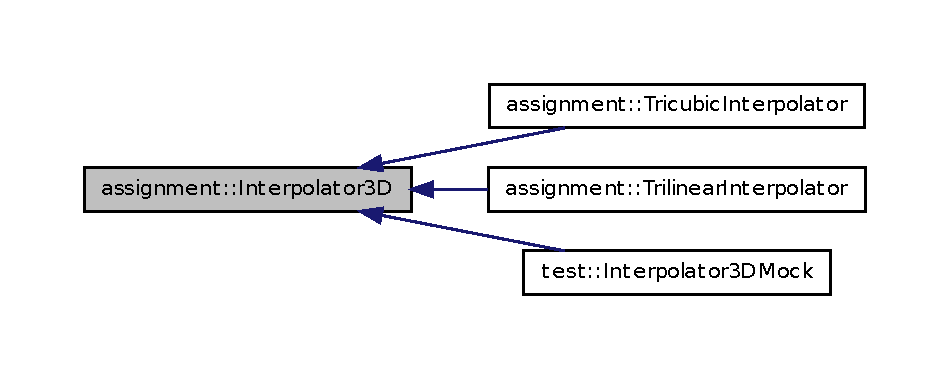
\includegraphics[width=400pt]{classassignment_1_1_interpolator3_d__inherit__graph}
\end{center}
\end{figure}


Collaboration diagram for assignment::Interpolator3D:\nopagebreak
\begin{figure}[H]
\begin{center}
\leavevmode
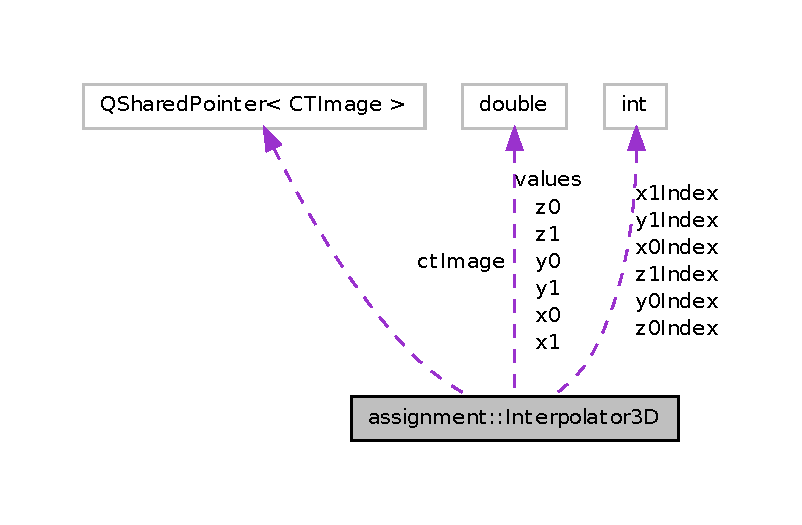
\includegraphics[width=385pt]{classassignment_1_1_interpolator3_d__coll__graph}
\end{center}
\end{figure}
\subsection*{Public Member Functions}
\begin{DoxyCompactItemize}
\item 
\hyperlink{classassignment_1_1_interpolator3_d_a54645d60de51db0881e97c085e0a4c75}{Interpolator3D} (QSharedPointer$<$ \hyperlink{classctimage_1_1_c_t_image}{CTImage} $>$ \hyperlink{classassignment_1_1_interpolator3_d_a7a9b457f60bd12527e0402fcab391bf3}{ctImage}, double $\ast$\hyperlink{classassignment_1_1_interpolator3_d_a061525dc9657ecd0aac93d647398e01f}{values})
\begin{DoxyCompactList}\small\item\em Creates a new interpolator with a given \hyperlink{classctimage_1_1_c_t_image}{ctimage::CTImage} and the values used for the interpolation. \item\end{DoxyCompactList}\item 
virtual double \hyperlink{classassignment_1_1_interpolator3_d_ac6ed5447418b7980d5ad2f12e853b35f}{getValue} (\hyperlink{structmesh_1_1_mesh_1_1_point}{Mesh::Point} $\ast$p)=0
\begin{DoxyCompactList}\small\item\em Gets the interpolated value for a specified \hyperlink{structmesh_1_1_mesh_1_1_point}{mesh::Mesh::Point}. \item\end{DoxyCompactList}\end{DoxyCompactItemize}
\subsection*{Protected Member Functions}
\begin{DoxyCompactItemize}
\item 
int \hyperlink{classassignment_1_1_interpolator3_d_a2fd5d0ea20ee345a485d6b6aba546bf7}{getIndex} (int x, int y, int z)
\begin{DoxyCompactList}\small\item\em Gets the index for the values array, given xyz coordinate indexes. \item\end{DoxyCompactList}\item 
void \hyperlink{classassignment_1_1_interpolator3_d_a7f1152d0026def40f616d2c8c33844fd}{setUpCube} (\hyperlink{structmesh_1_1_mesh_1_1_point}{Mesh::Point} $\ast$p)
\begin{DoxyCompactList}\small\item\em Sets the members for the cube surrounding the current interpolation point. \item\end{DoxyCompactList}\end{DoxyCompactItemize}
\subsection*{Protected Attributes}
\begin{DoxyCompactItemize}
\item 
\hypertarget{classassignment_1_1_interpolator3_d_a7a9b457f60bd12527e0402fcab391bf3}{
QSharedPointer$<$ \hyperlink{classctimage_1_1_c_t_image}{CTImage} $>$ \hyperlink{classassignment_1_1_interpolator3_d_a7a9b457f60bd12527e0402fcab391bf3}{ctImage}}
\label{classassignment_1_1_interpolator3_d_a7a9b457f60bd12527e0402fcab391bf3}

\begin{DoxyCompactList}\small\item\em A pointer to the \hyperlink{classctimage_1_1_c_t_image}{ctimage::CTImage}. \item\end{DoxyCompactList}\item 
\hypertarget{classassignment_1_1_interpolator3_d_a061525dc9657ecd0aac93d647398e01f}{
double $\ast$ \hyperlink{classassignment_1_1_interpolator3_d_a061525dc9657ecd0aac93d647398e01f}{values}}
\label{classassignment_1_1_interpolator3_d_a061525dc9657ecd0aac93d647398e01f}

\begin{DoxyCompactList}\small\item\em The values to be used for the interpolation. \item\end{DoxyCompactList}\item 
\hypertarget{classassignment_1_1_interpolator3_d_afb656ddf8789b483a8570f7a93985c0c}{
double \hyperlink{classassignment_1_1_interpolator3_d_afb656ddf8789b483a8570f7a93985c0c}{x0}}
\label{classassignment_1_1_interpolator3_d_afb656ddf8789b483a8570f7a93985c0c}

\begin{DoxyCompactList}\small\item\em The first edge x-\/coordinate of the cube surrounding the current interpolation point. \item\end{DoxyCompactList}\item 
\hypertarget{classassignment_1_1_interpolator3_d_ab8f3111100189b5730621f77fe54467e}{
double \hyperlink{classassignment_1_1_interpolator3_d_ab8f3111100189b5730621f77fe54467e}{x1}}
\label{classassignment_1_1_interpolator3_d_ab8f3111100189b5730621f77fe54467e}

\begin{DoxyCompactList}\small\item\em The second x-\/coordinate of the cube surrounding the current interpolation point. \item\end{DoxyCompactList}\item 
\hypertarget{classassignment_1_1_interpolator3_d_a42b29917bd0265791560f4ddc697f7ea}{
double \hyperlink{classassignment_1_1_interpolator3_d_a42b29917bd0265791560f4ddc697f7ea}{y0}}
\label{classassignment_1_1_interpolator3_d_a42b29917bd0265791560f4ddc697f7ea}

\begin{DoxyCompactList}\small\item\em The first edge y-\/coordinate of the cube surrounding the current interpolation point. \item\end{DoxyCompactList}\item 
\hypertarget{classassignment_1_1_interpolator3_d_ad5cd282be05bb14625807880ed3fc322}{
double \hyperlink{classassignment_1_1_interpolator3_d_ad5cd282be05bb14625807880ed3fc322}{y1}}
\label{classassignment_1_1_interpolator3_d_ad5cd282be05bb14625807880ed3fc322}

\begin{DoxyCompactList}\small\item\em The second edge y-\/coordinate of the cube surrounding the current interpolation point. \item\end{DoxyCompactList}\item 
\hypertarget{classassignment_1_1_interpolator3_d_a9a1fcc6b430714b7171ff2e41a8ced79}{
double \hyperlink{classassignment_1_1_interpolator3_d_a9a1fcc6b430714b7171ff2e41a8ced79}{z0}}
\label{classassignment_1_1_interpolator3_d_a9a1fcc6b430714b7171ff2e41a8ced79}

\begin{DoxyCompactList}\small\item\em The first edge z-\/coordinate of the cube surrounding the current interpolation point. \item\end{DoxyCompactList}\item 
\hypertarget{classassignment_1_1_interpolator3_d_a98c11cc781d0338f6049e186011988b3}{
double \hyperlink{classassignment_1_1_interpolator3_d_a98c11cc781d0338f6049e186011988b3}{z1}}
\label{classassignment_1_1_interpolator3_d_a98c11cc781d0338f6049e186011988b3}

\begin{DoxyCompactList}\small\item\em The second edge z-\/coordinate of the cube surrounding the current interpolation point. \item\end{DoxyCompactList}\item 
\hypertarget{classassignment_1_1_interpolator3_d_a5f5958cc28894f071c910f3a6950b4a7}{
int \hyperlink{classassignment_1_1_interpolator3_d_a5f5958cc28894f071c910f3a6950b4a7}{x0Index}}
\label{classassignment_1_1_interpolator3_d_a5f5958cc28894f071c910f3a6950b4a7}

\begin{DoxyCompactList}\small\item\em The first x-\/coordinate edge index value of the cube surrounding the current interpolation point. \item\end{DoxyCompactList}\item 
\hypertarget{classassignment_1_1_interpolator3_d_ae1801f9719cc067f46cc4dbad850584e}{
int \hyperlink{classassignment_1_1_interpolator3_d_ae1801f9719cc067f46cc4dbad850584e}{x1Index}}
\label{classassignment_1_1_interpolator3_d_ae1801f9719cc067f46cc4dbad850584e}

\begin{DoxyCompactList}\small\item\em The second x-\/coordinate edge index value of the cube surrounding the current interpolation point. \item\end{DoxyCompactList}\item 
\hypertarget{classassignment_1_1_interpolator3_d_a510c7513371c0a901b5d382dda2eb522}{
int \hyperlink{classassignment_1_1_interpolator3_d_a510c7513371c0a901b5d382dda2eb522}{y0Index}}
\label{classassignment_1_1_interpolator3_d_a510c7513371c0a901b5d382dda2eb522}

\begin{DoxyCompactList}\small\item\em The first y-\/coordinate edge index value of the cube surrounding the current interpolation point. \item\end{DoxyCompactList}\item 
\hypertarget{classassignment_1_1_interpolator3_d_a7915e8474ca9f2d24a6db89a4e6392aa}{
int \hyperlink{classassignment_1_1_interpolator3_d_a7915e8474ca9f2d24a6db89a4e6392aa}{y1Index}}
\label{classassignment_1_1_interpolator3_d_a7915e8474ca9f2d24a6db89a4e6392aa}

\begin{DoxyCompactList}\small\item\em The second y-\/coordinate edge index value of the cube surrounding the current interpolation point. \item\end{DoxyCompactList}\item 
\hypertarget{classassignment_1_1_interpolator3_d_a35aef5fb165edabee98473cce828f26a}{
int \hyperlink{classassignment_1_1_interpolator3_d_a35aef5fb165edabee98473cce828f26a}{z0Index}}
\label{classassignment_1_1_interpolator3_d_a35aef5fb165edabee98473cce828f26a}

\begin{DoxyCompactList}\small\item\em The first z-\/coordinate edge index value of the cube surrounding the current interpolation point. \item\end{DoxyCompactList}\item 
\hypertarget{classassignment_1_1_interpolator3_d_a5160d595a9c9884e38b7d8e64d01f9b8}{
int \hyperlink{classassignment_1_1_interpolator3_d_a5160d595a9c9884e38b7d8e64d01f9b8}{z1Index}}
\label{classassignment_1_1_interpolator3_d_a5160d595a9c9884e38b7d8e64d01f9b8}

\begin{DoxyCompactList}\small\item\em The second z-\/coordinate edge index value of the cube surrounding the current interpolation point. \item\end{DoxyCompactList}\end{DoxyCompactItemize}


\subsection{Detailed Description}
Interpolates a \hyperlink{structmesh_1_1_mesh_1_1_point}{mesh::Mesh::Point} inside a CTImage. 

\subsection{Constructor \& Destructor Documentation}
\hypertarget{classassignment_1_1_interpolator3_d_a54645d60de51db0881e97c085e0a4c75}{
\index{assignment::Interpolator3D@{assignment::Interpolator3D}!Interpolator3D@{Interpolator3D}}
\index{Interpolator3D@{Interpolator3D}!assignment::Interpolator3D@{assignment::Interpolator3D}}
\subsubsection[{Interpolator3D}]{\setlength{\rightskip}{0pt plus 5cm}assignment::Interpolator3D::Interpolator3D (
\begin{DoxyParamCaption}
\item[{QSharedPointer$<$ {\bf CTImage} $>$}]{ ctImage, }
\item[{double $\ast$}]{ values}
\end{DoxyParamCaption}
)}}
\label{classassignment_1_1_interpolator3_d_a54645d60de51db0881e97c085e0a4c75}


Creates a new interpolator with a given \hyperlink{classctimage_1_1_c_t_image}{ctimage::CTImage} and the values used for the interpolation. 


\begin{DoxyParams}{Parameters}
\item[{\em ctImage}]The \hyperlink{classctimage_1_1_c_t_image}{ctimage::CTImage}, which is used only for morphologic information. The values of the \hyperlink{classctimage_1_1_c_t_image}{ctimage::CTImage} are not used for the interpolation \item[{\em values}]The values used for the interpolation. The values array needs to be the size of the pixel count of the \hyperlink{classctimage_1_1_c_t_image}{ctimage::CTImage} \end{DoxyParams}


\subsection{Member Function Documentation}
\hypertarget{classassignment_1_1_interpolator3_d_a2fd5d0ea20ee345a485d6b6aba546bf7}{
\index{assignment::Interpolator3D@{assignment::Interpolator3D}!getIndex@{getIndex}}
\index{getIndex@{getIndex}!assignment::Interpolator3D@{assignment::Interpolator3D}}
\subsubsection[{getIndex}]{\setlength{\rightskip}{0pt plus 5cm}int assignment::Interpolator3D::getIndex (
\begin{DoxyParamCaption}
\item[{int}]{ x, }
\item[{int}]{ y, }
\item[{int}]{ z}
\end{DoxyParamCaption}
)\hspace{0.3cm}{\ttfamily  \mbox{[}protected\mbox{]}}}}
\label{classassignment_1_1_interpolator3_d_a2fd5d0ea20ee345a485d6b6aba546bf7}


Gets the index for the values array, given xyz coordinate indexes. 


\begin{DoxyParams}{Parameters}
\item[{\em x}]x index \item[{\em y}]y index \item[{\em z}]z index \end{DoxyParams}
\begin{DoxyReturn}{Returns}
The index value 
\end{DoxyReturn}
\hypertarget{classassignment_1_1_interpolator3_d_ac6ed5447418b7980d5ad2f12e853b35f}{
\index{assignment::Interpolator3D@{assignment::Interpolator3D}!getValue@{getValue}}
\index{getValue@{getValue}!assignment::Interpolator3D@{assignment::Interpolator3D}}
\subsubsection[{getValue}]{\setlength{\rightskip}{0pt plus 5cm}virtual double assignment::Interpolator3D::getValue (
\begin{DoxyParamCaption}
\item[{{\bf Mesh::Point} $\ast$}]{ p}
\end{DoxyParamCaption}
)\hspace{0.3cm}{\ttfamily  \mbox{[}pure virtual\mbox{]}}}}
\label{classassignment_1_1_interpolator3_d_ac6ed5447418b7980d5ad2f12e853b35f}


Gets the interpolated value for a specified \hyperlink{structmesh_1_1_mesh_1_1_point}{mesh::Mesh::Point}. 


\begin{DoxyParams}{Parameters}
\item[{\em p}]The point to be interpolated \end{DoxyParams}


Implemented in \hyperlink{classassignment_1_1_tricubic_interpolator_ac06870dcde750c17f2d7ce02b87cbd9c}{assignment::TricubicInterpolator}, \hyperlink{classassignment_1_1_trilinear_interpolator_a0972e2f1ebd828b832e94760c34b80c6}{assignment::TrilinearInterpolator}, and \hyperlink{classtest_1_1_interpolator3_d_mock_aff76393fb25a4a23db2039b074af75b2}{test::Interpolator3DMock}.

\hypertarget{classassignment_1_1_interpolator3_d_a7f1152d0026def40f616d2c8c33844fd}{
\index{assignment::Interpolator3D@{assignment::Interpolator3D}!setUpCube@{setUpCube}}
\index{setUpCube@{setUpCube}!assignment::Interpolator3D@{assignment::Interpolator3D}}
\subsubsection[{setUpCube}]{\setlength{\rightskip}{0pt plus 5cm}void assignment::Interpolator3D::setUpCube (
\begin{DoxyParamCaption}
\item[{{\bf Mesh::Point} $\ast$}]{ p}
\end{DoxyParamCaption}
)\hspace{0.3cm}{\ttfamily  \mbox{[}protected\mbox{]}}}}
\label{classassignment_1_1_interpolator3_d_a7f1152d0026def40f616d2c8c33844fd}


Sets the members for the cube surrounding the current interpolation point. 


\begin{DoxyParams}{Parameters}
\item[{\em p}]The point to be interpolated \end{DoxyParams}


The documentation for this class was generated from the following files:\begin{DoxyCompactItemize}
\item 
assignment/Interpolator3D.h\item 
assignment/Interpolator3D.cxx\end{DoxyCompactItemize}

\hypertarget{classassignment_1_1_node_property_assigner}{
\section{assignment::NodePropertyAssigner Class Reference}
\label{classassignment_1_1_node_property_assigner}\index{assignment::NodePropertyAssigner@{assignment::NodePropertyAssigner}}
}


Assigns CT image data to the nodes of a \hyperlink{classmesh_1_1_mesh}{mesh::Mesh}.  




{\ttfamily \#include $<$NodePropertyAssigner.h$>$}



Inheritance diagram for assignment::NodePropertyAssigner:\nopagebreak
\begin{figure}[H]
\begin{center}
\leavevmode
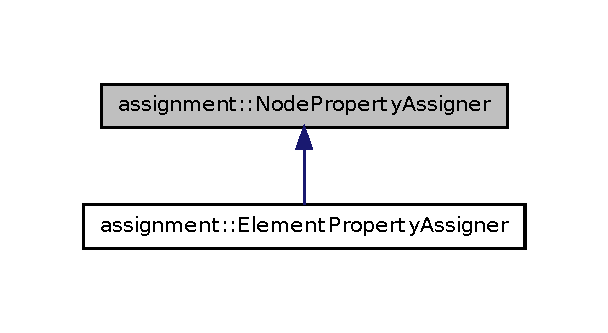
\includegraphics[width=292pt]{classassignment_1_1_node_property_assigner__inherit__graph}
\end{center}
\end{figure}


Collaboration diagram for assignment::NodePropertyAssigner:\nopagebreak
\begin{figure}[H]
\begin{center}
\leavevmode
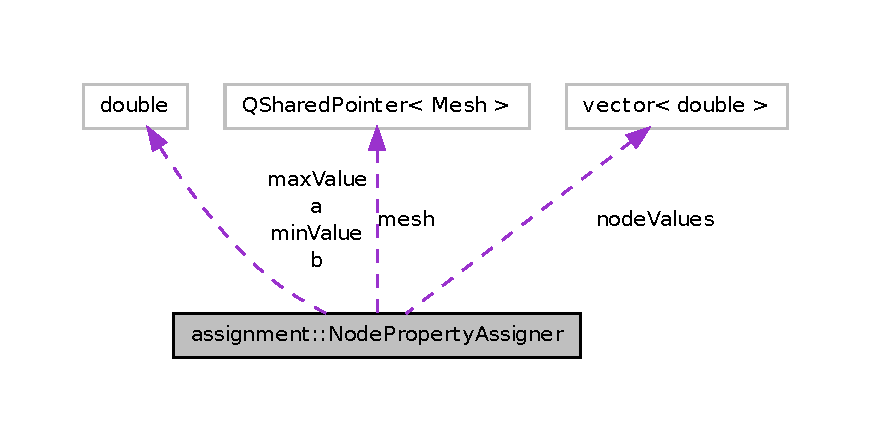
\includegraphics[width=400pt]{classassignment_1_1_node_property_assigner__coll__graph}
\end{center}
\end{figure}
\subsection*{Public Member Functions}
\begin{DoxyCompactItemize}
\item 
\hyperlink{classassignment_1_1_node_property_assigner_afc4761487858cccc6a66dfa949984e3a}{NodePropertyAssigner} (QSharedPointer$<$ \hyperlink{classctimage_1_1_c_t_image}{CTImage} $>$ ctimage, QSharedPointer$<$ \hyperlink{classmesh_1_1_mesh}{Mesh} $>$ \hyperlink{classassignment_1_1_node_property_assigner_a91e04d259955ce0ae93d02760ac2945e}{mesh}, int interpolationMethod, double \hyperlink{classassignment_1_1_node_property_assigner_a7bac7369b89b3351b2ff889114daaf6a}{a}, double \hyperlink{classassignment_1_1_node_property_assigner_a8d2dcf867efc99c60f076cc5d1d55114}{b})
\begin{DoxyCompactList}\small\item\em Creates a new assigner. \item\end{DoxyCompactList}\item 
\hypertarget{classassignment_1_1_node_property_assigner_a9c023c3f2d6dd830f6c64958650bf177}{
QSharedPointer$<$ \hyperlink{classmesh_1_1_mesh}{Mesh} $>$ \hyperlink{classassignment_1_1_node_property_assigner_a9c023c3f2d6dd830f6c64958650bf177}{getMesh} ()}
\label{classassignment_1_1_node_property_assigner_a9c023c3f2d6dd830f6c64958650bf177}

\begin{DoxyCompactList}\small\item\em Gets the \hyperlink{classmesh_1_1_mesh}{mesh::Mesh} that is used for the assignment. \item\end{DoxyCompactList}\item 
\hypertarget{classassignment_1_1_node_property_assigner_ae157e095fda36f722c9ddb3d2a2492af}{
double \hyperlink{classassignment_1_1_node_property_assigner_ae157e095fda36f722c9ddb3d2a2492af}{getMinValue} ()}
\label{classassignment_1_1_node_property_assigner_ae157e095fda36f722c9ddb3d2a2492af}

\begin{DoxyCompactList}\small\item\em Gets the minimum value of the assignment. \item\end{DoxyCompactList}\item 
\hypertarget{classassignment_1_1_node_property_assigner_a9ff48294b2759b8c46d2673cd3f87731}{
double \hyperlink{classassignment_1_1_node_property_assigner_a9ff48294b2759b8c46d2673cd3f87731}{getMaxValue} ()}
\label{classassignment_1_1_node_property_assigner_a9ff48294b2759b8c46d2673cd3f87731}

\begin{DoxyCompactList}\small\item\em Gets the maximum value of the assignment. \item\end{DoxyCompactList}\item 
\hypertarget{classassignment_1_1_node_property_assigner_afc2fb3b88d92a968c65b5759a9fe1411}{
vector$<$ double $>$ $\ast$ \hyperlink{classassignment_1_1_node_property_assigner_afc2fb3b88d92a968c65b5759a9fe1411}{getNodeValues} ()}
\label{classassignment_1_1_node_property_assigner_afc2fb3b88d92a968c65b5759a9fe1411}

\begin{DoxyCompactList}\small\item\em Gets the assigned node values. \item\end{DoxyCompactList}\end{DoxyCompactItemize}
\subsection*{Protected Member Functions}
\begin{DoxyCompactItemize}
\item 
double $\ast$ \hyperlink{classassignment_1_1_node_property_assigner_af6a16969141073a2af5b898a3b69cf55}{ashDensityRev} (int n, \hyperlink{classctimage_1_1_c_t_image_ab3bf32a276d168a705973d8d6c698cec}{CTImage::CTPixelType} $\ast$ct)
\begin{DoxyCompactList}\small\item\em Returns the calculated density of a CT image's pixels. \item\end{DoxyCompactList}\end{DoxyCompactItemize}
\subsection*{Protected Attributes}
\begin{DoxyCompactItemize}
\item 
\hypertarget{classassignment_1_1_node_property_assigner_a91e04d259955ce0ae93d02760ac2945e}{
QSharedPointer$<$ \hyperlink{classmesh_1_1_mesh}{Mesh} $>$ \hyperlink{classassignment_1_1_node_property_assigner_a91e04d259955ce0ae93d02760ac2945e}{mesh}}
\label{classassignment_1_1_node_property_assigner_a91e04d259955ce0ae93d02760ac2945e}

\begin{DoxyCompactList}\small\item\em The \hyperlink{classmesh_1_1_mesh}{mesh::Mesh} the values are assigned to. \item\end{DoxyCompactList}\item 
\hypertarget{classassignment_1_1_node_property_assigner_ab16e117511d9e34142a7052f665ea118}{
vector$<$ double $>$ \hyperlink{classassignment_1_1_node_property_assigner_ab16e117511d9e34142a7052f665ea118}{nodeValues}}
\label{classassignment_1_1_node_property_assigner_ab16e117511d9e34142a7052f665ea118}

\begin{DoxyCompactList}\small\item\em A vector containing the assigned node values. \item\end{DoxyCompactList}\item 
\hypertarget{classassignment_1_1_node_property_assigner_a56ca01884fce9dde775e3d5f83ef553b}{
double \hyperlink{classassignment_1_1_node_property_assigner_a56ca01884fce9dde775e3d5f83ef553b}{minValue}}
\label{classassignment_1_1_node_property_assigner_a56ca01884fce9dde775e3d5f83ef553b}

\begin{DoxyCompactList}\small\item\em The minimum value of the assignment. \item\end{DoxyCompactList}\item 
\hypertarget{classassignment_1_1_node_property_assigner_a117253a9d4f13c778dda1d6fbf09b885}{
double \hyperlink{classassignment_1_1_node_property_assigner_a117253a9d4f13c778dda1d6fbf09b885}{maxValue}}
\label{classassignment_1_1_node_property_assigner_a117253a9d4f13c778dda1d6fbf09b885}

\begin{DoxyCompactList}\small\item\em The maximum value of the assignment. \item\end{DoxyCompactList}\item 
\hypertarget{classassignment_1_1_node_property_assigner_a7bac7369b89b3351b2ff889114daaf6a}{
double \hyperlink{classassignment_1_1_node_property_assigner_a7bac7369b89b3351b2ff889114daaf6a}{a}}
\label{classassignment_1_1_node_property_assigner_a7bac7369b89b3351b2ff889114daaf6a}

\begin{DoxyCompactList}\small\item\em The first parameter for the assignment law. \item\end{DoxyCompactList}\item 
\hypertarget{classassignment_1_1_node_property_assigner_a8d2dcf867efc99c60f076cc5d1d55114}{
double \hyperlink{classassignment_1_1_node_property_assigner_a8d2dcf867efc99c60f076cc5d1d55114}{b}}
\label{classassignment_1_1_node_property_assigner_a8d2dcf867efc99c60f076cc5d1d55114}

\begin{DoxyCompactList}\small\item\em The second parameter for the assignment law. \item\end{DoxyCompactList}\end{DoxyCompactItemize}


\subsection{Detailed Description}
Assigns CT image data to the nodes of a \hyperlink{classmesh_1_1_mesh}{mesh::Mesh}. 

\subsection{Constructor \& Destructor Documentation}
\hypertarget{classassignment_1_1_node_property_assigner_afc4761487858cccc6a66dfa949984e3a}{
\index{assignment::NodePropertyAssigner@{assignment::NodePropertyAssigner}!NodePropertyAssigner@{NodePropertyAssigner}}
\index{NodePropertyAssigner@{NodePropertyAssigner}!assignment::NodePropertyAssigner@{assignment::NodePropertyAssigner}}
\subsubsection[{NodePropertyAssigner}]{\setlength{\rightskip}{0pt plus 5cm}assignment::NodePropertyAssigner::NodePropertyAssigner (
\begin{DoxyParamCaption}
\item[{QSharedPointer$<$ {\bf CTImage} $>$}]{ ctimage, }
\item[{QSharedPointer$<$ {\bf Mesh} $>$}]{ mesh, }
\item[{int}]{ interpolationMethod, }
\item[{double}]{ a, }
\item[{double}]{ b}
\end{DoxyParamCaption}
)}}
\label{classassignment_1_1_node_property_assigner_afc4761487858cccc6a66dfa949984e3a}


Creates a new assigner. 


\begin{DoxyParams}{Parameters}
\item[{\em ctimage}]The \hyperlink{classctimage_1_1_c_t_image}{ctimage::CTImage} \item[{\em mesh}]The \hyperlink{classmesh_1_1_mesh}{mesh::Mesh} \item[{\em interpolationMethod}]The interpolation method \item[{\em a}]The first parameter for the assignment law \item[{\em b}]The second parameter for the assignment law \end{DoxyParams}


\subsection{Member Function Documentation}
\hypertarget{classassignment_1_1_node_property_assigner_af6a16969141073a2af5b898a3b69cf55}{
\index{assignment::NodePropertyAssigner@{assignment::NodePropertyAssigner}!ashDensityRev@{ashDensityRev}}
\index{ashDensityRev@{ashDensityRev}!assignment::NodePropertyAssigner@{assignment::NodePropertyAssigner}}
\subsubsection[{ashDensityRev}]{\setlength{\rightskip}{0pt plus 5cm}double $\ast$ assignment::NodePropertyAssigner::ashDensityRev (
\begin{DoxyParamCaption}
\item[{int}]{ n, }
\item[{{\bf CTImage::CTPixelType} $\ast$}]{ ct}
\end{DoxyParamCaption}
)\hspace{0.3cm}{\ttfamily  \mbox{[}protected\mbox{]}}}}
\label{classassignment_1_1_node_property_assigner_af6a16969141073a2af5b898a3b69cf55}


Returns the calculated density of a CT image's pixels. 


\begin{DoxyParams}{Parameters}
\item[{\em n}]The total pixel count \item[{\em ct}]The CT image's pixels \end{DoxyParams}
\begin{DoxyReturn}{Returns}
The calculated density values 
\end{DoxyReturn}


The documentation for this class was generated from the following files:\begin{DoxyCompactItemize}
\item 
assignment/NodePropertyAssigner.h\item 
assignment/NodePropertyAssigner.cxx\end{DoxyCompactItemize}

\hypertarget{classassignment_1_1_tricubic_interpolator}{
\section{assignment::TricubicInterpolator Class Reference}
\label{classassignment_1_1_tricubic_interpolator}\index{assignment::TricubicInterpolator@{assignment::TricubicInterpolator}}
}


Interpolates a \hyperlink{structmesh_1_1_mesh_1_1_point}{mesh::Mesh::Point} tricubic.  




{\ttfamily \#include $<$TricubicInterpolator.h$>$}



Inheritance diagram for assignment::TricubicInterpolator:\nopagebreak
\begin{figure}[H]
\begin{center}
\leavevmode
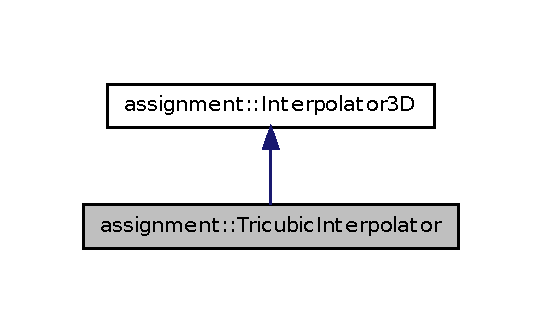
\includegraphics[width=260pt]{classassignment_1_1_tricubic_interpolator__inherit__graph}
\end{center}
\end{figure}


Collaboration diagram for assignment::TricubicInterpolator:\nopagebreak
\begin{figure}[H]
\begin{center}
\leavevmode
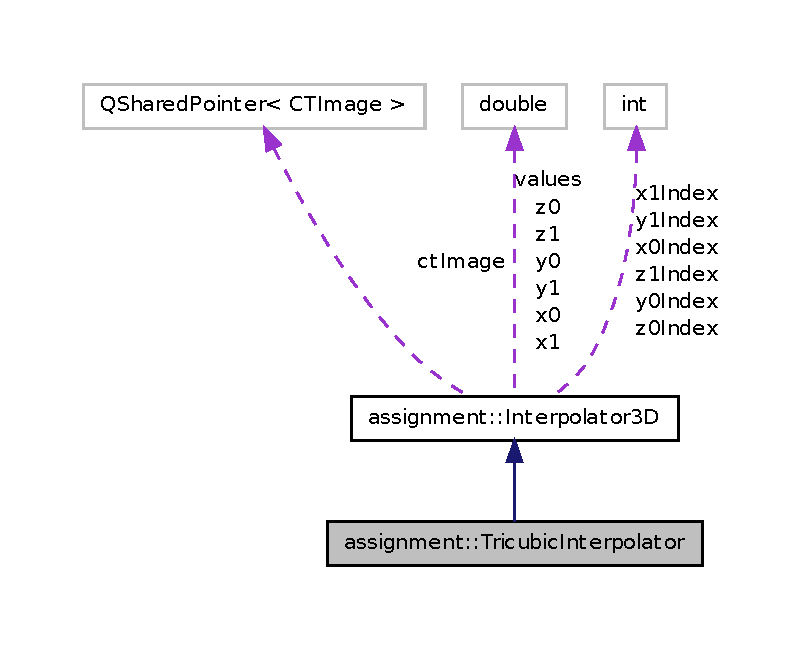
\includegraphics[width=385pt]{classassignment_1_1_tricubic_interpolator__coll__graph}
\end{center}
\end{figure}
\subsection*{Classes}
\begin{DoxyCompactItemize}
\item 
struct \hyperlink{structassignment_1_1_tricubic_interpolator_1_1_sample}{Sample}
\end{DoxyCompactItemize}
\subsection*{Public Member Functions}
\begin{DoxyCompactItemize}
\item 
\hyperlink{classassignment_1_1_tricubic_interpolator_ac582527ae93e8532fafb7bbc75a14f6c}{TricubicInterpolator} (QSharedPointer$<$ \hyperlink{classctimage_1_1_c_t_image}{CTImage} $>$, double $\ast$)
\begin{DoxyCompactList}\small\item\em Creates a new tricubic interpolator with a given \hyperlink{classctimage_1_1_c_t_image}{ctimage::CTImage} and the values used for the interpolation. \item\end{DoxyCompactList}\item 
double \hyperlink{classassignment_1_1_tricubic_interpolator_ac06870dcde750c17f2d7ce02b87cbd9c}{getValue} (\hyperlink{structmesh_1_1_mesh_1_1_point}{Mesh::Point} $\ast$)
\begin{DoxyCompactList}\small\item\em Gets the interpolated value for a specified \hyperlink{structmesh_1_1_mesh_1_1_point}{mesh::Mesh::Point}. \item\end{DoxyCompactList}\end{DoxyCompactItemize}
\subsection*{Private Member Functions}
\begin{DoxyCompactItemize}
\item 
double \hyperlink{classassignment_1_1_tricubic_interpolator_afcf8e9955ee7e7852e60ebd4e1187750}{interpolateCubic} (\hyperlink{structassignment_1_1_tricubic_interpolator_1_1_sample}{Sample} $\ast$sample, double x)
\begin{DoxyCompactList}\small\item\em Returns the result of cubic interpolation between 4 \hyperlink{structassignment_1_1_tricubic_interpolator_1_1_sample}{Sample} points. \item\end{DoxyCompactList}\item 
double \hyperlink{classassignment_1_1_tricubic_interpolator_a58acbe3aef7780ce192dca441a39be1c}{interpolateBicubic} (int zIndex, double x, double y)
\begin{DoxyCompactList}\small\item\em Returns the result of bicubic interpolation inside a z-\/slice of the 4x4x4 grid surrounding the point to be interpolated. \item\end{DoxyCompactList}\end{DoxyCompactItemize}
\subsection*{Friends}
\begin{DoxyCompactItemize}
\item 
\hypertarget{classassignment_1_1_tricubic_interpolator_a507b8c8173a81dd673312db5aa36c817}{
class \hyperlink{classassignment_1_1_tricubic_interpolator_a507b8c8173a81dd673312db5aa36c817}{test::TricubicInterpolatorTest}}
\label{classassignment_1_1_tricubic_interpolator_a507b8c8173a81dd673312db5aa36c817}

\end{DoxyCompactItemize}


\subsection{Detailed Description}
Interpolates a \hyperlink{structmesh_1_1_mesh_1_1_point}{mesh::Mesh::Point} tricubic. \begin{DoxyNote}{Note}
\href{http://en.wikipedia.org/wiki/Tricubic_interpolation}{\tt http://en.wikipedia.org/wiki/Tricubic\_\-interpolation} 
\end{DoxyNote}


\subsection{Constructor \& Destructor Documentation}
\hypertarget{classassignment_1_1_tricubic_interpolator_ac582527ae93e8532fafb7bbc75a14f6c}{
\index{assignment::TricubicInterpolator@{assignment::TricubicInterpolator}!TricubicInterpolator@{TricubicInterpolator}}
\index{TricubicInterpolator@{TricubicInterpolator}!assignment::TricubicInterpolator@{assignment::TricubicInterpolator}}
\subsubsection[{TricubicInterpolator}]{\setlength{\rightskip}{0pt plus 5cm}assignment::TricubicInterpolator::TricubicInterpolator (
\begin{DoxyParamCaption}
\item[{QSharedPointer$<$ {\bf CTImage} $>$}]{ ctImage, }
\item[{double $\ast$}]{ values}
\end{DoxyParamCaption}
)}}
\label{classassignment_1_1_tricubic_interpolator_ac582527ae93e8532fafb7bbc75a14f6c}


Creates a new tricubic interpolator with a given \hyperlink{classctimage_1_1_c_t_image}{ctimage::CTImage} and the values used for the interpolation. 


\begin{DoxyParams}{Parameters}
\item[{\em ctImage}]The \hyperlink{classctimage_1_1_c_t_image}{ctimage::CTImage}, which is used only for morphologic information. The values of the \hyperlink{classctimage_1_1_c_t_image}{ctimage::CTImage} are not used for the interpolation \item[{\em values}]The values used for the interpolation. The values array needs to be the size of the pixel count of the \hyperlink{classctimage_1_1_c_t_image}{ctimage::CTImage} \end{DoxyParams}


\subsection{Member Function Documentation}
\hypertarget{classassignment_1_1_tricubic_interpolator_ac06870dcde750c17f2d7ce02b87cbd9c}{
\index{assignment::TricubicInterpolator@{assignment::TricubicInterpolator}!getValue@{getValue}}
\index{getValue@{getValue}!assignment::TricubicInterpolator@{assignment::TricubicInterpolator}}
\subsubsection[{getValue}]{\setlength{\rightskip}{0pt plus 5cm}double assignment::TricubicInterpolator::getValue (
\begin{DoxyParamCaption}
\item[{{\bf Mesh::Point} $\ast$}]{ p}
\end{DoxyParamCaption}
)\hspace{0.3cm}{\ttfamily  \mbox{[}virtual\mbox{]}}}}
\label{classassignment_1_1_tricubic_interpolator_ac06870dcde750c17f2d7ce02b87cbd9c}


Gets the interpolated value for a specified \hyperlink{structmesh_1_1_mesh_1_1_point}{mesh::Mesh::Point}. 


\begin{DoxyParams}{Parameters}
\item[{\em p}]The point to be interpolated \end{DoxyParams}


Implements \hyperlink{classassignment_1_1_interpolator3_d_ac6ed5447418b7980d5ad2f12e853b35f}{assignment::Interpolator3D}.

\hypertarget{classassignment_1_1_tricubic_interpolator_a58acbe3aef7780ce192dca441a39be1c}{
\index{assignment::TricubicInterpolator@{assignment::TricubicInterpolator}!interpolateBicubic@{interpolateBicubic}}
\index{interpolateBicubic@{interpolateBicubic}!assignment::TricubicInterpolator@{assignment::TricubicInterpolator}}
\subsubsection[{interpolateBicubic}]{\setlength{\rightskip}{0pt plus 5cm}double assignment::TricubicInterpolator::interpolateBicubic (
\begin{DoxyParamCaption}
\item[{int}]{ zIndex, }
\item[{double}]{ x, }
\item[{double}]{ y}
\end{DoxyParamCaption}
)\hspace{0.3cm}{\ttfamily  \mbox{[}private\mbox{]}}}}
\label{classassignment_1_1_tricubic_interpolator_a58acbe3aef7780ce192dca441a39be1c}


Returns the result of bicubic interpolation inside a z-\/slice of the 4x4x4 grid surrounding the point to be interpolated. 


\begin{DoxyParams}{Parameters}
\item[{\em zIndex}]The z-\/index of the slice \item[{\em x}]The x-\/coordinate of the point to be interpolated \item[{\em y}]The y-\/coordinate of the point to be interpolated \end{DoxyParams}
\begin{DoxyReturn}{Returns}
The interpolation result 
\end{DoxyReturn}
\hypertarget{classassignment_1_1_tricubic_interpolator_afcf8e9955ee7e7852e60ebd4e1187750}{
\index{assignment::TricubicInterpolator@{assignment::TricubicInterpolator}!interpolateCubic@{interpolateCubic}}
\index{interpolateCubic@{interpolateCubic}!assignment::TricubicInterpolator@{assignment::TricubicInterpolator}}
\subsubsection[{interpolateCubic}]{\setlength{\rightskip}{0pt plus 5cm}double assignment::TricubicInterpolator::interpolateCubic (
\begin{DoxyParamCaption}
\item[{{\bf Sample} $\ast$}]{ sample, }
\item[{double}]{ x}
\end{DoxyParamCaption}
)\hspace{0.3cm}{\ttfamily  \mbox{[}private\mbox{]}}}}
\label{classassignment_1_1_tricubic_interpolator_afcf8e9955ee7e7852e60ebd4e1187750}


Returns the result of cubic interpolation between 4 \hyperlink{structassignment_1_1_tricubic_interpolator_1_1_sample}{Sample} points. 

\begin{DoxyWarning}{Warning}
The length of sample must be 4 and the value x must be within the 2nd and the 3rd sample 
\end{DoxyWarning}

\begin{DoxyParams}{Parameters}
\item[{\em sample}]The \hyperlink{structassignment_1_1_tricubic_interpolator_1_1_sample}{Sample} array containing 4 samples \item[{\em x}]The point to be interpolated \end{DoxyParams}
\begin{DoxyReturn}{Returns}
The interpolation result 
\end{DoxyReturn}


The documentation for this class was generated from the following files:\begin{DoxyCompactItemize}
\item 
assignment/TricubicInterpolator.h\item 
assignment/TricubicInterpolator.cxx\end{DoxyCompactItemize}

\hypertarget{structassignment_1_1_tricubic_interpolator_1_1_sample}{
\section{assignment::TricubicInterpolator::Sample Struct Reference}
\label{structassignment_1_1_tricubic_interpolator_1_1_sample}\index{assignment::TricubicInterpolator::Sample@{assignment::TricubicInterpolator::Sample}}
}


Collaboration diagram for assignment::TricubicInterpolator::Sample:\nopagebreak
\begin{figure}[H]
\begin{center}
\leavevmode
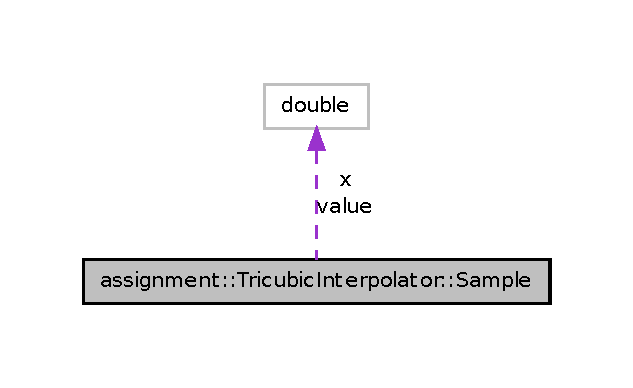
\includegraphics[width=304pt]{structassignment_1_1_tricubic_interpolator_1_1_sample__coll__graph}
\end{center}
\end{figure}
\subsection*{Public Attributes}
\begin{DoxyCompactItemize}
\item 
\hypertarget{structassignment_1_1_tricubic_interpolator_1_1_sample_a859e3262a400f13ee9142961b740bf99}{
double {\bfseries x}}
\label{structassignment_1_1_tricubic_interpolator_1_1_sample_a859e3262a400f13ee9142961b740bf99}

\item 
\hypertarget{structassignment_1_1_tricubic_interpolator_1_1_sample_a19eb3045df3e68721eae31ea2179d284}{
double {\bfseries value}}
\label{structassignment_1_1_tricubic_interpolator_1_1_sample_a19eb3045df3e68721eae31ea2179d284}

\end{DoxyCompactItemize}


The documentation for this struct was generated from the following file:\begin{DoxyCompactItemize}
\item 
assignment/TricubicInterpolator.h\end{DoxyCompactItemize}

\hypertarget{classassignment_1_1_trilinear_interpolator}{
\section{assignment::TrilinearInterpolator Class Reference}
\label{classassignment_1_1_trilinear_interpolator}\index{assignment::TrilinearInterpolator@{assignment::TrilinearInterpolator}}
}


Interpolates a \hyperlink{structmesh_1_1_mesh_1_1_point}{mesh::Mesh::Point} trilinear.  




{\ttfamily \#include $<$TrilinearInterpolator.h$>$}



Inheritance diagram for assignment::TrilinearInterpolator:\nopagebreak
\begin{figure}[H]
\begin{center}
\leavevmode
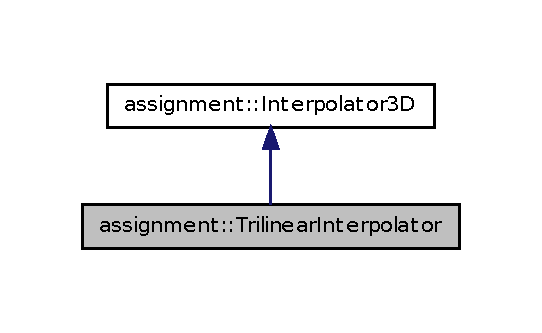
\includegraphics[width=260pt]{classassignment_1_1_trilinear_interpolator__inherit__graph}
\end{center}
\end{figure}


Collaboration diagram for assignment::TrilinearInterpolator:\nopagebreak
\begin{figure}[H]
\begin{center}
\leavevmode
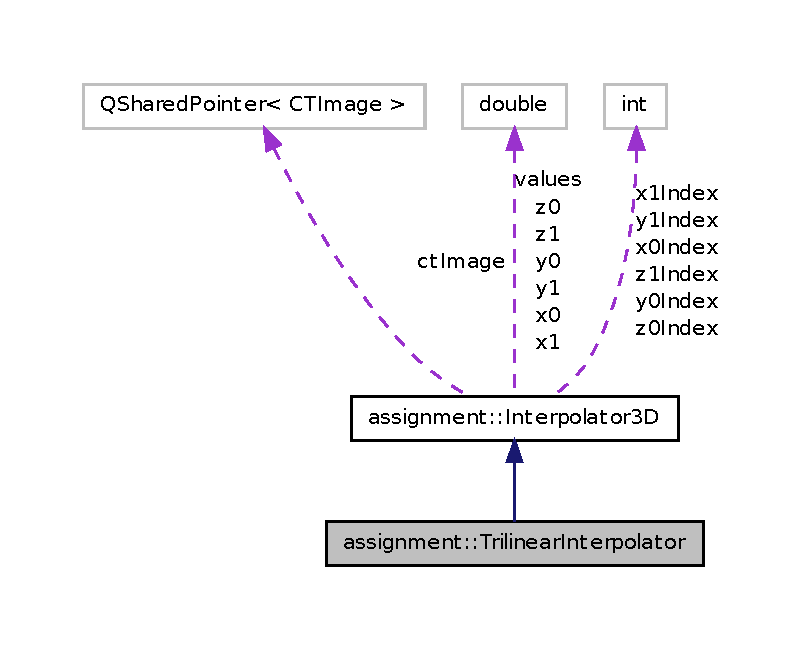
\includegraphics[width=385pt]{classassignment_1_1_trilinear_interpolator__coll__graph}
\end{center}
\end{figure}
\subsection*{Public Member Functions}
\begin{DoxyCompactItemize}
\item 
\hyperlink{classassignment_1_1_trilinear_interpolator_adbce93cb66d09622a5bde9fd51541783}{TrilinearInterpolator} (QSharedPointer$<$ \hyperlink{classctimage_1_1_c_t_image}{CTImage} $>$, double $\ast$)
\begin{DoxyCompactList}\small\item\em Creates a new trilinear interpolator with a given \hyperlink{classctimage_1_1_c_t_image}{ctimage::CTImage} and the values used for the interpolation. \item\end{DoxyCompactList}\item 
double \hyperlink{classassignment_1_1_trilinear_interpolator_a0972e2f1ebd828b832e94760c34b80c6}{getValue} (\hyperlink{structmesh_1_1_mesh_1_1_point}{Mesh::Point} $\ast$)
\begin{DoxyCompactList}\small\item\em Gets the interpolated value for a specified \hyperlink{structmesh_1_1_mesh_1_1_point}{mesh::Mesh::Point}. \item\end{DoxyCompactList}\end{DoxyCompactItemize}
\subsection*{Private Member Functions}
\begin{DoxyCompactItemize}
\item 
double \hyperlink{classassignment_1_1_trilinear_interpolator_a1b3999fc976f482b1ea41159a1170cd7}{interpolate} (double \hyperlink{classassignment_1_1_interpolator3_d_afb656ddf8789b483a8570f7a93985c0c}{x0}, double \hyperlink{classassignment_1_1_interpolator3_d_ab8f3111100189b5730621f77fe54467e}{x1}, double v0, double v1, double x)
\begin{DoxyCompactList}\small\item\em Returns the result of linear interpolation between two points. \item\end{DoxyCompactList}\end{DoxyCompactItemize}


\subsection{Detailed Description}
Interpolates a \hyperlink{structmesh_1_1_mesh_1_1_point}{mesh::Mesh::Point} trilinear. \begin{DoxyNote}{Note}
\href{http://en.wikipedia.org/wiki/Trilinear_interpolation}{\tt http://en.wikipedia.org/wiki/Trilinear\_\-interpolation} 
\end{DoxyNote}


\subsection{Constructor \& Destructor Documentation}
\hypertarget{classassignment_1_1_trilinear_interpolator_adbce93cb66d09622a5bde9fd51541783}{
\index{assignment::TrilinearInterpolator@{assignment::TrilinearInterpolator}!TrilinearInterpolator@{TrilinearInterpolator}}
\index{TrilinearInterpolator@{TrilinearInterpolator}!assignment::TrilinearInterpolator@{assignment::TrilinearInterpolator}}
\subsubsection[{TrilinearInterpolator}]{\setlength{\rightskip}{0pt plus 5cm}assignment::TrilinearInterpolator::TrilinearInterpolator (
\begin{DoxyParamCaption}
\item[{QSharedPointer$<$ {\bf CTImage} $>$}]{ ctImage, }
\item[{double $\ast$}]{ values}
\end{DoxyParamCaption}
)}}
\label{classassignment_1_1_trilinear_interpolator_adbce93cb66d09622a5bde9fd51541783}


Creates a new trilinear interpolator with a given \hyperlink{classctimage_1_1_c_t_image}{ctimage::CTImage} and the values used for the interpolation. 


\begin{DoxyParams}{Parameters}
\item[{\em ctImage}]The \hyperlink{classctimage_1_1_c_t_image}{ctimage::CTImage}, which is used only for morphologic information. The values of the \hyperlink{classctimage_1_1_c_t_image}{ctimage::CTImage} are not used for the interpolation \item[{\em values}]The values used for the interpolation. The values array needs to be the size of the pixel count of the \hyperlink{classctimage_1_1_c_t_image}{ctimage::CTImage} \end{DoxyParams}


\subsection{Member Function Documentation}
\hypertarget{classassignment_1_1_trilinear_interpolator_a0972e2f1ebd828b832e94760c34b80c6}{
\index{assignment::TrilinearInterpolator@{assignment::TrilinearInterpolator}!getValue@{getValue}}
\index{getValue@{getValue}!assignment::TrilinearInterpolator@{assignment::TrilinearInterpolator}}
\subsubsection[{getValue}]{\setlength{\rightskip}{0pt plus 5cm}double assignment::TrilinearInterpolator::getValue (
\begin{DoxyParamCaption}
\item[{{\bf Mesh::Point} $\ast$}]{ p}
\end{DoxyParamCaption}
)\hspace{0.3cm}{\ttfamily  \mbox{[}virtual\mbox{]}}}}
\label{classassignment_1_1_trilinear_interpolator_a0972e2f1ebd828b832e94760c34b80c6}


Gets the interpolated value for a specified \hyperlink{structmesh_1_1_mesh_1_1_point}{mesh::Mesh::Point}. 


\begin{DoxyParams}{Parameters}
\item[{\em p}]The point to be interpolated \end{DoxyParams}


Implements \hyperlink{classassignment_1_1_interpolator3_d_ac6ed5447418b7980d5ad2f12e853b35f}{assignment::Interpolator3D}.

\hypertarget{classassignment_1_1_trilinear_interpolator_a1b3999fc976f482b1ea41159a1170cd7}{
\index{assignment::TrilinearInterpolator@{assignment::TrilinearInterpolator}!interpolate@{interpolate}}
\index{interpolate@{interpolate}!assignment::TrilinearInterpolator@{assignment::TrilinearInterpolator}}
\subsubsection[{interpolate}]{\setlength{\rightskip}{0pt plus 5cm}double assignment::TrilinearInterpolator::interpolate (
\begin{DoxyParamCaption}
\item[{double}]{ x0, }
\item[{double}]{ x1, }
\item[{double}]{ v0, }
\item[{double}]{ v1, }
\item[{double}]{ x}
\end{DoxyParamCaption}
)\hspace{0.3cm}{\ttfamily  \mbox{[}private\mbox{]}}}}
\label{classassignment_1_1_trilinear_interpolator_a1b3999fc976f482b1ea41159a1170cd7}


Returns the result of linear interpolation between two points. 


\begin{DoxyParams}{Parameters}
\item[{\em x0}]The first sample point's coordinate \item[{\em x1}]The second sample point's coordinate \item[{\em v0}]The first sample point's value \item[{\em v1}]The second sample point's value \item[{\em x}]The coordinate of the point to be interpolated \end{DoxyParams}
\begin{DoxyReturn}{Returns}
The interpolation result 
\end{DoxyReturn}


The documentation for this class was generated from the following files:\begin{DoxyCompactItemize}
\item 
assignment/TrilinearInterpolator.h\item 
assignment/TrilinearInterpolator.cxx\end{DoxyCompactItemize}

\hypertarget{classcommand_1_1_parameter_parser}{
\section{command::ParameterParser Class Reference}
\label{classcommand_1_1_parameter_parser}\index{command::ParameterParser@{command::ParameterParser}}
}


Parses user input parameters.  




{\ttfamily \#include $<$ParameterParser.h$>$}



Collaboration diagram for command::ParameterParser:\nopagebreak
\begin{figure}[H]
\begin{center}
\leavevmode
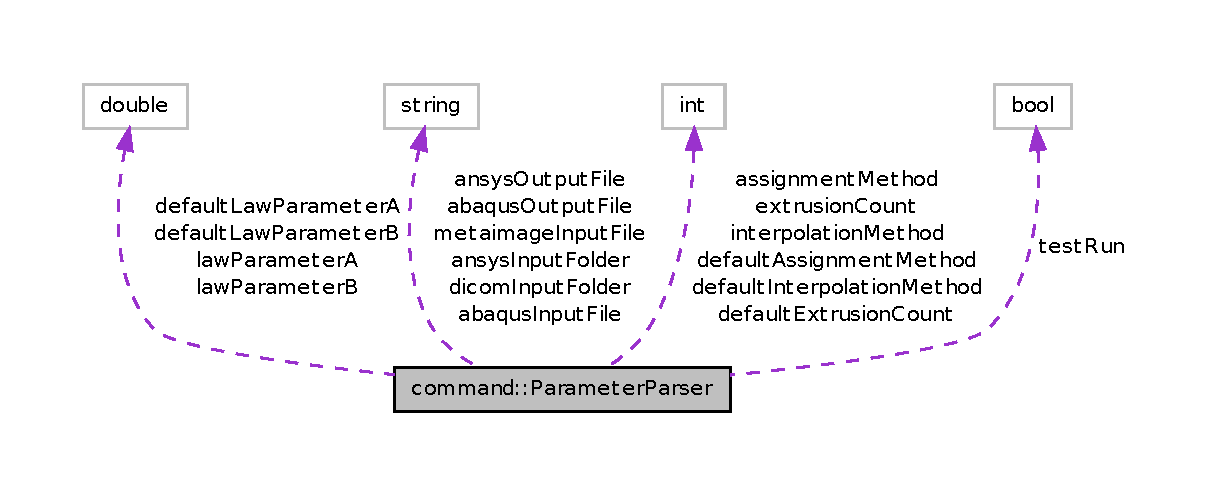
\includegraphics[width=400pt]{classcommand_1_1_parameter_parser__coll__graph}
\end{center}
\end{figure}
\subsection*{Public Member Functions}
\begin{DoxyCompactItemize}
\item 
string \hyperlink{classcommand_1_1_parameter_parser_a746a12b36f0881225c568f0b23bf815b}{parse} (int argc, char $\ast$$\ast$argv)
\begin{DoxyCompactList}\small\item\em Parses an array of program parameters. \item\end{DoxyCompactList}\item 
string \hyperlink{classcommand_1_1_parameter_parser_ae9cc20f77e2e0cb841d9f332604818ea}{parse} (char $\ast$arg)
\begin{DoxyCompactList}\small\item\em Parses a single parameter. \item\end{DoxyCompactList}\item 
bool \hyperlink{classcommand_1_1_parameter_parser_a0157d4dc3d92e25713da3d8a1855ce13}{getTestRun} ()
\begin{DoxyCompactList}\small\item\em Returns true if the tests will to be executed. \item\end{DoxyCompactList}\item 
int \hyperlink{classcommand_1_1_parameter_parser_a616ed93ea17dcae575e95684c461361c}{getExtrusionCount} ()
\begin{DoxyCompactList}\small\item\em Returns the number of extrusion iterations in the CT image extrusion. \item\end{DoxyCompactList}\item 
int \hyperlink{classcommand_1_1_parameter_parser_a391f0a5a9172660d42ab0aa0335aa7a3}{getInterpolationMethod} ()
\begin{DoxyCompactList}\small\item\em Returns the interpolation method. \item\end{DoxyCompactList}\item 
int \hyperlink{classcommand_1_1_parameter_parser_a1537acdf02c84c8d72d1bd7c48a491fc}{getAssignmentMethod} ()
\begin{DoxyCompactList}\small\item\em Returns the assignment method. \item\end{DoxyCompactList}\item 
string \hyperlink{classcommand_1_1_parameter_parser_afe39700e6cbaf3c08042cb2ad0a665f9}{getAbaqusInputFile} ()
\begin{DoxyCompactList}\small\item\em Returns the Abaqus input file. \item\end{DoxyCompactList}\item 
string \hyperlink{classcommand_1_1_parameter_parser_ae49c945fa67ed139c54679c636dc6e82}{getAnsysInputFolder} ()
\begin{DoxyCompactList}\small\item\em Returns the Ansys input folder. \item\end{DoxyCompactList}\item 
string \hyperlink{classcommand_1_1_parameter_parser_a24f467a6aad45d1dbb7b0b80b238c6dd}{getDicomInputFolder} ()
\begin{DoxyCompactList}\small\item\em Returns the Dicom input folder. \item\end{DoxyCompactList}\item 
string \hyperlink{classcommand_1_1_parameter_parser_abaf5fed7dedf9f2c4155cee75041321d}{getMetaimageInputFile} ()
\begin{DoxyCompactList}\small\item\em Returns the Abaqus input file. \item\end{DoxyCompactList}\item 
string \hyperlink{classcommand_1_1_parameter_parser_a6e4c59f60f04b2a25b940a1ab27c8734}{getAbaqusOutputFile} ()
\begin{DoxyCompactList}\small\item\em Returns the Abaqus file destination. \item\end{DoxyCompactList}\item 
string \hyperlink{classcommand_1_1_parameter_parser_adedfc9af8c5993e4b3776231b093faf9}{getAnsysOutputFile} ()
\begin{DoxyCompactList}\small\item\em Returns the Ansys file destination. \item\end{DoxyCompactList}\item 
double \hyperlink{classcommand_1_1_parameter_parser_ad69cf3bdc259377f6c65e2de8ae7fb4f}{getLawParameterA} ()
\begin{DoxyCompactList}\small\item\em Gets the first parameter for the assignment law. \item\end{DoxyCompactList}\item 
double \hyperlink{classcommand_1_1_parameter_parser_aa14baf15782ee89164d535bffa975bf9}{getLawParameterB} ()
\begin{DoxyCompactList}\small\item\em Gets the second parameter for the assignment law. \item\end{DoxyCompactList}\end{DoxyCompactItemize}
\subsection*{Private Member Functions}
\begin{DoxyCompactItemize}
\item 
\hypertarget{classcommand_1_1_parameter_parser_a2833fc94c1688934898c7b079684d45a}{
void \hyperlink{classcommand_1_1_parameter_parser_a2833fc94c1688934898c7b079684d45a}{setDefaultValues} ()}
\label{classcommand_1_1_parameter_parser_a2833fc94c1688934898c7b079684d45a}

\begin{DoxyCompactList}\small\item\em Set the values to a default state. \item\end{DoxyCompactList}\item 
string \hyperlink{classcommand_1_1_parameter_parser_a7a1cce7b6754b4ce4aba2540f01b40bb}{getHelpString} ()
\begin{DoxyCompactList}\small\item\em Gets the help output to be displayed the user. \item\end{DoxyCompactList}\end{DoxyCompactItemize}
\subsection*{Private Attributes}
\begin{DoxyCompactItemize}
\item 
\hypertarget{classcommand_1_1_parameter_parser_a234649998e2c18fbb8d47bde6c1f1ba7}{
int \hyperlink{classcommand_1_1_parameter_parser_a234649998e2c18fbb8d47bde6c1f1ba7}{interpolationMethod}}
\label{classcommand_1_1_parameter_parser_a234649998e2c18fbb8d47bde6c1f1ba7}

\begin{DoxyCompactList}\small\item\em The method for the interpolation Either assignment::TRILINEAR\_\-INTERPOLATION or assignment::TRICUBIC\_\-INTERPOLATION. \item\end{DoxyCompactList}\item 
\hypertarget{classcommand_1_1_parameter_parser_a1bcc6f566e71ca9a8cfba54d81dbc625}{
int \hyperlink{classcommand_1_1_parameter_parser_a1bcc6f566e71ca9a8cfba54d81dbc625}{extrusionCount}}
\label{classcommand_1_1_parameter_parser_a1bcc6f566e71ca9a8cfba54d81dbc625}

\begin{DoxyCompactList}\small\item\em The number of iterations for the CT image extrusion. \item\end{DoxyCompactList}\item 
\hypertarget{classcommand_1_1_parameter_parser_a62f598530edbad20d02e0ea5d3918f39}{
int \hyperlink{classcommand_1_1_parameter_parser_a62f598530edbad20d02e0ea5d3918f39}{assignmentMethod}}
\label{classcommand_1_1_parameter_parser_a62f598530edbad20d02e0ea5d3918f39}

\begin{DoxyCompactList}\small\item\em The method for the assignment Either assignment::NODE\_\-ASSIGNMENT or assignment::ELEMENT\_\-ASSIGNMENT. \item\end{DoxyCompactList}\item 
\hypertarget{classcommand_1_1_parameter_parser_ac67cdcc0339a96d20fb6c05fcc167ebf}{
bool \hyperlink{classcommand_1_1_parameter_parser_ac67cdcc0339a96d20fb6c05fcc167ebf}{testRun}}
\label{classcommand_1_1_parameter_parser_ac67cdcc0339a96d20fb6c05fcc167ebf}

\begin{DoxyCompactList}\small\item\em True if the tests will to be executed. \item\end{DoxyCompactList}\item 
\hypertarget{classcommand_1_1_parameter_parser_a38434d241d76f58223707fe17c4f8643}{
string \hyperlink{classcommand_1_1_parameter_parser_a38434d241d76f58223707fe17c4f8643}{abaqusInputFile}}
\label{classcommand_1_1_parameter_parser_a38434d241d76f58223707fe17c4f8643}

\begin{DoxyCompactList}\small\item\em The Abaqus input file. \item\end{DoxyCompactList}\item 
\hypertarget{classcommand_1_1_parameter_parser_a6e04e6d3ad9ee951912c6950eee46f05}{
string \hyperlink{classcommand_1_1_parameter_parser_a6e04e6d3ad9ee951912c6950eee46f05}{ansysInputFolder}}
\label{classcommand_1_1_parameter_parser_a6e04e6d3ad9ee951912c6950eee46f05}

\begin{DoxyCompactList}\small\item\em The Ansys input folder. \item\end{DoxyCompactList}\item 
\hypertarget{classcommand_1_1_parameter_parser_ac0fc0517f313841d224322e7c9f6297f}{
string \hyperlink{classcommand_1_1_parameter_parser_ac0fc0517f313841d224322e7c9f6297f}{dicomInputFolder}}
\label{classcommand_1_1_parameter_parser_ac0fc0517f313841d224322e7c9f6297f}

\begin{DoxyCompactList}\small\item\em The Dicom input folder. \item\end{DoxyCompactList}\item 
\hypertarget{classcommand_1_1_parameter_parser_a75d4cd4a63dbb299642a0d32af3e1e3c}{
string \hyperlink{classcommand_1_1_parameter_parser_a75d4cd4a63dbb299642a0d32af3e1e3c}{metaimageInputFile}}
\label{classcommand_1_1_parameter_parser_a75d4cd4a63dbb299642a0d32af3e1e3c}

\begin{DoxyCompactList}\small\item\em The Metaimage input file. \item\end{DoxyCompactList}\item 
\hypertarget{classcommand_1_1_parameter_parser_ace3041da862283468130afae6f8a6ef9}{
string \hyperlink{classcommand_1_1_parameter_parser_ace3041da862283468130afae6f8a6ef9}{abaqusOutputFile}}
\label{classcommand_1_1_parameter_parser_ace3041da862283468130afae6f8a6ef9}

\begin{DoxyCompactList}\small\item\em The Abaqus file for the export. \item\end{DoxyCompactList}\item 
\hypertarget{classcommand_1_1_parameter_parser_a658f1b9e13a618cde707c39d9c3fa47f}{
string \hyperlink{classcommand_1_1_parameter_parser_a658f1b9e13a618cde707c39d9c3fa47f}{ansysOutputFile}}
\label{classcommand_1_1_parameter_parser_a658f1b9e13a618cde707c39d9c3fa47f}

\begin{DoxyCompactList}\small\item\em The Ansys file for the export. \item\end{DoxyCompactList}\item 
\hypertarget{classcommand_1_1_parameter_parser_a509fd72437ab207b5e49b2181e9fe1cf}{
double \hyperlink{classcommand_1_1_parameter_parser_a509fd72437ab207b5e49b2181e9fe1cf}{lawParameterA}}
\label{classcommand_1_1_parameter_parser_a509fd72437ab207b5e49b2181e9fe1cf}

\begin{DoxyCompactList}\small\item\em The first parameter for the assignment law. \item\end{DoxyCompactList}\item 
\hypertarget{classcommand_1_1_parameter_parser_ab6e1cd89701906fb6b1da41615ea87b2}{
double \hyperlink{classcommand_1_1_parameter_parser_ab6e1cd89701906fb6b1da41615ea87b2}{lawParameterB}}
\label{classcommand_1_1_parameter_parser_ab6e1cd89701906fb6b1da41615ea87b2}

\begin{DoxyCompactList}\small\item\em The second parameter for the assignment law. \item\end{DoxyCompactList}\item 
\hypertarget{classcommand_1_1_parameter_parser_a58c087ec1d535bea3c441f21954e78c2}{
double \hyperlink{classcommand_1_1_parameter_parser_a58c087ec1d535bea3c441f21954e78c2}{defaultLawParameterA}}
\label{classcommand_1_1_parameter_parser_a58c087ec1d535bea3c441f21954e78c2}

\begin{DoxyCompactList}\small\item\em Default value for lawParameterA. \item\end{DoxyCompactList}\item 
\hypertarget{classcommand_1_1_parameter_parser_aca38ca87afb3329e1d610c92bf50b1d6}{
double \hyperlink{classcommand_1_1_parameter_parser_aca38ca87afb3329e1d610c92bf50b1d6}{defaultLawParameterB}}
\label{classcommand_1_1_parameter_parser_aca38ca87afb3329e1d610c92bf50b1d6}

\begin{DoxyCompactList}\small\item\em Default value for lawParameterB. \item\end{DoxyCompactList}\end{DoxyCompactItemize}
\subsection*{Static Private Attributes}
\begin{DoxyCompactItemize}
\item 
\hypertarget{classcommand_1_1_parameter_parser_ac15a30464e62c3505577b585ef975ed9}{
static const int \hyperlink{classcommand_1_1_parameter_parser_ac15a30464e62c3505577b585ef975ed9}{defaultExtrusionCount} = 3}
\label{classcommand_1_1_parameter_parser_ac15a30464e62c3505577b585ef975ed9}

\begin{DoxyCompactList}\small\item\em Default value for extrusionCount. \item\end{DoxyCompactList}\item 
\hypertarget{classcommand_1_1_parameter_parser_a99f702ccb0b934b9fa80f28ff5b78480}{
static const int \hyperlink{classcommand_1_1_parameter_parser_a99f702ccb0b934b9fa80f28ff5b78480}{defaultInterpolationMethod} = assignment::TRILINEAR\_\-INTERPOLATION}
\label{classcommand_1_1_parameter_parser_a99f702ccb0b934b9fa80f28ff5b78480}

\begin{DoxyCompactList}\small\item\em Default value for interpolationMethod. \item\end{DoxyCompactList}\item 
\hypertarget{classcommand_1_1_parameter_parser_a5e26fd646039c484fd61461074654e43}{
static const int \hyperlink{classcommand_1_1_parameter_parser_a5e26fd646039c484fd61461074654e43}{defaultAssignmentMethod} = assignment::NODE\_\-ASSIGNMENT}
\label{classcommand_1_1_parameter_parser_a5e26fd646039c484fd61461074654e43}

\begin{DoxyCompactList}\small\item\em Default value for assignmentMethod. \item\end{DoxyCompactList}\end{DoxyCompactItemize}


\subsection{Detailed Description}
Parses user input parameters. 

\subsection{Member Function Documentation}
\hypertarget{classcommand_1_1_parameter_parser_afe39700e6cbaf3c08042cb2ad0a665f9}{
\index{command::ParameterParser@{command::ParameterParser}!getAbaqusInputFile@{getAbaqusInputFile}}
\index{getAbaqusInputFile@{getAbaqusInputFile}!command::ParameterParser@{command::ParameterParser}}
\subsubsection[{getAbaqusInputFile}]{\setlength{\rightskip}{0pt plus 5cm}string command::ParameterParser::getAbaqusInputFile (
\begin{DoxyParamCaption}
{}
\end{DoxyParamCaption}
)}}
\label{classcommand_1_1_parameter_parser_afe39700e6cbaf3c08042cb2ad0a665f9}


Returns the Abaqus input file. 

\begin{DoxyReturn}{Returns}
The file location 
\end{DoxyReturn}
\hypertarget{classcommand_1_1_parameter_parser_a6e4c59f60f04b2a25b940a1ab27c8734}{
\index{command::ParameterParser@{command::ParameterParser}!getAbaqusOutputFile@{getAbaqusOutputFile}}
\index{getAbaqusOutputFile@{getAbaqusOutputFile}!command::ParameterParser@{command::ParameterParser}}
\subsubsection[{getAbaqusOutputFile}]{\setlength{\rightskip}{0pt plus 5cm}string command::ParameterParser::getAbaqusOutputFile (
\begin{DoxyParamCaption}
{}
\end{DoxyParamCaption}
)}}
\label{classcommand_1_1_parameter_parser_a6e4c59f60f04b2a25b940a1ab27c8734}


Returns the Abaqus file destination. 

\begin{DoxyReturn}{Returns}
The file destination 
\end{DoxyReturn}
\hypertarget{classcommand_1_1_parameter_parser_ae49c945fa67ed139c54679c636dc6e82}{
\index{command::ParameterParser@{command::ParameterParser}!getAnsysInputFolder@{getAnsysInputFolder}}
\index{getAnsysInputFolder@{getAnsysInputFolder}!command::ParameterParser@{command::ParameterParser}}
\subsubsection[{getAnsysInputFolder}]{\setlength{\rightskip}{0pt plus 5cm}string command::ParameterParser::getAnsysInputFolder (
\begin{DoxyParamCaption}
{}
\end{DoxyParamCaption}
)}}
\label{classcommand_1_1_parameter_parser_ae49c945fa67ed139c54679c636dc6e82}


Returns the Ansys input folder. 

\begin{DoxyReturn}{Returns}
The folder location 
\end{DoxyReturn}
\hypertarget{classcommand_1_1_parameter_parser_adedfc9af8c5993e4b3776231b093faf9}{
\index{command::ParameterParser@{command::ParameterParser}!getAnsysOutputFile@{getAnsysOutputFile}}
\index{getAnsysOutputFile@{getAnsysOutputFile}!command::ParameterParser@{command::ParameterParser}}
\subsubsection[{getAnsysOutputFile}]{\setlength{\rightskip}{0pt plus 5cm}string command::ParameterParser::getAnsysOutputFile (
\begin{DoxyParamCaption}
{}
\end{DoxyParamCaption}
)}}
\label{classcommand_1_1_parameter_parser_adedfc9af8c5993e4b3776231b093faf9}


Returns the Ansys file destination. 

\begin{DoxyReturn}{Returns}
The file destination 
\end{DoxyReturn}
\hypertarget{classcommand_1_1_parameter_parser_a1537acdf02c84c8d72d1bd7c48a491fc}{
\index{command::ParameterParser@{command::ParameterParser}!getAssignmentMethod@{getAssignmentMethod}}
\index{getAssignmentMethod@{getAssignmentMethod}!command::ParameterParser@{command::ParameterParser}}
\subsubsection[{getAssignmentMethod}]{\setlength{\rightskip}{0pt plus 5cm}int command::ParameterParser::getAssignmentMethod (
\begin{DoxyParamCaption}
{}
\end{DoxyParamCaption}
)}}
\label{classcommand_1_1_parameter_parser_a1537acdf02c84c8d72d1bd7c48a491fc}


Returns the assignment method. 

\begin{DoxyReturn}{Returns}
assignment::NODE\_\-ASSIGNMENT or assignment::ELEMENT\_\-ASSIGNMENT 
\end{DoxyReturn}
\hypertarget{classcommand_1_1_parameter_parser_a24f467a6aad45d1dbb7b0b80b238c6dd}{
\index{command::ParameterParser@{command::ParameterParser}!getDicomInputFolder@{getDicomInputFolder}}
\index{getDicomInputFolder@{getDicomInputFolder}!command::ParameterParser@{command::ParameterParser}}
\subsubsection[{getDicomInputFolder}]{\setlength{\rightskip}{0pt plus 5cm}string command::ParameterParser::getDicomInputFolder (
\begin{DoxyParamCaption}
{}
\end{DoxyParamCaption}
)}}
\label{classcommand_1_1_parameter_parser_a24f467a6aad45d1dbb7b0b80b238c6dd}


Returns the Dicom input folder. 

\begin{DoxyReturn}{Returns}
The folder location 
\end{DoxyReturn}
\hypertarget{classcommand_1_1_parameter_parser_a616ed93ea17dcae575e95684c461361c}{
\index{command::ParameterParser@{command::ParameterParser}!getExtrusionCount@{getExtrusionCount}}
\index{getExtrusionCount@{getExtrusionCount}!command::ParameterParser@{command::ParameterParser}}
\subsubsection[{getExtrusionCount}]{\setlength{\rightskip}{0pt plus 5cm}int command::ParameterParser::getExtrusionCount (
\begin{DoxyParamCaption}
{}
\end{DoxyParamCaption}
)}}
\label{classcommand_1_1_parameter_parser_a616ed93ea17dcae575e95684c461361c}


Returns the number of extrusion iterations in the CT image extrusion. 

\begin{DoxyReturn}{Returns}
The number of extrusion iterations 
\end{DoxyReturn}
\hypertarget{classcommand_1_1_parameter_parser_a7a1cce7b6754b4ce4aba2540f01b40bb}{
\index{command::ParameterParser@{command::ParameterParser}!getHelpString@{getHelpString}}
\index{getHelpString@{getHelpString}!command::ParameterParser@{command::ParameterParser}}
\subsubsection[{getHelpString}]{\setlength{\rightskip}{0pt plus 5cm}string command::ParameterParser::getHelpString (
\begin{DoxyParamCaption}
{}
\end{DoxyParamCaption}
)\hspace{0.3cm}{\ttfamily  \mbox{[}private\mbox{]}}}}
\label{classcommand_1_1_parameter_parser_a7a1cce7b6754b4ce4aba2540f01b40bb}


Gets the help output to be displayed the user. 

\begin{DoxyReturn}{Returns}
The help output 
\end{DoxyReturn}
\hypertarget{classcommand_1_1_parameter_parser_a391f0a5a9172660d42ab0aa0335aa7a3}{
\index{command::ParameterParser@{command::ParameterParser}!getInterpolationMethod@{getInterpolationMethod}}
\index{getInterpolationMethod@{getInterpolationMethod}!command::ParameterParser@{command::ParameterParser}}
\subsubsection[{getInterpolationMethod}]{\setlength{\rightskip}{0pt plus 5cm}int command::ParameterParser::getInterpolationMethod (
\begin{DoxyParamCaption}
{}
\end{DoxyParamCaption}
)}}
\label{classcommand_1_1_parameter_parser_a391f0a5a9172660d42ab0aa0335aa7a3}


Returns the interpolation method. 

\begin{DoxyReturn}{Returns}
assignment::TRILINEAR\_\-INTERPOLATION or assignment::TRICUBIC\_\-INTERPOLATION 
\end{DoxyReturn}
\hypertarget{classcommand_1_1_parameter_parser_ad69cf3bdc259377f6c65e2de8ae7fb4f}{
\index{command::ParameterParser@{command::ParameterParser}!getLawParameterA@{getLawParameterA}}
\index{getLawParameterA@{getLawParameterA}!command::ParameterParser@{command::ParameterParser}}
\subsubsection[{getLawParameterA}]{\setlength{\rightskip}{0pt plus 5cm}double command::ParameterParser::getLawParameterA (
\begin{DoxyParamCaption}
{}
\end{DoxyParamCaption}
)}}
\label{classcommand_1_1_parameter_parser_ad69cf3bdc259377f6c65e2de8ae7fb4f}


Gets the first parameter for the assignment law. 

\begin{DoxyReturn}{Returns}
The first law assignment parameter 
\end{DoxyReturn}
\hypertarget{classcommand_1_1_parameter_parser_aa14baf15782ee89164d535bffa975bf9}{
\index{command::ParameterParser@{command::ParameterParser}!getLawParameterB@{getLawParameterB}}
\index{getLawParameterB@{getLawParameterB}!command::ParameterParser@{command::ParameterParser}}
\subsubsection[{getLawParameterB}]{\setlength{\rightskip}{0pt plus 5cm}double command::ParameterParser::getLawParameterB (
\begin{DoxyParamCaption}
{}
\end{DoxyParamCaption}
)}}
\label{classcommand_1_1_parameter_parser_aa14baf15782ee89164d535bffa975bf9}


Gets the second parameter for the assignment law. 

\begin{DoxyReturn}{Returns}
The second law assignment parameter 
\end{DoxyReturn}
\hypertarget{classcommand_1_1_parameter_parser_abaf5fed7dedf9f2c4155cee75041321d}{
\index{command::ParameterParser@{command::ParameterParser}!getMetaimageInputFile@{getMetaimageInputFile}}
\index{getMetaimageInputFile@{getMetaimageInputFile}!command::ParameterParser@{command::ParameterParser}}
\subsubsection[{getMetaimageInputFile}]{\setlength{\rightskip}{0pt plus 5cm}string command::ParameterParser::getMetaimageInputFile (
\begin{DoxyParamCaption}
{}
\end{DoxyParamCaption}
)}}
\label{classcommand_1_1_parameter_parser_abaf5fed7dedf9f2c4155cee75041321d}


Returns the Abaqus input file. 

\begin{DoxyReturn}{Returns}
The file location 
\end{DoxyReturn}
\hypertarget{classcommand_1_1_parameter_parser_a0157d4dc3d92e25713da3d8a1855ce13}{
\index{command::ParameterParser@{command::ParameterParser}!getTestRun@{getTestRun}}
\index{getTestRun@{getTestRun}!command::ParameterParser@{command::ParameterParser}}
\subsubsection[{getTestRun}]{\setlength{\rightskip}{0pt plus 5cm}bool command::ParameterParser::getTestRun (
\begin{DoxyParamCaption}
{}
\end{DoxyParamCaption}
)}}
\label{classcommand_1_1_parameter_parser_a0157d4dc3d92e25713da3d8a1855ce13}


Returns true if the tests will to be executed. 

\begin{DoxyReturn}{Returns}
Whether the tests will be executed 
\end{DoxyReturn}
\hypertarget{classcommand_1_1_parameter_parser_a746a12b36f0881225c568f0b23bf815b}{
\index{command::ParameterParser@{command::ParameterParser}!parse@{parse}}
\index{parse@{parse}!command::ParameterParser@{command::ParameterParser}}
\subsubsection[{parse}]{\setlength{\rightskip}{0pt plus 5cm}string command::ParameterParser::parse (
\begin{DoxyParamCaption}
\item[{int}]{ argc, }
\item[{char $\ast$$\ast$}]{ argv}
\end{DoxyParamCaption}
)}}
\label{classcommand_1_1_parameter_parser_a746a12b36f0881225c568f0b23bf815b}


Parses an array of program parameters. 

\begin{DoxyWarning}{Warning}
The first value in the char array is ignored as it usually contains the program's name 
\end{DoxyWarning}

\begin{DoxyParams}{Parameters}
\item[{\em argc}]The parameter count \item[{\em argv}]The parameter array \end{DoxyParams}
\begin{DoxyReturn}{Returns}
The error message. If the return string is empty the parsing was successful 
\end{DoxyReturn}
\hypertarget{classcommand_1_1_parameter_parser_ae9cc20f77e2e0cb841d9f332604818ea}{
\index{command::ParameterParser@{command::ParameterParser}!parse@{parse}}
\index{parse@{parse}!command::ParameterParser@{command::ParameterParser}}
\subsubsection[{parse}]{\setlength{\rightskip}{0pt plus 5cm}string command::ParameterParser::parse (
\begin{DoxyParamCaption}
\item[{char $\ast$}]{ arg}
\end{DoxyParamCaption}
)}}
\label{classcommand_1_1_parameter_parser_ae9cc20f77e2e0cb841d9f332604818ea}


Parses a single parameter. 


\begin{DoxyParams}{Parameters}
\item[{\em arg}]A parameter \end{DoxyParams}
\begin{DoxyReturn}{Returns}
The error message. If the return string is empty the parsing was successful 
\end{DoxyReturn}


The documentation for this class was generated from the following files:\begin{DoxyCompactItemize}
\item 
command/ParameterParser.h\item 
command/ParameterParser.cxx\end{DoxyCompactItemize}

\hypertarget{classcommand_1_1_runner}{
\section{command::Runner Class Reference}
\label{classcommand_1_1_runner}\index{command::Runner@{command::Runner}}
}


Runs the application in command line mode.  




{\ttfamily \#include $<$Runner.h$>$}



Collaboration diagram for command::Runner:\nopagebreak
\begin{figure}[H]
\begin{center}
\leavevmode
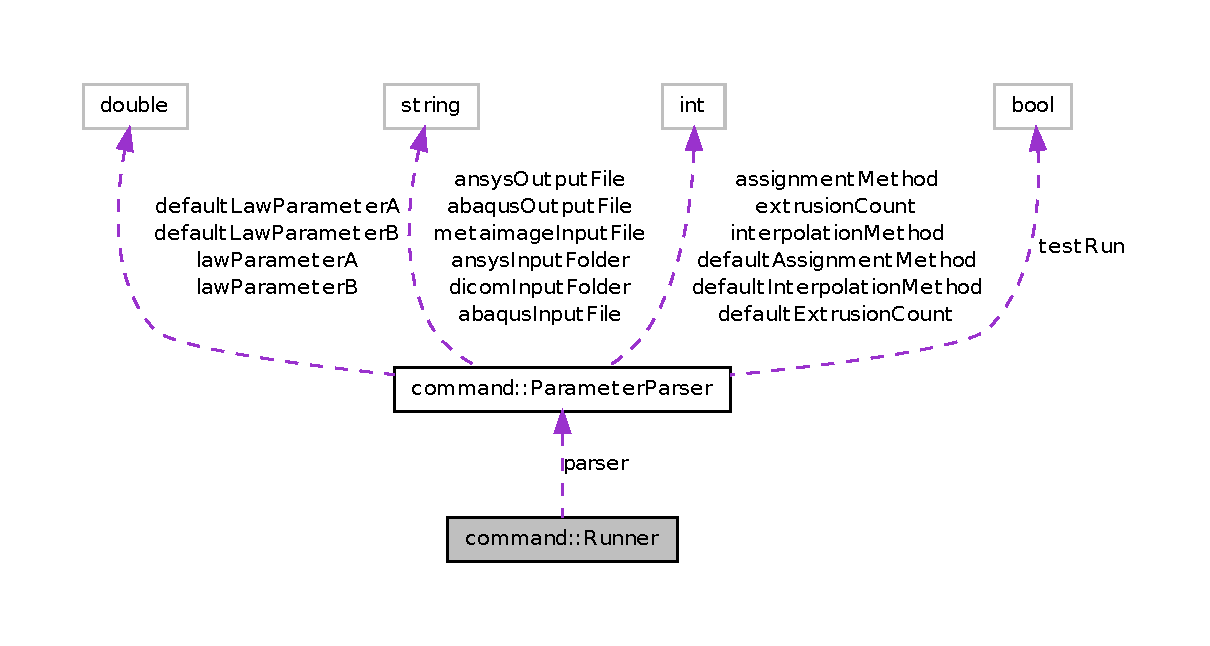
\includegraphics[width=400pt]{classcommand_1_1_runner__coll__graph}
\end{center}
\end{figure}
\subsection*{Public Member Functions}
\begin{DoxyCompactItemize}
\item 
\hyperlink{classcommand_1_1_runner_afe9efc7e2b8ba3ffd9dce513342f0a46}{Runner} (int argc, char $\ast$$\ast$argv)
\begin{DoxyCompactList}\small\item\em Constructs a \hyperlink{classcommand_1_1_runner}{Runner}. \item\end{DoxyCompactList}\item 
\hypertarget{classcommand_1_1_runner_a0d91edb3156141b1ff1a4ff7086a9711}{
void \hyperlink{classcommand_1_1_runner_a0d91edb3156141b1ff1a4ff7086a9711}{run} ()}
\label{classcommand_1_1_runner_a0d91edb3156141b1ff1a4ff7086a9711}

\begin{DoxyCompactList}\small\item\em Starts the application. \item\end{DoxyCompactList}\end{DoxyCompactItemize}
\subsection*{Private Attributes}
\begin{DoxyCompactItemize}
\item 
\hypertarget{classcommand_1_1_runner_aec623548d5c2c53fcb7b8eb5241c3435}{
\hyperlink{classcommand_1_1_parameter_parser}{ParameterParser} \hyperlink{classcommand_1_1_runner_aec623548d5c2c53fcb7b8eb5241c3435}{parser}}
\label{classcommand_1_1_runner_aec623548d5c2c53fcb7b8eb5241c3435}

\begin{DoxyCompactList}\small\item\em The parser for the user input parameters. \item\end{DoxyCompactList}\end{DoxyCompactItemize}


\subsection{Detailed Description}
Runs the application in command line mode. 

\subsection{Constructor \& Destructor Documentation}
\hypertarget{classcommand_1_1_runner_afe9efc7e2b8ba3ffd9dce513342f0a46}{
\index{command::Runner@{command::Runner}!Runner@{Runner}}
\index{Runner@{Runner}!command::Runner@{command::Runner}}
\subsubsection[{Runner}]{\setlength{\rightskip}{0pt plus 5cm}command::Runner::Runner (
\begin{DoxyParamCaption}
\item[{int}]{ argc, }
\item[{char $\ast$$\ast$}]{ argv}
\end{DoxyParamCaption}
)}}
\label{classcommand_1_1_runner_afe9efc7e2b8ba3ffd9dce513342f0a46}


Constructs a \hyperlink{classcommand_1_1_runner}{Runner}. 


\begin{DoxyParams}{Parameters}
\item[{\em argc}]The number of input parameters \item[{\em argv}]The input parameter array \end{DoxyParams}


The documentation for this class was generated from the following files:\begin{DoxyCompactItemize}
\item 
command/Runner.h\item 
command/Runner.cxx\end{DoxyCompactItemize}

\hypertarget{classctimage_1_1_c_t_image}{
\section{ctimage::CTImage Class Reference}
\label{classctimage_1_1_c_t_image}\index{ctimage::CTImage@{ctimage::CTImage}}
}


Inheritance diagram for ctimage::CTImage:\nopagebreak
\begin{figure}[H]
\begin{center}
\leavevmode
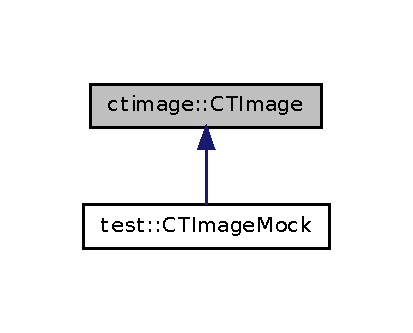
\includegraphics[width=198pt]{classctimage_1_1_c_t_image__inherit__graph}
\end{center}
\end{figure}


Collaboration diagram for ctimage::CTImage:\nopagebreak
\begin{figure}[H]
\begin{center}
\leavevmode
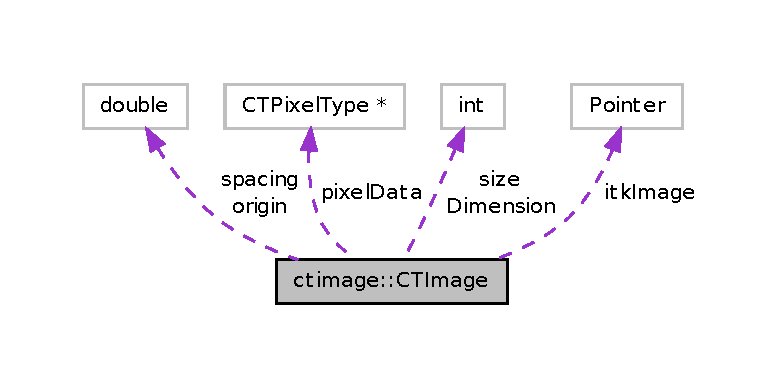
\includegraphics[width=375pt]{classctimage_1_1_c_t_image__coll__graph}
\end{center}
\end{figure}
\subsection*{Public Types}
\begin{DoxyCompactItemize}
\item 
\hypertarget{classctimage_1_1_c_t_image_ab3bf32a276d168a705973d8d6c698cec}{
typedef signed short \hyperlink{classctimage_1_1_c_t_image_ab3bf32a276d168a705973d8d6c698cec}{CTPixelType}}
\label{classctimage_1_1_c_t_image_ab3bf32a276d168a705973d8d6c698cec}

\begin{DoxyCompactList}\small\item\em The type of a CT pixel value. \item\end{DoxyCompactList}\item 
\hypertarget{classctimage_1_1_c_t_image_a6e3fc439772d8f22861508d9a7e3e694}{
typedef itk::Image$<$ \hyperlink{classctimage_1_1_c_t_image_ab3bf32a276d168a705973d8d6c698cec}{CTPixelType}, \hyperlink{classctimage_1_1_c_t_image_ad28aaad081539a4a2e7f1cc38c06aa3a}{Dimension} $>$ \hyperlink{classctimage_1_1_c_t_image_a6e3fc439772d8f22861508d9a7e3e694}{ItkImageType}}
\label{classctimage_1_1_c_t_image_a6e3fc439772d8f22861508d9a7e3e694}

\begin{DoxyCompactList}\small\item\em The type of an itk::Image. \item\end{DoxyCompactList}\end{DoxyCompactItemize}
\subsection*{Public Member Functions}
\begin{DoxyCompactItemize}
\item 
\hyperlink{classctimage_1_1_c_t_image_ab3bf32a276d168a705973d8d6c698cec}{CTPixelType} $\ast$ \hyperlink{classctimage_1_1_c_t_image_a6878ee1b7181be6227408fe453c8ac8b}{getPixelData} ()
\item 
int \hyperlink{classctimage_1_1_c_t_image_a877fb3bce920ba1bb352491c50b4d168}{getNx} ()
\item 
int \hyperlink{classctimage_1_1_c_t_image_a031a3229e2354a57490312c154c3b0db}{getNy} ()
\item 
int \hyperlink{classctimage_1_1_c_t_image_a005e1a22619e37ee6ed2515911e1ab1d}{getNz} ()
\item 
int \hyperlink{classctimage_1_1_c_t_image_a62f2e4428c651f31febc96b10f189632}{getNsum} ()
\item 
double \hyperlink{classctimage_1_1_c_t_image_a544abec0ed785ab4b42cccf11c59dc98}{getSx} ()
\item 
double \hyperlink{classctimage_1_1_c_t_image_aefac72b6ce49db1ce878103adbe9eb6a}{getSy} ()
\item 
double \hyperlink{classctimage_1_1_c_t_image_a26e2a9db85e602f43f2a86ae34504436}{getSz} ()
\item 
double \hyperlink{classctimage_1_1_c_t_image_ab1cae0aaaf707edb3b4dd1bb86093076}{getX0} ()
\item 
double \hyperlink{classctimage_1_1_c_t_image_a66a56ee2161af9eba00cff98cb2d07dd}{getY0} ()
\item 
double \hyperlink{classctimage_1_1_c_t_image_a6317b268b24347587a430adb34b767cb}{getZ0} ()
\item 
ItkImageType::Pointer \hyperlink{classctimage_1_1_c_t_image_a56db4348cfa2c01d80b9cfd4aea7ef73}{getItkImage} ()
\item 
QSharedPointer$<$ \hyperlink{classctimage_1_1_c_t_image}{CTImage} $>$ \hyperlink{classctimage_1_1_c_t_image_aa80c85e696bdad6bdeebad7c4ca01d76}{createDeepCopy} ()
\begin{DoxyCompactList}\small\item\em Creates a full copy of the CT image. \item\end{DoxyCompactList}\item 
void \hyperlink{classctimage_1_1_c_t_image_a3f3dfc3759b0fbdd2bc2eedffbe5546a}{write} (string)
\begin{DoxyCompactList}\small\item\em Writes the image in DICOM format to the disk. \item\end{DoxyCompactList}\end{DoxyCompactItemize}
\subsection*{Static Public Attributes}
\begin{DoxyCompactItemize}
\item 
\hypertarget{classctimage_1_1_c_t_image_ad28aaad081539a4a2e7f1cc38c06aa3a}{
static const int \hyperlink{classctimage_1_1_c_t_image_ad28aaad081539a4a2e7f1cc38c06aa3a}{Dimension} = 3}
\label{classctimage_1_1_c_t_image_ad28aaad081539a4a2e7f1cc38c06aa3a}

\begin{DoxyCompactList}\small\item\em The dimension of the CT image. \item\end{DoxyCompactList}\end{DoxyCompactItemize}
\subsection*{Protected Attributes}
\begin{DoxyCompactItemize}
\item 
\hypertarget{classctimage_1_1_c_t_image_af6d5d0c3991568e121f0543ebaad348c}{
\hyperlink{classctimage_1_1_c_t_image_ab3bf32a276d168a705973d8d6c698cec}{CTPixelType} $\ast$ \hyperlink{classctimage_1_1_c_t_image_af6d5d0c3991568e121f0543ebaad348c}{pixelData}}
\label{classctimage_1_1_c_t_image_af6d5d0c3991568e121f0543ebaad348c}

\begin{DoxyCompactList}\small\item\em Pixel data array. \item\end{DoxyCompactList}\item 
\hypertarget{classctimage_1_1_c_t_image_aab436b15c45aff941a30ebbf3d9ccd7f}{
int \hyperlink{classctimage_1_1_c_t_image_aab436b15c45aff941a30ebbf3d9ccd7f}{size} \mbox{[}\hyperlink{classctimage_1_1_c_t_image_ad28aaad081539a4a2e7f1cc38c06aa3a}{Dimension}\mbox{]}}
\label{classctimage_1_1_c_t_image_aab436b15c45aff941a30ebbf3d9ccd7f}

\begin{DoxyCompactList}\small\item\em The dimension in all (xyz) directions. \item\end{DoxyCompactList}\item 
\hypertarget{classctimage_1_1_c_t_image_ab9a73f002d0cb09bf5a5212f9d64d98f}{
double \hyperlink{classctimage_1_1_c_t_image_ab9a73f002d0cb09bf5a5212f9d64d98f}{spacing} \mbox{[}\hyperlink{classctimage_1_1_c_t_image_ad28aaad081539a4a2e7f1cc38c06aa3a}{Dimension}\mbox{]}}
\label{classctimage_1_1_c_t_image_ab9a73f002d0cb09bf5a5212f9d64d98f}

\begin{DoxyCompactList}\small\item\em The spacing between two pixels in all directions. \item\end{DoxyCompactList}\item 
\hypertarget{classctimage_1_1_c_t_image_ac021e29ecd42262c6a9db72b8b97ce13}{
double \hyperlink{classctimage_1_1_c_t_image_ac021e29ecd42262c6a9db72b8b97ce13}{origin} \mbox{[}\hyperlink{classctimage_1_1_c_t_image_ad28aaad081539a4a2e7f1cc38c06aa3a}{Dimension}\mbox{]}}
\label{classctimage_1_1_c_t_image_ac021e29ecd42262c6a9db72b8b97ce13}

\begin{DoxyCompactList}\small\item\em The position of the first pixel of each direction. \item\end{DoxyCompactList}\item 
\hypertarget{classctimage_1_1_c_t_image_a178d337fefde126244059e5b7f548f0f}{
ItkImageType::Pointer \hyperlink{classctimage_1_1_c_t_image_a178d337fefde126244059e5b7f548f0f}{itkImage}}
\label{classctimage_1_1_c_t_image_a178d337fefde126244059e5b7f548f0f}

\begin{DoxyCompactList}\small\item\em The itk::itkImage. \item\end{DoxyCompactList}\end{DoxyCompactItemize}
\subsection*{Friends}
\begin{DoxyCompactItemize}
\item 
\hypertarget{classctimage_1_1_c_t_image_a5cc1455156c67f189525c313a80fb9fc}{
class {\bfseries DicomCTImageReader}}
\label{classctimage_1_1_c_t_image_a5cc1455156c67f189525c313a80fb9fc}

\item 
\hypertarget{classctimage_1_1_c_t_image_a0966d000a96e20736d2debc5591acef1}{
class {\bfseries MetaimageCTImageReader}}
\label{classctimage_1_1_c_t_image_a0966d000a96e20736d2debc5591acef1}

\item 
\hypertarget{classctimage_1_1_c_t_image_ac136807d795545b8468400f61e1b95d2}{
class {\bfseries CTImageReader}}
\label{classctimage_1_1_c_t_image_ac136807d795545b8468400f61e1b95d2}

\end{DoxyCompactItemize}


\subsection{Member Function Documentation}
\hypertarget{classctimage_1_1_c_t_image_aa80c85e696bdad6bdeebad7c4ca01d76}{
\index{ctimage::CTImage@{ctimage::CTImage}!createDeepCopy@{createDeepCopy}}
\index{createDeepCopy@{createDeepCopy}!ctimage::CTImage@{ctimage::CTImage}}
\subsubsection[{createDeepCopy}]{\setlength{\rightskip}{0pt plus 5cm}QSharedPointer$<$ {\bf CTImage} $>$ ctimage::CTImage::createDeepCopy (
\begin{DoxyParamCaption}
{}
\end{DoxyParamCaption}
)}}
\label{classctimage_1_1_c_t_image_aa80c85e696bdad6bdeebad7c4ca01d76}


Creates a full copy of the CT image. 

\begin{DoxyReturn}{Returns}
Pointer to the duplicated \hyperlink{classctimage_1_1_c_t_image}{ctimage::CTImage} 
\end{DoxyReturn}
\hypertarget{classctimage_1_1_c_t_image_a56db4348cfa2c01d80b9cfd4aea7ef73}{
\index{ctimage::CTImage@{ctimage::CTImage}!getItkImage@{getItkImage}}
\index{getItkImage@{getItkImage}!ctimage::CTImage@{ctimage::CTImage}}
\subsubsection[{getItkImage}]{\setlength{\rightskip}{0pt plus 5cm}CTImage::ItkImageType::Pointer ctimage::CTImage::getItkImage (
\begin{DoxyParamCaption}
{}
\end{DoxyParamCaption}
)}}
\label{classctimage_1_1_c_t_image_a56db4348cfa2c01d80b9cfd4aea7ef73}
\begin{DoxyReturn}{Returns}
The itk::itkImage 
\end{DoxyReturn}
\hypertarget{classctimage_1_1_c_t_image_a62f2e4428c651f31febc96b10f189632}{
\index{ctimage::CTImage@{ctimage::CTImage}!getNsum@{getNsum}}
\index{getNsum@{getNsum}!ctimage::CTImage@{ctimage::CTImage}}
\subsubsection[{getNsum}]{\setlength{\rightskip}{0pt plus 5cm}int ctimage::CTImage::getNsum (
\begin{DoxyParamCaption}
{}
\end{DoxyParamCaption}
)}}
\label{classctimage_1_1_c_t_image_a62f2e4428c651f31febc96b10f189632}
\begin{DoxyReturn}{Returns}
Number of pixels in total 
\end{DoxyReturn}
\hypertarget{classctimage_1_1_c_t_image_a877fb3bce920ba1bb352491c50b4d168}{
\index{ctimage::CTImage@{ctimage::CTImage}!getNx@{getNx}}
\index{getNx@{getNx}!ctimage::CTImage@{ctimage::CTImage}}
\subsubsection[{getNx}]{\setlength{\rightskip}{0pt plus 5cm}int ctimage::CTImage::getNx (
\begin{DoxyParamCaption}
{}
\end{DoxyParamCaption}
)}}
\label{classctimage_1_1_c_t_image_a877fb3bce920ba1bb352491c50b4d168}
\begin{DoxyReturn}{Returns}
Number of pixels in x direction 
\end{DoxyReturn}
\hypertarget{classctimage_1_1_c_t_image_a031a3229e2354a57490312c154c3b0db}{
\index{ctimage::CTImage@{ctimage::CTImage}!getNy@{getNy}}
\index{getNy@{getNy}!ctimage::CTImage@{ctimage::CTImage}}
\subsubsection[{getNy}]{\setlength{\rightskip}{0pt plus 5cm}int ctimage::CTImage::getNy (
\begin{DoxyParamCaption}
{}
\end{DoxyParamCaption}
)}}
\label{classctimage_1_1_c_t_image_a031a3229e2354a57490312c154c3b0db}
\begin{DoxyReturn}{Returns}
Number of pixels in y direction 
\end{DoxyReturn}
\hypertarget{classctimage_1_1_c_t_image_a005e1a22619e37ee6ed2515911e1ab1d}{
\index{ctimage::CTImage@{ctimage::CTImage}!getNz@{getNz}}
\index{getNz@{getNz}!ctimage::CTImage@{ctimage::CTImage}}
\subsubsection[{getNz}]{\setlength{\rightskip}{0pt plus 5cm}int ctimage::CTImage::getNz (
\begin{DoxyParamCaption}
{}
\end{DoxyParamCaption}
)}}
\label{classctimage_1_1_c_t_image_a005e1a22619e37ee6ed2515911e1ab1d}
\begin{DoxyReturn}{Returns}
Number of pixels in z direction 
\end{DoxyReturn}
\hypertarget{classctimage_1_1_c_t_image_a6878ee1b7181be6227408fe453c8ac8b}{
\index{ctimage::CTImage@{ctimage::CTImage}!getPixelData@{getPixelData}}
\index{getPixelData@{getPixelData}!ctimage::CTImage@{ctimage::CTImage}}
\subsubsection[{getPixelData}]{\setlength{\rightskip}{0pt plus 5cm}{\bf CTImage::CTPixelType} $\ast$ ctimage::CTImage::getPixelData (
\begin{DoxyParamCaption}
{}
\end{DoxyParamCaption}
)}}
\label{classctimage_1_1_c_t_image_a6878ee1b7181be6227408fe453c8ac8b}
\begin{DoxyReturn}{Returns}
The CT image's pixels 
\end{DoxyReturn}
\hypertarget{classctimage_1_1_c_t_image_a544abec0ed785ab4b42cccf11c59dc98}{
\index{ctimage::CTImage@{ctimage::CTImage}!getSx@{getSx}}
\index{getSx@{getSx}!ctimage::CTImage@{ctimage::CTImage}}
\subsubsection[{getSx}]{\setlength{\rightskip}{0pt plus 5cm}double ctimage::CTImage::getSx (
\begin{DoxyParamCaption}
{}
\end{DoxyParamCaption}
)}}
\label{classctimage_1_1_c_t_image_a544abec0ed785ab4b42cccf11c59dc98}
\begin{DoxyReturn}{Returns}
Spacing between pixels in x direction 
\end{DoxyReturn}
\hypertarget{classctimage_1_1_c_t_image_aefac72b6ce49db1ce878103adbe9eb6a}{
\index{ctimage::CTImage@{ctimage::CTImage}!getSy@{getSy}}
\index{getSy@{getSy}!ctimage::CTImage@{ctimage::CTImage}}
\subsubsection[{getSy}]{\setlength{\rightskip}{0pt plus 5cm}double ctimage::CTImage::getSy (
\begin{DoxyParamCaption}
{}
\end{DoxyParamCaption}
)}}
\label{classctimage_1_1_c_t_image_aefac72b6ce49db1ce878103adbe9eb6a}
\begin{DoxyReturn}{Returns}
Spacing between pixels in y direction 
\end{DoxyReturn}
\hypertarget{classctimage_1_1_c_t_image_a26e2a9db85e602f43f2a86ae34504436}{
\index{ctimage::CTImage@{ctimage::CTImage}!getSz@{getSz}}
\index{getSz@{getSz}!ctimage::CTImage@{ctimage::CTImage}}
\subsubsection[{getSz}]{\setlength{\rightskip}{0pt plus 5cm}double ctimage::CTImage::getSz (
\begin{DoxyParamCaption}
{}
\end{DoxyParamCaption}
)}}
\label{classctimage_1_1_c_t_image_a26e2a9db85e602f43f2a86ae34504436}
\begin{DoxyReturn}{Returns}
Spacing between pixels in z direction 
\end{DoxyReturn}
\hypertarget{classctimage_1_1_c_t_image_ab1cae0aaaf707edb3b4dd1bb86093076}{
\index{ctimage::CTImage@{ctimage::CTImage}!getX0@{getX0}}
\index{getX0@{getX0}!ctimage::CTImage@{ctimage::CTImage}}
\subsubsection[{getX0}]{\setlength{\rightskip}{0pt plus 5cm}double ctimage::CTImage::getX0 (
\begin{DoxyParamCaption}
{}
\end{DoxyParamCaption}
)}}
\label{classctimage_1_1_c_t_image_ab1cae0aaaf707edb3b4dd1bb86093076}
\begin{DoxyReturn}{Returns}
The x-\/coordinate of the first pixel 
\end{DoxyReturn}
\hypertarget{classctimage_1_1_c_t_image_a66a56ee2161af9eba00cff98cb2d07dd}{
\index{ctimage::CTImage@{ctimage::CTImage}!getY0@{getY0}}
\index{getY0@{getY0}!ctimage::CTImage@{ctimage::CTImage}}
\subsubsection[{getY0}]{\setlength{\rightskip}{0pt plus 5cm}double ctimage::CTImage::getY0 (
\begin{DoxyParamCaption}
{}
\end{DoxyParamCaption}
)}}
\label{classctimage_1_1_c_t_image_a66a56ee2161af9eba00cff98cb2d07dd}
\begin{DoxyReturn}{Returns}
The y-\/coordinate of the first pixel 
\end{DoxyReturn}
\hypertarget{classctimage_1_1_c_t_image_a6317b268b24347587a430adb34b767cb}{
\index{ctimage::CTImage@{ctimage::CTImage}!getZ0@{getZ0}}
\index{getZ0@{getZ0}!ctimage::CTImage@{ctimage::CTImage}}
\subsubsection[{getZ0}]{\setlength{\rightskip}{0pt plus 5cm}double ctimage::CTImage::getZ0 (
\begin{DoxyParamCaption}
{}
\end{DoxyParamCaption}
)}}
\label{classctimage_1_1_c_t_image_a6317b268b24347587a430adb34b767cb}
\begin{DoxyReturn}{Returns}
The z-\/coordinate of the first pixel 
\end{DoxyReturn}
\hypertarget{classctimage_1_1_c_t_image_a3f3dfc3759b0fbdd2bc2eedffbe5546a}{
\index{ctimage::CTImage@{ctimage::CTImage}!write@{write}}
\index{write@{write}!ctimage::CTImage@{ctimage::CTImage}}
\subsubsection[{write}]{\setlength{\rightskip}{0pt plus 5cm}void ctimage::CTImage::write (
\begin{DoxyParamCaption}
\item[{string}]{ directory}
\end{DoxyParamCaption}
)}}
\label{classctimage_1_1_c_t_image_a3f3dfc3759b0fbdd2bc2eedffbe5546a}


Writes the image in DICOM format to the disk. 


\begin{DoxyParams}{Parameters}
\item[{\em The}]destination folder \end{DoxyParams}


The documentation for this class was generated from the following files:\begin{DoxyCompactItemize}
\item 
ctimage/CTImage.h\item 
ctimage/CTImage.cxx\end{DoxyCompactItemize}

\hypertarget{classctimage_1_1_c_t_image_reader}{
\section{ctimage::CTImageReader Class Reference}
\label{classctimage_1_1_c_t_image_reader}\index{ctimage::CTImageReader@{ctimage::CTImageReader}}
}


Reads a CT Image from disk.  




{\ttfamily \#include $<$CTImageReader.h$>$}



Inheritance diagram for ctimage::CTImageReader:\nopagebreak
\begin{figure}[H]
\begin{center}
\leavevmode
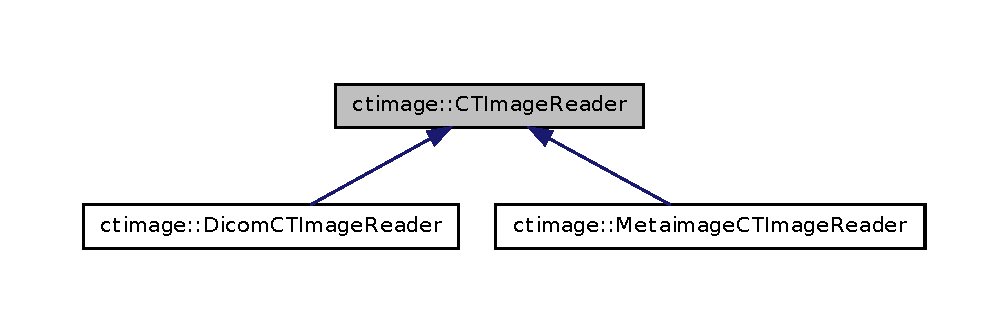
\includegraphics[width=400pt]{classctimage_1_1_c_t_image_reader__inherit__graph}
\end{center}
\end{figure}


Collaboration diagram for ctimage::CTImageReader:\nopagebreak
\begin{figure}[H]
\begin{center}
\leavevmode
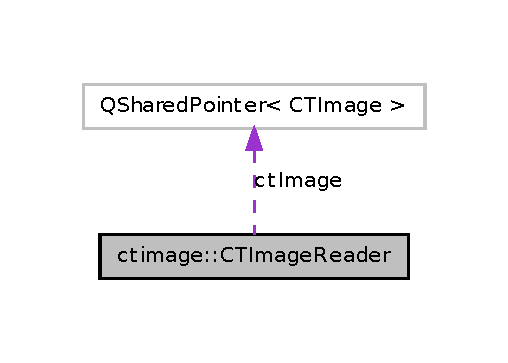
\includegraphics[width=244pt]{classctimage_1_1_c_t_image_reader__coll__graph}
\end{center}
\end{figure}
\subsection*{Public Member Functions}
\begin{DoxyCompactItemize}
\item 
QSharedPointer$<$ \hyperlink{classctimage_1_1_c_t_image}{CTImage} $>$ \hyperlink{classctimage_1_1_c_t_image_reader_a86ddbe900d2d0e7c4129dcd7380595dc}{getCtImage} ()
\end{DoxyCompactItemize}
\subsection*{Protected Member Functions}
\begin{DoxyCompactItemize}
\item 
\hypertarget{classctimage_1_1_c_t_image_reader_aa061965652a3eacf8a3d9a3f436a1495}{
void \hyperlink{classctimage_1_1_c_t_image_reader_aa061965652a3eacf8a3d9a3f436a1495}{setMetadata} ()}
\label{classctimage_1_1_c_t_image_reader_aa061965652a3eacf8a3d9a3f436a1495}

\begin{DoxyCompactList}\small\item\em Sets up ctImage's members holding the morphologic information of the image. \item\end{DoxyCompactList}\end{DoxyCompactItemize}
\subsection*{Protected Attributes}
\begin{DoxyCompactItemize}
\item 
\hypertarget{classctimage_1_1_c_t_image_reader_a15c76cbe2dfffac08c1a4f84463b5fc7}{
QSharedPointer$<$ \hyperlink{classctimage_1_1_c_t_image}{CTImage} $>$ \hyperlink{classctimage_1_1_c_t_image_reader_a15c76cbe2dfffac08c1a4f84463b5fc7}{ctImage}}
\label{classctimage_1_1_c_t_image_reader_a15c76cbe2dfffac08c1a4f84463b5fc7}

\begin{DoxyCompactList}\small\item\em The image which was read. \item\end{DoxyCompactList}\end{DoxyCompactItemize}


\subsection{Detailed Description}
Reads a CT Image from disk. 

\subsection{Member Function Documentation}
\hypertarget{classctimage_1_1_c_t_image_reader_a86ddbe900d2d0e7c4129dcd7380595dc}{
\index{ctimage::CTImageReader@{ctimage::CTImageReader}!getCtImage@{getCtImage}}
\index{getCtImage@{getCtImage}!ctimage::CTImageReader@{ctimage::CTImageReader}}
\subsubsection[{getCtImage}]{\setlength{\rightskip}{0pt plus 5cm}QSharedPointer$<$ {\bf CTImage} $>$ ctimage::CTImageReader::getCtImage (
\begin{DoxyParamCaption}
{}
\end{DoxyParamCaption}
)}}
\label{classctimage_1_1_c_t_image_reader_a86ddbe900d2d0e7c4129dcd7380595dc}
\begin{DoxyReturn}{Returns}
The image which was read 
\end{DoxyReturn}


The documentation for this class was generated from the following files:\begin{DoxyCompactItemize}
\item 
ctimage/CTImageReader.h\item 
ctimage/CTImageReader.cxx\end{DoxyCompactItemize}

\hypertarget{classctimage_1_1_dicom_c_t_image_reader}{
\section{ctimage::DicomCTImageReader Class Reference}
\label{classctimage_1_1_dicom_c_t_image_reader}\index{ctimage::DicomCTImageReader@{ctimage::DicomCTImageReader}}
}


Reads a image stack in DICOM format.  




{\ttfamily \#include $<$DicomCTImageReader.h$>$}



Inheritance diagram for ctimage::DicomCTImageReader:\nopagebreak
\begin{figure}[H]
\begin{center}
\leavevmode
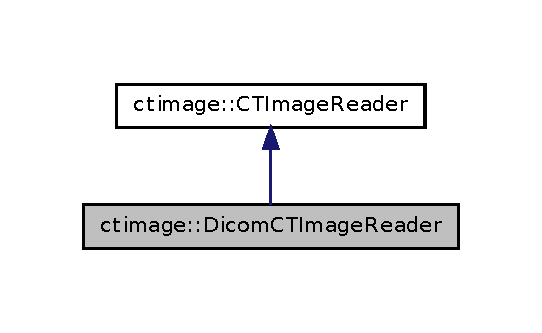
\includegraphics[width=260pt]{classctimage_1_1_dicom_c_t_image_reader__inherit__graph}
\end{center}
\end{figure}


Collaboration diagram for ctimage::DicomCTImageReader:\nopagebreak
\begin{figure}[H]
\begin{center}
\leavevmode
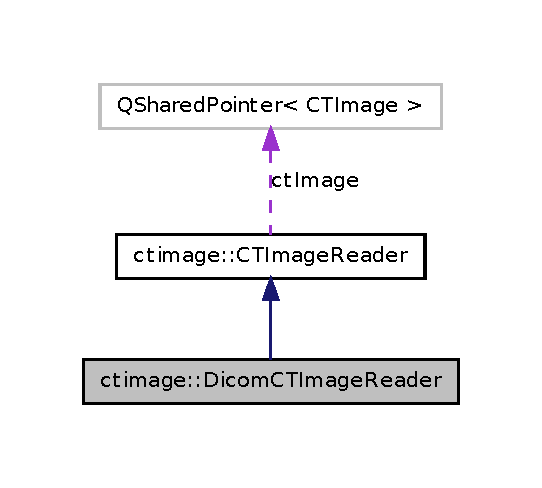
\includegraphics[width=260pt]{classctimage_1_1_dicom_c_t_image_reader__coll__graph}
\end{center}
\end{figure}
\subsection*{Public Member Functions}
\begin{DoxyCompactItemize}
\item 
\hyperlink{classctimage_1_1_dicom_c_t_image_reader_ae687ff251a2f1b13e12a2362ff552662}{DicomCTImageReader} (string)
\begin{DoxyCompactList}\small\item\em Creates a new DICOM reader and reads the image. \item\end{DoxyCompactList}\end{DoxyCompactItemize}


\subsection{Detailed Description}
Reads a image stack in DICOM format. 

\subsection{Constructor \& Destructor Documentation}
\hypertarget{classctimage_1_1_dicom_c_t_image_reader_ae687ff251a2f1b13e12a2362ff552662}{
\index{ctimage::DicomCTImageReader@{ctimage::DicomCTImageReader}!DicomCTImageReader@{DicomCTImageReader}}
\index{DicomCTImageReader@{DicomCTImageReader}!ctimage::DicomCTImageReader@{ctimage::DicomCTImageReader}}
\subsubsection[{DicomCTImageReader}]{\setlength{\rightskip}{0pt plus 5cm}ctimage::DicomCTImageReader::DicomCTImageReader (
\begin{DoxyParamCaption}
\item[{string}]{ directory}
\end{DoxyParamCaption}
)}}
\label{classctimage_1_1_dicom_c_t_image_reader_ae687ff251a2f1b13e12a2362ff552662}


Creates a new DICOM reader and reads the image. 


\begin{DoxyParams}{Parameters}
\item[{\em The}]folder containing the DICOM stack \end{DoxyParams}


The documentation for this class was generated from the following files:\begin{DoxyCompactItemize}
\item 
ctimage/DicomCTImageReader.h\item 
ctimage/DicomCTImageReader.cxx\end{DoxyCompactItemize}

\hypertarget{classctimage_1_1_metaimage_c_t_image_reader}{
\section{ctimage::MetaimageCTImageReader Class Reference}
\label{classctimage_1_1_metaimage_c_t_image_reader}\index{ctimage::MetaimageCTImageReader@{ctimage::MetaimageCTImageReader}}
}


Reads a CT image in Metaimage fomat from disk.  




{\ttfamily \#include $<$MetaimageCTImageReader.h$>$}



Inheritance diagram for ctimage::MetaimageCTImageReader:\nopagebreak
\begin{figure}[H]
\begin{center}
\leavevmode
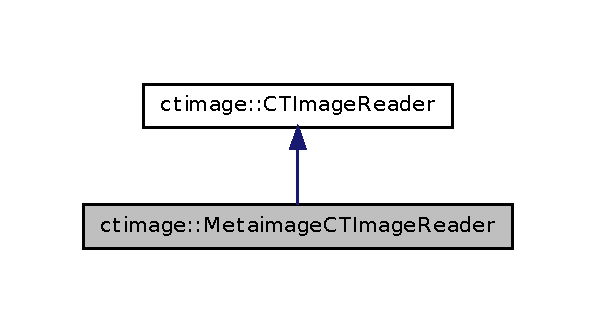
\includegraphics[width=286pt]{classctimage_1_1_metaimage_c_t_image_reader__inherit__graph}
\end{center}
\end{figure}


Collaboration diagram for ctimage::MetaimageCTImageReader:\nopagebreak
\begin{figure}[H]
\begin{center}
\leavevmode
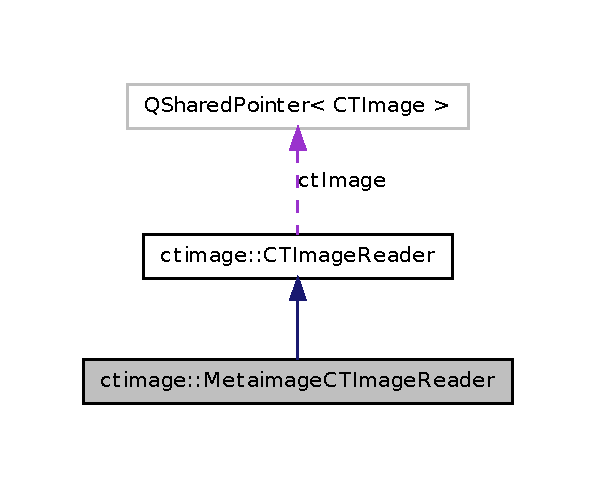
\includegraphics[width=286pt]{classctimage_1_1_metaimage_c_t_image_reader__coll__graph}
\end{center}
\end{figure}
\subsection*{Public Member Functions}
\begin{DoxyCompactItemize}
\item 
\hyperlink{classctimage_1_1_metaimage_c_t_image_reader_a55bd18bbac70258c8ba8885b55532bb3}{MetaimageCTImageReader} (string)
\begin{DoxyCompactList}\small\item\em Creates a Metaimage reader and reads the specified file. \item\end{DoxyCompactList}\end{DoxyCompactItemize}


\subsection{Detailed Description}
Reads a CT image in Metaimage fomat from disk. 

\subsection{Constructor \& Destructor Documentation}
\hypertarget{classctimage_1_1_metaimage_c_t_image_reader_a55bd18bbac70258c8ba8885b55532bb3}{
\index{ctimage::MetaimageCTImageReader@{ctimage::MetaimageCTImageReader}!MetaimageCTImageReader@{MetaimageCTImageReader}}
\index{MetaimageCTImageReader@{MetaimageCTImageReader}!ctimage::MetaimageCTImageReader@{ctimage::MetaimageCTImageReader}}
\subsubsection[{MetaimageCTImageReader}]{\setlength{\rightskip}{0pt plus 5cm}ctimage::MetaimageCTImageReader::MetaimageCTImageReader (
\begin{DoxyParamCaption}
\item[{string}]{ filename}
\end{DoxyParamCaption}
)}}
\label{classctimage_1_1_metaimage_c_t_image_reader_a55bd18bbac70258c8ba8885b55532bb3}


Creates a Metaimage reader and reads the specified file. 


\begin{DoxyParams}{Parameters}
\item[{\em The}]Metaimage file location \end{DoxyParams}


The documentation for this class was generated from the following files:\begin{DoxyCompactItemize}
\item 
ctimage/MetaimageCTImageReader.h\item 
ctimage/MetaimageCTImageReader.cxx\end{DoxyCompactItemize}

\hypertarget{classctimage_1_1_volume_corrector}{
\section{ctimage::VolumeCorrector Class Reference}
\label{classctimage_1_1_volume_corrector}\index{ctimage::VolumeCorrector@{ctimage::VolumeCorrector}}
}


Extrudes a \hyperlink{classctimage_1_1_c_t_image}{ctimage::CTImage} in order to completely cover a \hyperlink{classmesh_1_1_mesh}{mesh::Mesh}.  




{\ttfamily \#include $<$VolumeCorrector.h$>$}



Collaboration diagram for ctimage::VolumeCorrector:\nopagebreak
\begin{figure}[H]
\begin{center}
\leavevmode
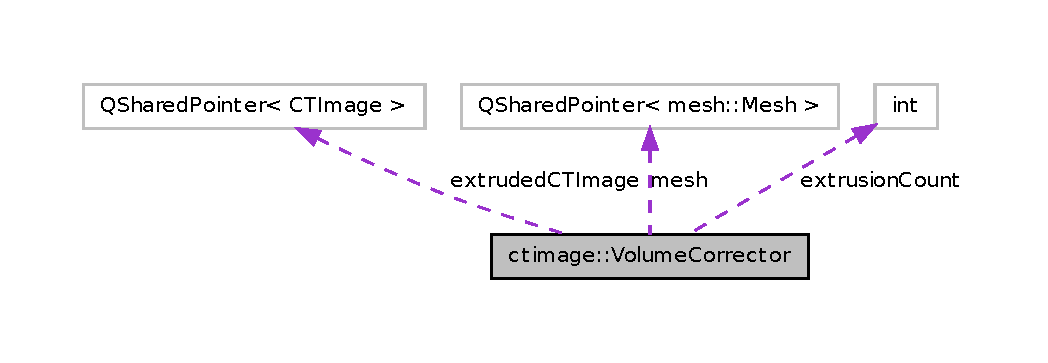
\includegraphics[width=400pt]{classctimage_1_1_volume_corrector__coll__graph}
\end{center}
\end{figure}
\subsection*{Classes}
\begin{DoxyCompactItemize}
\item 
struct \hyperlink{structctimage_1_1_volume_corrector_1_1_line}{Line}
\begin{DoxyCompactList}\small\item\em A connection of two points. \item\end{DoxyCompactList}\item 
struct \hyperlink{structctimage_1_1_volume_corrector_1_1_point2_d}{Point2D}
\begin{DoxyCompactList}\small\item\em A 2-\/Dimensional point. \item\end{DoxyCompactList}\end{DoxyCompactItemize}
\subsection*{Public Member Functions}
\begin{DoxyCompactItemize}
\item 
\hyperlink{classctimage_1_1_volume_corrector_a38ceb67dfbd2ff41d8c87c1c5853a3b3}{VolumeCorrector} (QSharedPointer$<$ \hyperlink{classctimage_1_1_c_t_image}{CTImage} $>$ ctImage, QSharedPointer$<$ \hyperlink{classmesh_1_1_mesh}{mesh::Mesh} $>$ \hyperlink{classctimage_1_1_volume_corrector_a619b8444da48d717b5314a04b39fc6cd}{mesh}, int)
\item 
QSharedPointer$<$ \hyperlink{classctimage_1_1_c_t_image}{CTImage} $>$ \hyperlink{classctimage_1_1_volume_corrector_ae7766967e85dd56a1e0809fd75365557}{getExtrudedCTImage} ()
\begin{DoxyCompactList}\small\item\em Returns the extruded \hyperlink{classctimage_1_1_c_t_image}{ctimage::CTImage}. \item\end{DoxyCompactList}\end{DoxyCompactItemize}
\subsection*{Private Member Functions}
\begin{DoxyCompactItemize}
\item 
\hypertarget{classctimage_1_1_volume_corrector_ae1891b19fec618b507d20b5578e75b72}{
void \hyperlink{classctimage_1_1_volume_corrector_ae1891b19fec618b507d20b5578e75b72}{extrude} ()}
\label{classctimage_1_1_volume_corrector_ae1891b19fec618b507d20b5578e75b72}

\begin{DoxyCompactList}\small\item\em Run the extrusion routine. \item\end{DoxyCompactList}\item 
void \hyperlink{classctimage_1_1_volume_corrector_ac596c5e63de666f0c12459f7c473d14e}{inTetrahedron} (bool $\ast$)
\begin{DoxyCompactList}\small\item\em Fills a bool array which is true where the points are inside a tetrahedron. \item\end{DoxyCompactList}\item 
\hypertarget{classctimage_1_1_volume_corrector_a060febb7b26980a6075f37b5c119cd8e}{
void {\bfseries chopSurface} (bool $\ast$ctBool, bool $\ast$ctSlim, bool $\ast$ctPeeled)}
\label{classctimage_1_1_volume_corrector_a060febb7b26980a6075f37b5c119cd8e}

\item 
\hypertarget{classctimage_1_1_volume_corrector_a55b87ef81e929c87b8b0c46e4cc4cc62}{
void {\bfseries extendSurface} (\hyperlink{classctimage_1_1_c_t_image_ab3bf32a276d168a705973d8d6c698cec}{CTImage::CTPixelType} $\ast$E, bool $\ast$c, \hyperlink{classctimage_1_1_c_t_image_ab3bf32a276d168a705973d8d6c698cec}{CTImage::CTPixelType} $\ast$Ex, bool $\ast$cx)}
\label{classctimage_1_1_volume_corrector_a55b87ef81e929c87b8b0c46e4cc4cc62}

\end{DoxyCompactItemize}
\subsection*{Private Attributes}
\begin{DoxyCompactItemize}
\item 
\hypertarget{classctimage_1_1_volume_corrector_ad58e1281952791cc0508ba7e531d335a}{
int \hyperlink{classctimage_1_1_volume_corrector_ad58e1281952791cc0508ba7e531d335a}{extrusionCount}}
\label{classctimage_1_1_volume_corrector_ad58e1281952791cc0508ba7e531d335a}

\begin{DoxyCompactList}\small\item\em The iteration count for the image extrusion. \item\end{DoxyCompactList}\item 
\hypertarget{classctimage_1_1_volume_corrector_a619b8444da48d717b5314a04b39fc6cd}{
QSharedPointer$<$ \hyperlink{classmesh_1_1_mesh}{mesh::Mesh} $>$ \hyperlink{classctimage_1_1_volume_corrector_a619b8444da48d717b5314a04b39fc6cd}{mesh}}
\label{classctimage_1_1_volume_corrector_a619b8444da48d717b5314a04b39fc6cd}

\begin{DoxyCompactList}\small\item\em The mesh that corresponds to the specified \hyperlink{classctimage_1_1_c_t_image}{ctimage::CTImage}. \item\end{DoxyCompactList}\item 
\hypertarget{classctimage_1_1_volume_corrector_aeba98b07c027b1d9c1e8d6219aaee468}{
QSharedPointer$<$ \hyperlink{classctimage_1_1_c_t_image}{CTImage} $>$ \hyperlink{classctimage_1_1_volume_corrector_aeba98b07c027b1d9c1e8d6219aaee468}{extrudedCTImage}}
\label{classctimage_1_1_volume_corrector_aeba98b07c027b1d9c1e8d6219aaee468}

\begin{DoxyCompactList}\small\item\em The extruded \hyperlink{classctimage_1_1_c_t_image}{ctimage::CTImage}. \item\end{DoxyCompactList}\end{DoxyCompactItemize}


\subsection{Detailed Description}
Extrudes a \hyperlink{classctimage_1_1_c_t_image}{ctimage::CTImage} in order to completely cover a \hyperlink{classmesh_1_1_mesh}{mesh::Mesh}. \begin{DoxyWarning}{Warning}
This class doesn't alter the provided \hyperlink{classctimage_1_1_c_t_image}{ctimage::CTImage}. It instead creates a new \hyperlink{classctimage_1_1_c_t_image}{ctimage::CTImage} 
\end{DoxyWarning}


\subsection{Constructor \& Destructor Documentation}
\hypertarget{classctimage_1_1_volume_corrector_a38ceb67dfbd2ff41d8c87c1c5853a3b3}{
\index{ctimage::VolumeCorrector@{ctimage::VolumeCorrector}!VolumeCorrector@{VolumeCorrector}}
\index{VolumeCorrector@{VolumeCorrector}!ctimage::VolumeCorrector@{ctimage::VolumeCorrector}}
\subsubsection[{VolumeCorrector}]{\setlength{\rightskip}{0pt plus 5cm}ctimage::VolumeCorrector::VolumeCorrector (
\begin{DoxyParamCaption}
\item[{QSharedPointer$<$ {\bf CTImage} $>$}]{ ctImage, }
\item[{QSharedPointer$<$ {\bf mesh::Mesh} $>$}]{ mesh, }
\item[{int}]{ extrusionCount}
\end{DoxyParamCaption}
)}}
\label{classctimage_1_1_volume_corrector_a38ceb67dfbd2ff41d8c87c1c5853a3b3}

\begin{DoxyParams}{Parameters}
\item[{\em ctImage}]The \hyperlink{classctimage_1_1_c_t_image}{ctimage::CTImage} to be extruded \item[{\em mesh}]The corresponding \hyperlink{classmesh_1_1_mesh}{mesh::Mesh} \end{DoxyParams}


\subsection{Member Function Documentation}
\hypertarget{classctimage_1_1_volume_corrector_ae7766967e85dd56a1e0809fd75365557}{
\index{ctimage::VolumeCorrector@{ctimage::VolumeCorrector}!getExtrudedCTImage@{getExtrudedCTImage}}
\index{getExtrudedCTImage@{getExtrudedCTImage}!ctimage::VolumeCorrector@{ctimage::VolumeCorrector}}
\subsubsection[{getExtrudedCTImage}]{\setlength{\rightskip}{0pt plus 5cm}QSharedPointer$<$ {\bf CTImage} $>$ ctimage::VolumeCorrector::getExtrudedCTImage (
\begin{DoxyParamCaption}
{}
\end{DoxyParamCaption}
)}}
\label{classctimage_1_1_volume_corrector_ae7766967e85dd56a1e0809fd75365557}


Returns the extruded \hyperlink{classctimage_1_1_c_t_image}{ctimage::CTImage}. 

\begin{DoxyReturn}{Returns}
The extruded \hyperlink{classctimage_1_1_c_t_image}{ctimage::CTImage} 
\end{DoxyReturn}
\hypertarget{classctimage_1_1_volume_corrector_ac596c5e63de666f0c12459f7c473d14e}{
\index{ctimage::VolumeCorrector@{ctimage::VolumeCorrector}!inTetrahedron@{inTetrahedron}}
\index{inTetrahedron@{inTetrahedron}!ctimage::VolumeCorrector@{ctimage::VolumeCorrector}}
\subsubsection[{inTetrahedron}]{\setlength{\rightskip}{0pt plus 5cm}void ctimage::VolumeCorrector::inTetrahedron (
\begin{DoxyParamCaption}
\item[{bool $\ast$}]{ ctBool}
\end{DoxyParamCaption}
)\hspace{0.3cm}{\ttfamily  \mbox{[}private\mbox{]}}}}
\label{classctimage_1_1_volume_corrector_ac596c5e63de666f0c12459f7c473d14e}


Fills a bool array which is true where the points are inside a tetrahedron. 


\begin{DoxyParams}{Parameters}
\item[{\em The}]bool array that will be filled \end{DoxyParams}
\begin{DoxyWarning}{Warning}
The bool array must be the size of the amount of pixels in the \hyperlink{classctimage_1_1_c_t_image}{ctimage::CTImage} 
\end{DoxyWarning}


The documentation for this class was generated from the following files:\begin{DoxyCompactItemize}
\item 
ctimage/VolumeCorrector.h\item 
ctimage/VolumeCorrector.cxx\end{DoxyCompactItemize}

\hypertarget{structctimage_1_1_volume_corrector_1_1_line}{
\section{ctimage::VolumeCorrector::Line Struct Reference}
\label{structctimage_1_1_volume_corrector_1_1_line}\index{ctimage::VolumeCorrector::Line@{ctimage::VolumeCorrector::Line}}
}


A connection of two points.  




Collaboration diagram for ctimage::VolumeCorrector::Line:\nopagebreak
\begin{figure}[H]
\begin{center}
\leavevmode
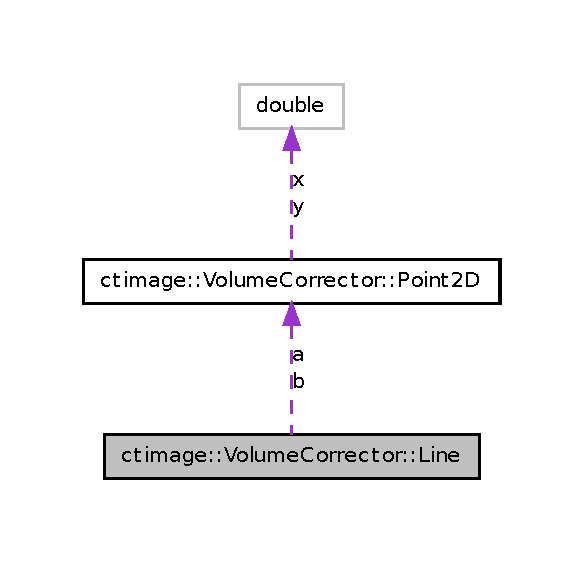
\includegraphics[width=280pt]{structctimage_1_1_volume_corrector_1_1_line__coll__graph}
\end{center}
\end{figure}
\subsection*{Public Attributes}
\begin{DoxyCompactItemize}
\item 
\hypertarget{structctimage_1_1_volume_corrector_1_1_line_aff84c86854913816c85a1928a2efcf71}{
\hyperlink{structctimage_1_1_volume_corrector_1_1_point2_d}{Point2D} {\bfseries a}}
\label{structctimage_1_1_volume_corrector_1_1_line_aff84c86854913816c85a1928a2efcf71}

\item 
\hypertarget{structctimage_1_1_volume_corrector_1_1_line_acc253a7ba87122fe96e270a23d220876}{
\hyperlink{structctimage_1_1_volume_corrector_1_1_point2_d}{Point2D} {\bfseries b}}
\label{structctimage_1_1_volume_corrector_1_1_line_acc253a7ba87122fe96e270a23d220876}

\end{DoxyCompactItemize}


\subsection{Detailed Description}
A connection of two points. 

The documentation for this struct was generated from the following file:\begin{DoxyCompactItemize}
\item 
ctimage/VolumeCorrector.h\end{DoxyCompactItemize}

\hypertarget{structctimage_1_1_volume_corrector_1_1_point2_d}{
\section{ctimage::VolumeCorrector::Point2D Struct Reference}
\label{structctimage_1_1_volume_corrector_1_1_point2_d}\index{ctimage::VolumeCorrector::Point2D@{ctimage::VolumeCorrector::Point2D}}
}


A 2-\/Dimensional point.  




Collaboration diagram for ctimage::VolumeCorrector::Point2D:\nopagebreak
\begin{figure}[H]
\begin{center}
\leavevmode
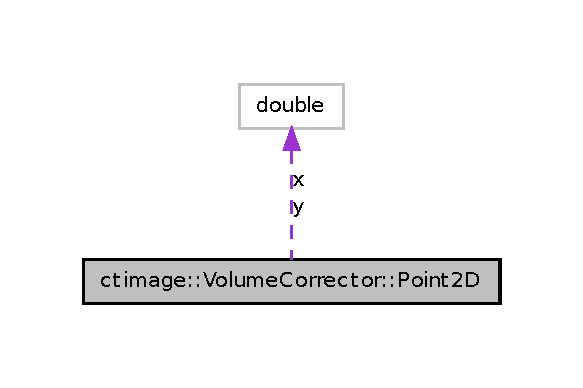
\includegraphics[width=280pt]{structctimage_1_1_volume_corrector_1_1_point2_d__coll__graph}
\end{center}
\end{figure}
\subsection*{Public Attributes}
\begin{DoxyCompactItemize}
\item 
\hypertarget{structctimage_1_1_volume_corrector_1_1_point2_d_a52e8a66faf11149515762ff083921ea3}{
double {\bfseries x}}
\label{structctimage_1_1_volume_corrector_1_1_point2_d_a52e8a66faf11149515762ff083921ea3}

\item 
\hypertarget{structctimage_1_1_volume_corrector_1_1_point2_d_ae95bae02c469e7dabe1d52b35e2d824a}{
double {\bfseries y}}
\label{structctimage_1_1_volume_corrector_1_1_point2_d_ae95bae02c469e7dabe1d52b35e2d824a}

\end{DoxyCompactItemize}


\subsection{Detailed Description}
A 2-\/Dimensional point. 

The documentation for this struct was generated from the following file:\begin{DoxyCompactItemize}
\item 
ctimage/VolumeCorrector.h\end{DoxyCompactItemize}

\hypertarget{classgui_1_1_assignment_actor}{
\section{gui::AssignmentActor Class Reference}
\label{classgui_1_1_assignment_actor}\index{gui::AssignmentActor@{gui::AssignmentActor}}
}


An \hyperlink{classvtk_prop_assembly}{vtkPropAssembly} containing an actor with a color map visualisation of a \hyperlink{classassignment_1_1_node_property_assigner}{assignment::NodePropertyAssigner} result and a vtkScalarBarActor with a corresponding color scale.  




{\ttfamily \#include $<$AssignmentActor.h$>$}



Inheritance diagram for gui::AssignmentActor:\nopagebreak
\begin{figure}[H]
\begin{center}
\leavevmode
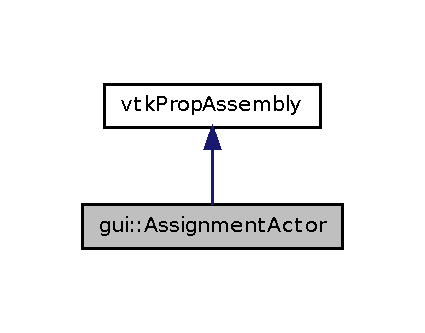
\includegraphics[width=204pt]{classgui_1_1_assignment_actor__inherit__graph}
\end{center}
\end{figure}


Collaboration diagram for gui::AssignmentActor:\nopagebreak
\begin{figure}[H]
\begin{center}
\leavevmode
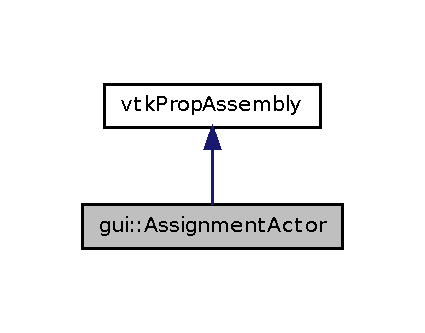
\includegraphics[width=204pt]{classgui_1_1_assignment_actor__coll__graph}
\end{center}
\end{figure}
\subsection*{Static Public Member Functions}
\begin{DoxyCompactItemize}
\item 
\hypertarget{classgui_1_1_assignment_actor_a550454472b7e6f8d4abc8470641e8090}{
static \hyperlink{classgui_1_1_assignment_actor}{AssignmentActor} $\ast$ \hyperlink{classgui_1_1_assignment_actor_a550454472b7e6f8d4abc8470641e8090}{New} (\hyperlink{classassignment_1_1_node_property_assigner}{assignment::NodePropertyAssigner} $\ast$)}
\label{classgui_1_1_assignment_actor_a550454472b7e6f8d4abc8470641e8090}

\begin{DoxyCompactList}\small\item\em Returns a new instance. \item\end{DoxyCompactList}\end{DoxyCompactItemize}


\subsection{Detailed Description}
An \hyperlink{classvtk_prop_assembly}{vtkPropAssembly} containing an actor with a color map visualisation of a \hyperlink{classassignment_1_1_node_property_assigner}{assignment::NodePropertyAssigner} result and a vtkScalarBarActor with a corresponding color scale. 

The documentation for this class was generated from the following files:\begin{DoxyCompactItemize}
\item 
gui/AssignmentActor.h\item 
gui/AssignmentActor.cxx\end{DoxyCompactItemize}

\hypertarget{classgui_1_1_main_window}{
\section{gui::MainWindow Class Reference}
\label{classgui_1_1_main_window}\index{gui::MainWindow@{gui::MainWindow}}
}


This class provides the main application window.  




{\ttfamily \#include $<$MainWindow.h$>$}



Inheritance diagram for gui::MainWindow:\nopagebreak
\begin{figure}[H]
\begin{center}
\leavevmode
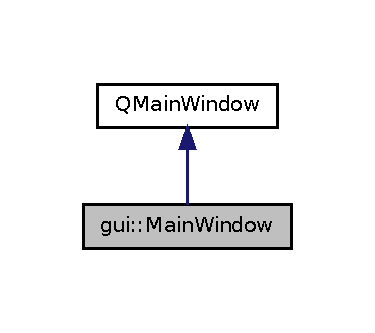
\includegraphics[width=180pt]{classgui_1_1_main_window__inherit__graph}
\end{center}
\end{figure}


Collaboration diagram for gui::MainWindow:\nopagebreak
\begin{figure}[H]
\begin{center}
\leavevmode
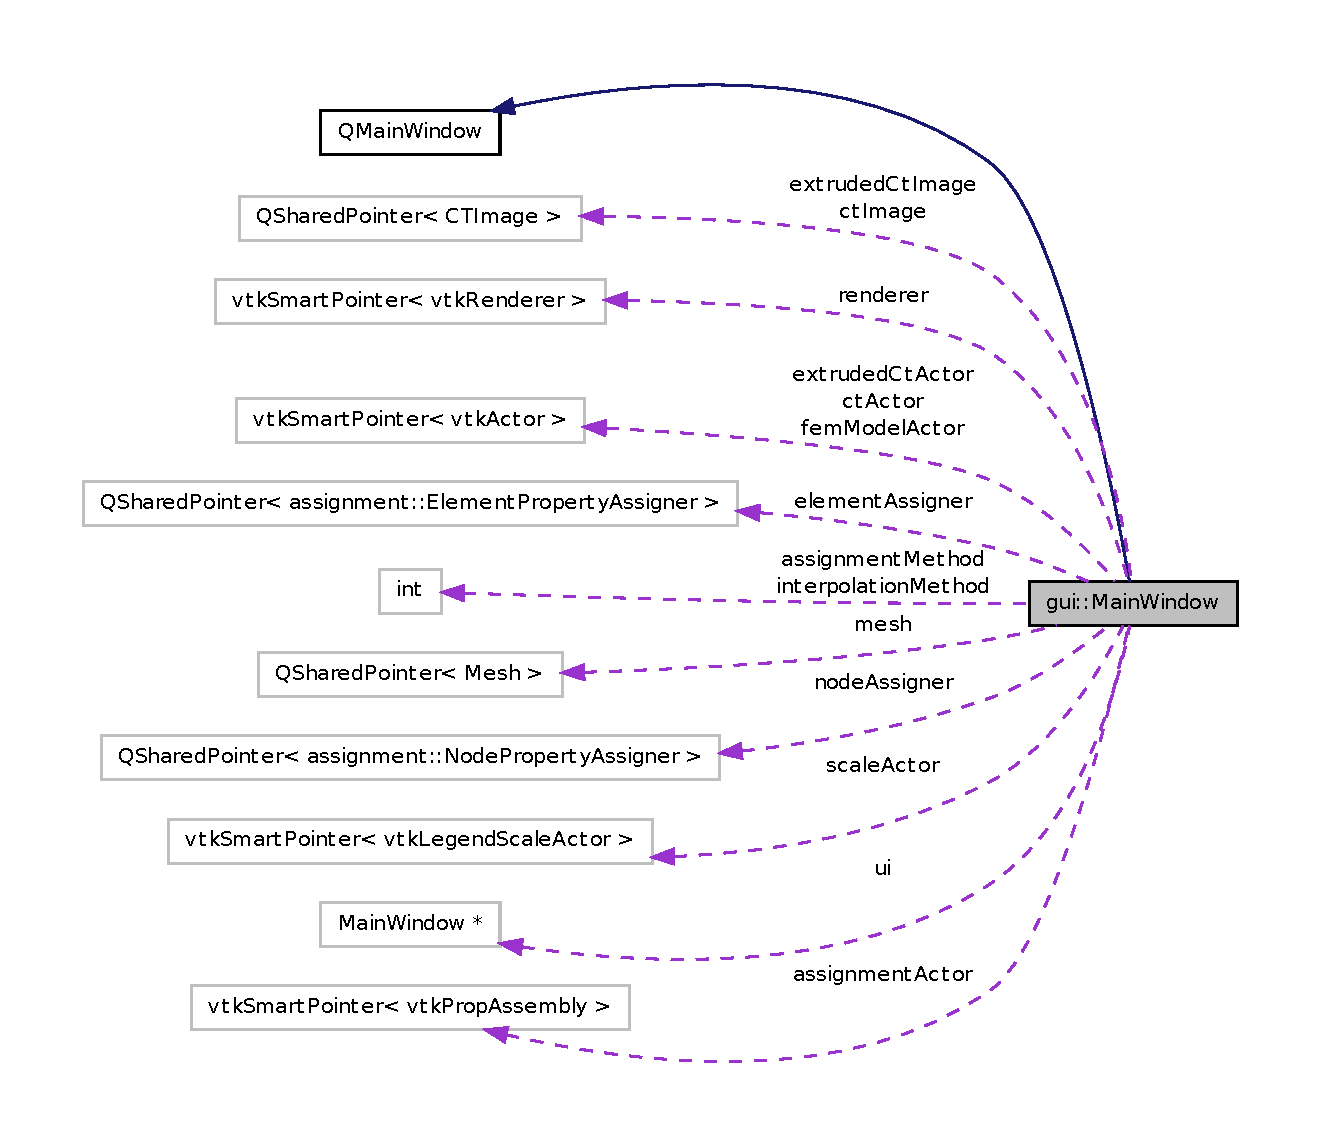
\includegraphics[width=400pt]{classgui_1_1_main_window__coll__graph}
\end{center}
\end{figure}
\subsection*{Public Member Functions}
\begin{DoxyCompactItemize}
\item 
\hyperlink{classgui_1_1_main_window_a712499e7b9b3c9d440d7b19a8865fc9f}{MainWindow} (QWidget $\ast$parent=0)
\begin{DoxyCompactList}\small\item\em Creates a new GUI window. \item\end{DoxyCompactList}\item 
\hypertarget{classgui_1_1_main_window_ab2de68292a3940a0f7956eb0e999ee04}{
void \hyperlink{classgui_1_1_main_window_ab2de68292a3940a0f7956eb0e999ee04}{showActor} (vtkSmartPointer$<$ vtkProp $>$, QCheckBox $\ast$)}
\label{classgui_1_1_main_window_ab2de68292a3940a0f7956eb0e999ee04}

\begin{DoxyCompactList}\small\item\em Displays a specified actor and enables/checks it's corresponding checkbox. \item\end{DoxyCompactList}\item 
\hypertarget{classgui_1_1_main_window_a5c68f604a32a0c8584be5a7590ad49c4}{
void \hyperlink{classgui_1_1_main_window_a5c68f604a32a0c8584be5a7590ad49c4}{hideActor} (vtkSmartPointer$<$ vtkProp $>$, QCheckBox $\ast$)}
\label{classgui_1_1_main_window_a5c68f604a32a0c8584be5a7590ad49c4}

\begin{DoxyCompactList}\small\item\em Hides a specified actor and disables/unchecks it's corresponding checkbox. \item\end{DoxyCompactList}\item 
\hypertarget{classgui_1_1_main_window_a4fd3872bcad0814f6e4bcc07fa9889bd}{
void \hyperlink{classgui_1_1_main_window_a4fd3872bcad0814f6e4bcc07fa9889bd}{clear} ()}
\label{classgui_1_1_main_window_a4fd3872bcad0814f6e4bcc07fa9889bd}

\begin{DoxyCompactList}\small\item\em Sets the window in its initial state. \item\end{DoxyCompactList}\end{DoxyCompactItemize}
\subsection*{Protected Member Functions}
\begin{DoxyCompactItemize}
\item 
\hypertarget{classgui_1_1_main_window_a62731a7857ecd07560e53a7b4cf0bd8b}{
void {\bfseries changeEvent} (QEvent $\ast$e)}
\label{classgui_1_1_main_window_a62731a7857ecd07560e53a7b4cf0bd8b}

\end{DoxyCompactItemize}
\subsection*{Private Slots}
\begin{DoxyCompactItemize}
\item 
void \hyperlink{classgui_1_1_main_window_ab6bc66d6d29c8ce9c25e42d23ca5796d}{toggleFEMModel} (int state)
\begin{DoxyCompactList}\small\item\em FEM model checkbox slot. \item\end{DoxyCompactList}\item 
void \hyperlink{classgui_1_1_main_window_a55e08f5a8915bb4838bdbd31b2bdaf4c}{toggleCTImage} (int state)
\begin{DoxyCompactList}\small\item\em CT image checkbox slot. \item\end{DoxyCompactList}\item 
void \hyperlink{classgui_1_1_main_window_a5102f72743b8fd8f6989eb339067e73f}{toggleExtrudedCTImage} (int state)
\begin{DoxyCompactList}\small\item\em Extruded CT image checkbox slot. \item\end{DoxyCompactList}\item 
void \hyperlink{classgui_1_1_main_window_ac3f9bab09dfb3646b0ee1be0bd613f20}{toggleAssignment} (int state)
\begin{DoxyCompactList}\small\item\em Assignment result checkbox slot. \item\end{DoxyCompactList}\item 
void \hyperlink{classgui_1_1_main_window_a4646ba0d34c86dfe969b285b00c30d5e}{toggleScale} (int state)
\begin{DoxyCompactList}\small\item\em Scale checkbox slot. \item\end{DoxyCompactList}\item 
void \hyperlink{classgui_1_1_main_window_a9d49a35ea4419d69f2f89950a8ffbdda}{toggleInterpolationMethod} (bool t)
\begin{DoxyCompactList}\small\item\em Interpolation method switch slot. \item\end{DoxyCompactList}\item 
void \hyperlink{classgui_1_1_main_window_a3891bbf7215a4c190a6c5392dadb0a29}{toggleAssignmentMethod} (bool t)
\begin{DoxyCompactList}\small\item\em Assignment method switch slot. \item\end{DoxyCompactList}\item 
\hypertarget{classgui_1_1_main_window_ab527d189efca4163ee27ae1ffbf12f94}{
void \hyperlink{classgui_1_1_main_window_ab527d189efca4163ee27ae1ffbf12f94}{loadAnsys} ()}
\label{classgui_1_1_main_window_ab527d189efca4163ee27ae1ffbf12f94}

\begin{DoxyCompactList}\small\item\em Ansys load button slot. \item\end{DoxyCompactList}\item 
\hypertarget{classgui_1_1_main_window_ab146d4d7203ae93b9a50b9a1f0613b55}{
void \hyperlink{classgui_1_1_main_window_ab146d4d7203ae93b9a50b9a1f0613b55}{loadAbaqus} ()}
\label{classgui_1_1_main_window_ab146d4d7203ae93b9a50b9a1f0613b55}

\begin{DoxyCompactList}\small\item\em Abaqus load button slot. \item\end{DoxyCompactList}\item 
\hypertarget{classgui_1_1_main_window_a256bb2202375fc3309ae5543dc8ffc8f}{
void \hyperlink{classgui_1_1_main_window_a256bb2202375fc3309ae5543dc8ffc8f}{loadDicom} ()}
\label{classgui_1_1_main_window_a256bb2202375fc3309ae5543dc8ffc8f}

\begin{DoxyCompactList}\small\item\em Dicom load button slot. \item\end{DoxyCompactList}\item 
\hypertarget{classgui_1_1_main_window_a0ae17d7d51bd4549b37a6d07165203ca}{
void \hyperlink{classgui_1_1_main_window_a0ae17d7d51bd4549b37a6d07165203ca}{loadMetafile} ()}
\label{classgui_1_1_main_window_a0ae17d7d51bd4549b37a6d07165203ca}

\begin{DoxyCompactList}\small\item\em Metaimage load button slot. \item\end{DoxyCompactList}\item 
void \hyperlink{classgui_1_1_main_window_ab8feef1bc2150a62f309cac1fc98b1f2}{extrusionSliderChanged} (int value)
\begin{DoxyCompactList}\small\item\em Extrusion slider slot. \item\end{DoxyCompactList}\item 
\hypertarget{classgui_1_1_main_window_a972f3a47296041eb91d74163e5940ac3}{
void \hyperlink{classgui_1_1_main_window_a972f3a47296041eb91d74163e5940ac3}{exportExtrudedImage} ()}
\label{classgui_1_1_main_window_a972f3a47296041eb91d74163e5940ac3}

\begin{DoxyCompactList}\small\item\em Dicom export slot. \item\end{DoxyCompactList}\item 
\hypertarget{classgui_1_1_main_window_a9ac823ee2e8cc81201e3601b8478c92c}{
void \hyperlink{classgui_1_1_main_window_a9ac823ee2e8cc81201e3601b8478c92c}{exportAnsys} ()}
\label{classgui_1_1_main_window_a9ac823ee2e8cc81201e3601b8478c92c}

\begin{DoxyCompactList}\small\item\em Ansys export slot. \item\end{DoxyCompactList}\item 
\hypertarget{classgui_1_1_main_window_a174e0d0ab437a2408b385b35798dd659}{
void \hyperlink{classgui_1_1_main_window_a174e0d0ab437a2408b385b35798dd659}{exportAbaqus} ()}
\label{classgui_1_1_main_window_a174e0d0ab437a2408b385b35798dd659}

\begin{DoxyCompactList}\small\item\em Abaqus export slot. \item\end{DoxyCompactList}\item 
\hypertarget{classgui_1_1_main_window_ab0fc116fbb9cb1df7c2f7dfd019402ab}{
void \hyperlink{classgui_1_1_main_window_ab0fc116fbb9cb1df7c2f7dfd019402ab}{run} ()}
\label{classgui_1_1_main_window_ab0fc116fbb9cb1df7c2f7dfd019402ab}

\begin{DoxyCompactList}\small\item\em Run button slot. \item\end{DoxyCompactList}\end{DoxyCompactItemize}
\subsection*{Private Member Functions}
\begin{DoxyCompactItemize}
\item 
\hypertarget{classgui_1_1_main_window_a9b53ad68c9a10d546ce4b4d171413e99}{
void \hyperlink{classgui_1_1_main_window_a9b53ad68c9a10d546ce4b4d171413e99}{loadMesh} ()}
\label{classgui_1_1_main_window_a9b53ad68c9a10d546ce4b4d171413e99}

\begin{DoxyCompactList}\small\item\em Loads the mesh into the GUI. \item\end{DoxyCompactList}\item 
\hypertarget{classgui_1_1_main_window_afbfceb6a660dff0cc5938e1783df41b4}{
void \hyperlink{classgui_1_1_main_window_afbfceb6a660dff0cc5938e1783df41b4}{loadCtImage} ()}
\label{classgui_1_1_main_window_afbfceb6a660dff0cc5938e1783df41b4}

\begin{DoxyCompactList}\small\item\em Loads the CT image into the GUI. \item\end{DoxyCompactList}\item 
void \hyperlink{classgui_1_1_main_window_ad47a9433cd59b71e66643004d182907d}{showMessage} (std::string msg)
\begin{DoxyCompactList}\small\item\em Displays a message to the user. \item\end{DoxyCompactList}\item 
bool \hyperlink{classgui_1_1_main_window_a85d3a7d16217e99e0fedcf0c65107f99}{checkLoadComplete} ()
\begin{DoxyCompactList}\small\item\em Checks if both the \hyperlink{classmesh_1_1_mesh}{mesh::Mesh} and \hyperlink{classctimage_1_1_c_t_image}{ctimage::CTImage} are loaded. \item\end{DoxyCompactList}\end{DoxyCompactItemize}
\subsection*{Private Attributes}
\begin{DoxyCompactItemize}
\item 
\hypertarget{classgui_1_1_main_window_a8fc767f398e4bebf05af19574db9fb0e}{
vtkSmartPointer$<$ vtkRenderer $>$ \hyperlink{classgui_1_1_main_window_a8fc767f398e4bebf05af19574db9fb0e}{renderer}}
\label{classgui_1_1_main_window_a8fc767f398e4bebf05af19574db9fb0e}

\begin{DoxyCompactList}\small\item\em The renderer. \item\end{DoxyCompactList}\item 
\hypertarget{classgui_1_1_main_window_a2e5976958b9de74939664b970a1c6be1}{
vtkSmartPointer$<$ vtkActor $>$ \hyperlink{classgui_1_1_main_window_a2e5976958b9de74939664b970a1c6be1}{femModelActor}}
\label{classgui_1_1_main_window_a2e5976958b9de74939664b970a1c6be1}

\begin{DoxyCompactList}\small\item\em The FEM model (mesh) actor. \item\end{DoxyCompactList}\item 
\hypertarget{classgui_1_1_main_window_a49c55c30152f0eb436de815d2ab65c4d}{
vtkSmartPointer$<$ vtkActor $>$ \hyperlink{classgui_1_1_main_window_a49c55c30152f0eb436de815d2ab65c4d}{ctActor}}
\label{classgui_1_1_main_window_a49c55c30152f0eb436de815d2ab65c4d}

\begin{DoxyCompactList}\small\item\em The CT image model / isosurface actor. \item\end{DoxyCompactList}\item 
\hypertarget{classgui_1_1_main_window_aaa081fb46c3e494dbdba6f15b1a54095}{
vtkSmartPointer$<$ vtkActor $>$ \hyperlink{classgui_1_1_main_window_aaa081fb46c3e494dbdba6f15b1a54095}{extrudedCtActor}}
\label{classgui_1_1_main_window_aaa081fb46c3e494dbdba6f15b1a54095}

\begin{DoxyCompactList}\small\item\em The extruded CT image model / isosurface actor. \item\end{DoxyCompactList}\item 
\hypertarget{classgui_1_1_main_window_a55e9ef04df1730c3c614f6ed1ed648de}{
vtkSmartPointer$<$ \hyperlink{classvtk_prop_assembly}{vtkPropAssembly} $>$ \hyperlink{classgui_1_1_main_window_a55e9ef04df1730c3c614f6ed1ed648de}{assignmentActor}}
\label{classgui_1_1_main_window_a55e9ef04df1730c3c614f6ed1ed648de}

\begin{DoxyCompactList}\small\item\em The assignment result actor. \item\end{DoxyCompactList}\item 
\hypertarget{classgui_1_1_main_window_a6dcbdf1bcf22df87077fa31aedc2da15}{
vtkSmartPointer$<$ vtkLegendScaleActor $>$ \hyperlink{classgui_1_1_main_window_a6dcbdf1bcf22df87077fa31aedc2da15}{scaleActor}}
\label{classgui_1_1_main_window_a6dcbdf1bcf22df87077fa31aedc2da15}

\begin{DoxyCompactList}\small\item\em The scale actor. \item\end{DoxyCompactList}\item 
\hypertarget{classgui_1_1_main_window_a8682deb203079f8f3f5d5df705e60703}{
Ui::MainWindow $\ast$ \hyperlink{classgui_1_1_main_window_a8682deb203079f8f3f5d5df705e60703}{ui}}
\label{classgui_1_1_main_window_a8682deb203079f8f3f5d5df705e60703}

\begin{DoxyCompactList}\small\item\em The QT form interface. \item\end{DoxyCompactList}\item 
\hypertarget{classgui_1_1_main_window_a3c687d09e6ac3432b3660bf6c0c1783f}{
QSharedPointer$<$ \hyperlink{classmesh_1_1_mesh}{Mesh} $>$ \hyperlink{classgui_1_1_main_window_a3c687d09e6ac3432b3660bf6c0c1783f}{mesh}}
\label{classgui_1_1_main_window_a3c687d09e6ac3432b3660bf6c0c1783f}

\begin{DoxyCompactList}\small\item\em The loaded \hyperlink{classmesh_1_1_mesh}{mesh::Mesh}. \item\end{DoxyCompactList}\item 
\hypertarget{classgui_1_1_main_window_ad25359ec4b7f6d23d292c3cf5d3e3e36}{
QSharedPointer$<$ \hyperlink{classctimage_1_1_c_t_image}{CTImage} $>$ \hyperlink{classgui_1_1_main_window_ad25359ec4b7f6d23d292c3cf5d3e3e36}{ctImage}}
\label{classgui_1_1_main_window_ad25359ec4b7f6d23d292c3cf5d3e3e36}

\begin{DoxyCompactList}\small\item\em The loaded \hyperlink{classctimage_1_1_c_t_image}{ctimage::CTImage}. \item\end{DoxyCompactList}\item 
\hypertarget{classgui_1_1_main_window_a301d15abf322ace147c5d6f20093830c}{
QSharedPointer$<$ \hyperlink{classctimage_1_1_c_t_image}{CTImage} $>$ \hyperlink{classgui_1_1_main_window_a301d15abf322ace147c5d6f20093830c}{extrudedCtImage}}
\label{classgui_1_1_main_window_a301d15abf322ace147c5d6f20093830c}

\begin{DoxyCompactList}\small\item\em The extruded \hyperlink{classctimage_1_1_c_t_image}{ctimage::CTImage}. \item\end{DoxyCompactList}\item 
\hypertarget{classgui_1_1_main_window_aebdf130c1f7a497215c52bad94d71975}{
int \hyperlink{classgui_1_1_main_window_aebdf130c1f7a497215c52bad94d71975}{interpolationMethod}}
\label{classgui_1_1_main_window_aebdf130c1f7a497215c52bad94d71975}

\begin{DoxyCompactList}\small\item\em The interpolation method. \item\end{DoxyCompactList}\item 
\hypertarget{classgui_1_1_main_window_ab4cab84ee3d3b9318a129ba7f456837c}{
int \hyperlink{classgui_1_1_main_window_ab4cab84ee3d3b9318a129ba7f456837c}{assignmentMethod}}
\label{classgui_1_1_main_window_ab4cab84ee3d3b9318a129ba7f456837c}

\begin{DoxyCompactList}\small\item\em The assignment method. \item\end{DoxyCompactList}\item 
\hypertarget{classgui_1_1_main_window_ad1fbd0a0da67c0e8f3378ee0415dfaa1}{
QSharedPointer$<$ \hyperlink{classassignment_1_1_node_property_assigner}{assignment::NodePropertyAssigner} $>$ \hyperlink{classgui_1_1_main_window_ad1fbd0a0da67c0e8f3378ee0415dfaa1}{nodeAssigner}}
\label{classgui_1_1_main_window_ad1fbd0a0da67c0e8f3378ee0415dfaa1}

\begin{DoxyCompactList}\small\item\em The node assigner. \item\end{DoxyCompactList}\item 
\hypertarget{classgui_1_1_main_window_a2f296c603ff5f915b6023370fb87acfd}{
QSharedPointer$<$ \hyperlink{classassignment_1_1_element_property_assigner}{assignment::ElementPropertyAssigner} $>$ \hyperlink{classgui_1_1_main_window_a2f296c603ff5f915b6023370fb87acfd}{elementAssigner}}
\label{classgui_1_1_main_window_a2f296c603ff5f915b6023370fb87acfd}

\begin{DoxyCompactList}\small\item\em The element assigner. \item\end{DoxyCompactList}\end{DoxyCompactItemize}


\subsection{Detailed Description}
This class provides the main application window. 

\subsection{Constructor \& Destructor Documentation}
\hypertarget{classgui_1_1_main_window_a712499e7b9b3c9d440d7b19a8865fc9f}{
\index{gui::MainWindow@{gui::MainWindow}!MainWindow@{MainWindow}}
\index{MainWindow@{MainWindow}!gui::MainWindow@{gui::MainWindow}}
\subsubsection[{MainWindow}]{\setlength{\rightskip}{0pt plus 5cm}gui::MainWindow::MainWindow (
\begin{DoxyParamCaption}
\item[{QWidget $\ast$}]{ parent = {\ttfamily 0}}
\end{DoxyParamCaption}
)}}
\label{classgui_1_1_main_window_a712499e7b9b3c9d440d7b19a8865fc9f}


Creates a new GUI window. 

\begin{DoxyNote}{Note}
The form is loaded from the QT form file mainwindow.ui 
\end{DoxyNote}


\subsection{Member Function Documentation}
\hypertarget{classgui_1_1_main_window_a85d3a7d16217e99e0fedcf0c65107f99}{
\index{gui::MainWindow@{gui::MainWindow}!checkLoadComplete@{checkLoadComplete}}
\index{checkLoadComplete@{checkLoadComplete}!gui::MainWindow@{gui::MainWindow}}
\subsubsection[{checkLoadComplete}]{\setlength{\rightskip}{0pt plus 5cm}bool gui::MainWindow::checkLoadComplete (
\begin{DoxyParamCaption}
{}
\end{DoxyParamCaption}
)\hspace{0.3cm}{\ttfamily  \mbox{[}private\mbox{]}}}}
\label{classgui_1_1_main_window_a85d3a7d16217e99e0fedcf0c65107f99}


Checks if both the \hyperlink{classmesh_1_1_mesh}{mesh::Mesh} and \hyperlink{classctimage_1_1_c_t_image}{ctimage::CTImage} are loaded. 

\begin{DoxyReturn}{Returns}
True if both the \hyperlink{classmesh_1_1_mesh}{mesh::Mesh} and \hyperlink{classctimage_1_1_c_t_image}{ctimage::CTImage} are loaded 
\end{DoxyReturn}
\hypertarget{classgui_1_1_main_window_ab8feef1bc2150a62f309cac1fc98b1f2}{
\index{gui::MainWindow@{gui::MainWindow}!extrusionSliderChanged@{extrusionSliderChanged}}
\index{extrusionSliderChanged@{extrusionSliderChanged}!gui::MainWindow@{gui::MainWindow}}
\subsubsection[{extrusionSliderChanged}]{\setlength{\rightskip}{0pt plus 5cm}void gui::MainWindow::extrusionSliderChanged (
\begin{DoxyParamCaption}
\item[{int}]{ value}
\end{DoxyParamCaption}
)\hspace{0.3cm}{\ttfamily  \mbox{[}private, slot\mbox{]}}}}
\label{classgui_1_1_main_window_ab8feef1bc2150a62f309cac1fc98b1f2}


Extrusion slider slot. 


\begin{DoxyParams}{Parameters}
\item[{\em The}]slider's value \end{DoxyParams}
\hypertarget{classgui_1_1_main_window_ad47a9433cd59b71e66643004d182907d}{
\index{gui::MainWindow@{gui::MainWindow}!showMessage@{showMessage}}
\index{showMessage@{showMessage}!gui::MainWindow@{gui::MainWindow}}
\subsubsection[{showMessage}]{\setlength{\rightskip}{0pt plus 5cm}void gui::MainWindow::showMessage (
\begin{DoxyParamCaption}
\item[{std::string}]{ msg}
\end{DoxyParamCaption}
)\hspace{0.3cm}{\ttfamily  \mbox{[}private\mbox{]}}}}
\label{classgui_1_1_main_window_ad47a9433cd59b71e66643004d182907d}


Displays a message to the user. 


\begin{DoxyParams}{Parameters}
\item[{\em The}]message to be displayed \end{DoxyParams}
\hypertarget{classgui_1_1_main_window_ac3f9bab09dfb3646b0ee1be0bd613f20}{
\index{gui::MainWindow@{gui::MainWindow}!toggleAssignment@{toggleAssignment}}
\index{toggleAssignment@{toggleAssignment}!gui::MainWindow@{gui::MainWindow}}
\subsubsection[{toggleAssignment}]{\setlength{\rightskip}{0pt plus 5cm}void gui::MainWindow::toggleAssignment (
\begin{DoxyParamCaption}
\item[{int}]{ state}
\end{DoxyParamCaption}
)\hspace{0.3cm}{\ttfamily  \mbox{[}private, slot\mbox{]}}}}
\label{classgui_1_1_main_window_ac3f9bab09dfb3646b0ee1be0bd613f20}


Assignment result checkbox slot. 


\begin{DoxyParams}{Parameters}
\item[{\em state}]Qt::Checked if the checkbox is in checked state \end{DoxyParams}
\hypertarget{classgui_1_1_main_window_a3891bbf7215a4c190a6c5392dadb0a29}{
\index{gui::MainWindow@{gui::MainWindow}!toggleAssignmentMethod@{toggleAssignmentMethod}}
\index{toggleAssignmentMethod@{toggleAssignmentMethod}!gui::MainWindow@{gui::MainWindow}}
\subsubsection[{toggleAssignmentMethod}]{\setlength{\rightskip}{0pt plus 5cm}void gui::MainWindow::toggleAssignmentMethod (
\begin{DoxyParamCaption}
\item[{bool}]{ t}
\end{DoxyParamCaption}
)\hspace{0.3cm}{\ttfamily  \mbox{[}private, slot\mbox{]}}}}
\label{classgui_1_1_main_window_a3891bbf7215a4c190a6c5392dadb0a29}


Assignment method switch slot. 


\begin{DoxyParams}{Parameters}
\item[{\em t}]\end{DoxyParams}
\hypertarget{classgui_1_1_main_window_a55e08f5a8915bb4838bdbd31b2bdaf4c}{
\index{gui::MainWindow@{gui::MainWindow}!toggleCTImage@{toggleCTImage}}
\index{toggleCTImage@{toggleCTImage}!gui::MainWindow@{gui::MainWindow}}
\subsubsection[{toggleCTImage}]{\setlength{\rightskip}{0pt plus 5cm}void gui::MainWindow::toggleCTImage (
\begin{DoxyParamCaption}
\item[{int}]{ state}
\end{DoxyParamCaption}
)\hspace{0.3cm}{\ttfamily  \mbox{[}private, slot\mbox{]}}}}
\label{classgui_1_1_main_window_a55e08f5a8915bb4838bdbd31b2bdaf4c}


CT image checkbox slot. 


\begin{DoxyParams}{Parameters}
\item[{\em state}]Qt::Checked if the checkbox is in checked state \end{DoxyParams}
\hypertarget{classgui_1_1_main_window_a5102f72743b8fd8f6989eb339067e73f}{
\index{gui::MainWindow@{gui::MainWindow}!toggleExtrudedCTImage@{toggleExtrudedCTImage}}
\index{toggleExtrudedCTImage@{toggleExtrudedCTImage}!gui::MainWindow@{gui::MainWindow}}
\subsubsection[{toggleExtrudedCTImage}]{\setlength{\rightskip}{0pt plus 5cm}void gui::MainWindow::toggleExtrudedCTImage (
\begin{DoxyParamCaption}
\item[{int}]{ state}
\end{DoxyParamCaption}
)\hspace{0.3cm}{\ttfamily  \mbox{[}private, slot\mbox{]}}}}
\label{classgui_1_1_main_window_a5102f72743b8fd8f6989eb339067e73f}


Extruded CT image checkbox slot. 


\begin{DoxyParams}{Parameters}
\item[{\em state}]Qt::Checked if the checkbox is in checked state \end{DoxyParams}
\hypertarget{classgui_1_1_main_window_ab6bc66d6d29c8ce9c25e42d23ca5796d}{
\index{gui::MainWindow@{gui::MainWindow}!toggleFEMModel@{toggleFEMModel}}
\index{toggleFEMModel@{toggleFEMModel}!gui::MainWindow@{gui::MainWindow}}
\subsubsection[{toggleFEMModel}]{\setlength{\rightskip}{0pt plus 5cm}void gui::MainWindow::toggleFEMModel (
\begin{DoxyParamCaption}
\item[{int}]{ state}
\end{DoxyParamCaption}
)\hspace{0.3cm}{\ttfamily  \mbox{[}private, slot\mbox{]}}}}
\label{classgui_1_1_main_window_ab6bc66d6d29c8ce9c25e42d23ca5796d}


FEM model checkbox slot. 


\begin{DoxyParams}{Parameters}
\item[{\em state}]Qt::Checked if the checkbox is in checked state \end{DoxyParams}
\hypertarget{classgui_1_1_main_window_a9d49a35ea4419d69f2f89950a8ffbdda}{
\index{gui::MainWindow@{gui::MainWindow}!toggleInterpolationMethod@{toggleInterpolationMethod}}
\index{toggleInterpolationMethod@{toggleInterpolationMethod}!gui::MainWindow@{gui::MainWindow}}
\subsubsection[{toggleInterpolationMethod}]{\setlength{\rightskip}{0pt plus 5cm}void gui::MainWindow::toggleInterpolationMethod (
\begin{DoxyParamCaption}
\item[{bool}]{ t}
\end{DoxyParamCaption}
)\hspace{0.3cm}{\ttfamily  \mbox{[}private, slot\mbox{]}}}}
\label{classgui_1_1_main_window_a9d49a35ea4419d69f2f89950a8ffbdda}


Interpolation method switch slot. 


\begin{DoxyParams}{Parameters}
\item[{\em t}]\end{DoxyParams}
\hypertarget{classgui_1_1_main_window_a4646ba0d34c86dfe969b285b00c30d5e}{
\index{gui::MainWindow@{gui::MainWindow}!toggleScale@{toggleScale}}
\index{toggleScale@{toggleScale}!gui::MainWindow@{gui::MainWindow}}
\subsubsection[{toggleScale}]{\setlength{\rightskip}{0pt plus 5cm}void gui::MainWindow::toggleScale (
\begin{DoxyParamCaption}
\item[{int}]{ state}
\end{DoxyParamCaption}
)\hspace{0.3cm}{\ttfamily  \mbox{[}private, slot\mbox{]}}}}
\label{classgui_1_1_main_window_a4646ba0d34c86dfe969b285b00c30d5e}


Scale checkbox slot. 


\begin{DoxyParams}{Parameters}
\item[{\em state}]Qt::Checked if the checkbox is in checked state \end{DoxyParams}


The documentation for this class was generated from the following files:\begin{DoxyCompactItemize}
\item 
gui/MainWindow.h\item 
gui/MainWindow.cxx\end{DoxyCompactItemize}

\hypertarget{classgui_1_1_vtk_poly_data_creator}{
\section{gui::VtkPolyDataCreator Class Reference}
\label{classgui_1_1_vtk_poly_data_creator}\index{gui::VtkPolyDataCreator@{gui::VtkPolyDataCreator}}
}


Creates the vtkPolyData object for a \hyperlink{classmesh_1_1_mesh}{mesh::Mesh}.  




{\ttfamily \#include $<$VtkPolyDataCreator.h$>$}

\subsection*{Static Public Member Functions}
\begin{DoxyCompactItemize}
\item 
static vtkSmartPointer$<$ vtkPolyData $>$ \hyperlink{classgui_1_1_vtk_poly_data_creator_aeaa631b114fc05c61c6a602fdbf0b3d9}{getVtkPolyData} (QSharedPointer$<$ \hyperlink{classmesh_1_1_mesh}{mesh::Mesh} $>$ mesh)
\begin{DoxyCompactList}\small\item\em Creates a new vtkPolyData object. \item\end{DoxyCompactList}\end{DoxyCompactItemize}


\subsection{Detailed Description}
Creates the vtkPolyData object for a \hyperlink{classmesh_1_1_mesh}{mesh::Mesh}. 

\subsection{Member Function Documentation}
\hypertarget{classgui_1_1_vtk_poly_data_creator_aeaa631b114fc05c61c6a602fdbf0b3d9}{
\index{gui::VtkPolyDataCreator@{gui::VtkPolyDataCreator}!getVtkPolyData@{getVtkPolyData}}
\index{getVtkPolyData@{getVtkPolyData}!gui::VtkPolyDataCreator@{gui::VtkPolyDataCreator}}
\subsubsection[{getVtkPolyData}]{\setlength{\rightskip}{0pt plus 5cm}vtkSmartPointer$<$ vtkPolyData $>$ gui::VtkPolyDataCreator::getVtkPolyData (
\begin{DoxyParamCaption}
\item[{QSharedPointer$<$ {\bf mesh::Mesh} $>$}]{ mesh}
\end{DoxyParamCaption}
)\hspace{0.3cm}{\ttfamily  \mbox{[}static\mbox{]}}}}
\label{classgui_1_1_vtk_poly_data_creator_aeaa631b114fc05c61c6a602fdbf0b3d9}


Creates a new vtkPolyData object. 


\begin{DoxyParams}{Parameters}
\item[{\em The}]\hyperlink{classmesh_1_1_mesh}{mesh::Mesh} the vtkPolyData is created from \end{DoxyParams}
\begin{DoxyReturn}{Returns}
A pointer to the created vtkPolyData object 
\end{DoxyReturn}


The documentation for this class was generated from the following files:\begin{DoxyCompactItemize}
\item 
gui/VtkPolyDataCreator.h\item 
gui/VtkPolyDataCreator.cxx\end{DoxyCompactItemize}

\hypertarget{classitk_1_1_image_to_v_t_k_image_filter}{
\section{itk::ImageToVTKImageFilter$<$ TInputImage $>$ Class Template Reference}
\label{classitk_1_1_image_to_v_t_k_image_filter}\index{itk::ImageToVTKImageFilter@{itk::ImageToVTKImageFilter}}
}


Converts an ITK image into a VTK image and plugs a itk data pipeline to a VTK datapipeline.  




{\ttfamily \#include $<$itkImageToVTKImageFilter.h$>$}



Inheritance diagram for itk::ImageToVTKImageFilter$<$ TInputImage $>$:\nopagebreak
\begin{figure}[H]
\begin{center}
\leavevmode
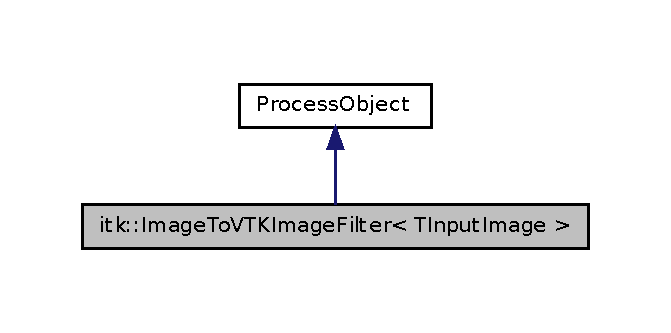
\includegraphics[width=322pt]{classitk_1_1_image_to_v_t_k_image_filter__inherit__graph}
\end{center}
\end{figure}


Collaboration diagram for itk::ImageToVTKImageFilter$<$ TInputImage $>$:\nopagebreak
\begin{figure}[H]
\begin{center}
\leavevmode
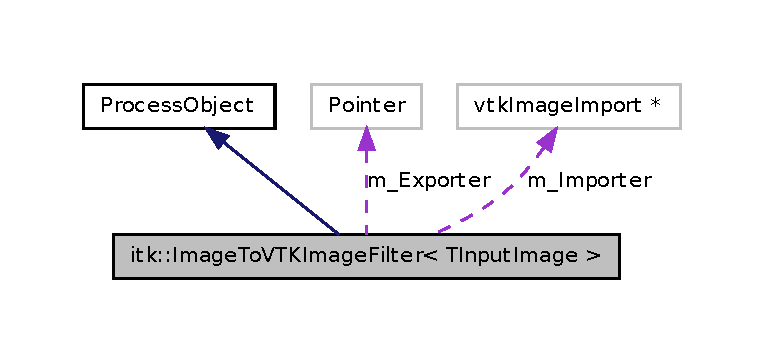
\includegraphics[width=366pt]{classitk_1_1_image_to_v_t_k_image_filter__coll__graph}
\end{center}
\end{figure}
\subsection*{Public Types}
\begin{DoxyCompactItemize}
\item 
typedef \hyperlink{classitk_1_1_image_to_v_t_k_image_filter}{ImageToVTKImageFilter} \hyperlink{classitk_1_1_image_to_v_t_k_image_filter_aa50164b556fb84d67e8631f5649d13e9}{Self}
\begin{DoxyCompactList}\small\item\em Standard class typedefs. \item\end{DoxyCompactList}\item 
\hypertarget{classitk_1_1_image_to_v_t_k_image_filter_a6fd526e20e86c11e356390cbf37191a8}{
typedef \hyperlink{class_process_object}{ProcessObject} {\bfseries Superclass}}
\label{classitk_1_1_image_to_v_t_k_image_filter_a6fd526e20e86c11e356390cbf37191a8}

\item 
\hypertarget{classitk_1_1_image_to_v_t_k_image_filter_a3400da105749199d5143f0e63bb0c768}{
typedef SmartPointer$<$ \hyperlink{classitk_1_1_image_to_v_t_k_image_filter}{Self} $>$ {\bfseries Pointer}}
\label{classitk_1_1_image_to_v_t_k_image_filter_a3400da105749199d5143f0e63bb0c768}

\item 
\hypertarget{classitk_1_1_image_to_v_t_k_image_filter_a058254c76c526a16dca79770886f0357}{
typedef SmartPointer$<$ const \hyperlink{classitk_1_1_image_to_v_t_k_image_filter}{Self} $>$ {\bfseries ConstPointer}}
\label{classitk_1_1_image_to_v_t_k_image_filter_a058254c76c526a16dca79770886f0357}

\item 
typedef TInputImage \hyperlink{classitk_1_1_image_to_v_t_k_image_filter_a4676ef1161730b61cddaf6ac892662f3}{InputImageType}
\begin{DoxyCompactList}\small\item\em Some typedefs. \item\end{DoxyCompactList}\item 
\hypertarget{classitk_1_1_image_to_v_t_k_image_filter_a3138f40f2bc46018bc6647e9f041fafe}{
typedef InputImageType::ConstPointer {\bfseries InputImagePointer}}
\label{classitk_1_1_image_to_v_t_k_image_filter_a3138f40f2bc46018bc6647e9f041fafe}

\item 
\hypertarget{classitk_1_1_image_to_v_t_k_image_filter_a03c5b387b58f71dbbbc5dfcbeaf0d05b}{
typedef VTKImageExport$<$ \hyperlink{classitk_1_1_image_to_v_t_k_image_filter_a4676ef1161730b61cddaf6ac892662f3}{InputImageType} $>$ {\bfseries ExporterFilterType}}
\label{classitk_1_1_image_to_v_t_k_image_filter_a03c5b387b58f71dbbbc5dfcbeaf0d05b}

\item 
\hypertarget{classitk_1_1_image_to_v_t_k_image_filter_a52a58193bdb8d61c70f0708770c1cbc6}{
typedef ExporterFilterType::Pointer {\bfseries ExporterFilterPointer}}
\label{classitk_1_1_image_to_v_t_k_image_filter_a52a58193bdb8d61c70f0708770c1cbc6}

\end{DoxyCompactItemize}
\subsection*{Public Member Functions}
\begin{DoxyCompactItemize}
\item 
\hyperlink{classitk_1_1_image_to_v_t_k_image_filter_aa710a87cb782de6debe331a86646f7b0}{itkNewMacro} (\hyperlink{classitk_1_1_image_to_v_t_k_image_filter}{Self})
\begin{DoxyCompactList}\small\item\em Method for creation through the object factory. \item\end{DoxyCompactList}\item 
\hyperlink{classitk_1_1_image_to_v_t_k_image_filter_a2660682c96fa14496eaff4226d9d6f38}{itkTypeMacro} (\hyperlink{classitk_1_1_image_to_v_t_k_image_filter}{ImageToVTKImageFilter}, \hyperlink{class_process_object}{ProcessObject})
\begin{DoxyCompactList}\small\item\em Run-\/time type information (and related methods). \item\end{DoxyCompactList}\item 
vtkImageData $\ast$ \hyperlink{classitk_1_1_image_to_v_t_k_image_filter_ac97a69a27292b89146503bac2182cd76}{GetOutput} () const 
\begin{DoxyCompactList}\small\item\em Get the output in the form of a vtkImage. \item\end{DoxyCompactList}\item 
\hypertarget{classitk_1_1_image_to_v_t_k_image_filter_a6cab58f7167a357889763a2412d6a9e5}{
void \hyperlink{classitk_1_1_image_to_v_t_k_image_filter_a6cab58f7167a357889763a2412d6a9e5}{SetInput} (const \hyperlink{classitk_1_1_image_to_v_t_k_image_filter_a4676ef1161730b61cddaf6ac892662f3}{InputImageType} $\ast$)}
\label{classitk_1_1_image_to_v_t_k_image_filter_a6cab58f7167a357889763a2412d6a9e5}

\begin{DoxyCompactList}\small\item\em Set the input in the form of an itk::Image. \item\end{DoxyCompactList}\item 
vtkImageImport $\ast$ \hyperlink{classitk_1_1_image_to_v_t_k_image_filter_ac7662c1a28f84be41a998348122aa1e6}{GetImporter} () const 
\begin{DoxyCompactList}\small\item\em Return the internal VTK image importer filter. \item\end{DoxyCompactList}\item 
ExporterFilterType $\ast$ \hyperlink{classitk_1_1_image_to_v_t_k_image_filter_a28148e706b46194ef4a812873e67f8b7}{GetExporter} () const 
\begin{DoxyCompactList}\small\item\em Return the internal ITK image exporter filter. \item\end{DoxyCompactList}\item 
\hypertarget{classitk_1_1_image_to_v_t_k_image_filter_ad852dddc5730024d756135faa6653158}{
void \hyperlink{classitk_1_1_image_to_v_t_k_image_filter_ad852dddc5730024d756135faa6653158}{Update} ()}
\label{classitk_1_1_image_to_v_t_k_image_filter_ad852dddc5730024d756135faa6653158}

\begin{DoxyCompactList}\small\item\em This call delegate the update to the importer. \item\end{DoxyCompactList}\end{DoxyCompactItemize}
\subsection*{Private Member Functions}
\begin{DoxyCompactItemize}
\item 
\hypertarget{classitk_1_1_image_to_v_t_k_image_filter_a9d02505a749f0e3a84ef3545d8e26d1b}{
{\bfseries ImageToVTKImageFilter} (const \hyperlink{classitk_1_1_image_to_v_t_k_image_filter}{Self} \&)}
\label{classitk_1_1_image_to_v_t_k_image_filter_a9d02505a749f0e3a84ef3545d8e26d1b}

\item 
\hypertarget{classitk_1_1_image_to_v_t_k_image_filter_a77dca048172100d69033d3c486009245}{
void {\bfseries operator=} (const \hyperlink{classitk_1_1_image_to_v_t_k_image_filter}{Self} \&)}
\label{classitk_1_1_image_to_v_t_k_image_filter_a77dca048172100d69033d3c486009245}

\end{DoxyCompactItemize}
\subsection*{Private Attributes}
\begin{DoxyCompactItemize}
\item 
\hypertarget{classitk_1_1_image_to_v_t_k_image_filter_ad00d5fde8d41cff1c67157a4db345d9d}{
ExporterFilterPointer {\bfseries m\_\-Exporter}}
\label{classitk_1_1_image_to_v_t_k_image_filter_ad00d5fde8d41cff1c67157a4db345d9d}

\item 
\hypertarget{classitk_1_1_image_to_v_t_k_image_filter_a767ad68d2686e62cee454d3776d6efe8}{
vtkImageImport $\ast$ {\bfseries m\_\-Importer}}
\label{classitk_1_1_image_to_v_t_k_image_filter_a767ad68d2686e62cee454d3776d6efe8}

\end{DoxyCompactItemize}


\subsection{Detailed Description}
\subsubsection*{template$<$class TInputImage$>$ class itk::ImageToVTKImageFilter$<$ TInputImage $>$}

Converts an ITK image into a VTK image and plugs a itk data pipeline to a VTK datapipeline. This class puts together an itkVTKImageExporter and a vtkImageImporter. It takes care of the details related to the connection of ITK and VTK pipelines. The User will perceive this filter as an adaptor to which an itk::Image can be plugged as input and a vtkImage is produced as output. 

\subsection{Member Typedef Documentation}
\hypertarget{classitk_1_1_image_to_v_t_k_image_filter_a4676ef1161730b61cddaf6ac892662f3}{
\index{itk::ImageToVTKImageFilter@{itk::ImageToVTKImageFilter}!InputImageType@{InputImageType}}
\index{InputImageType@{InputImageType}!itk::ImageToVTKImageFilter@{itk::ImageToVTKImageFilter}}
\subsubsection[{InputImageType}]{\setlength{\rightskip}{0pt plus 5cm}template$<$class TInputImage $>$ typedef TInputImage {\bf itk::ImageToVTKImageFilter}$<$ TInputImage $>$::{\bf InputImageType}}}
\label{classitk_1_1_image_to_v_t_k_image_filter_a4676ef1161730b61cddaf6ac892662f3}


Some typedefs. 

\hypertarget{classitk_1_1_image_to_v_t_k_image_filter_aa50164b556fb84d67e8631f5649d13e9}{
\index{itk::ImageToVTKImageFilter@{itk::ImageToVTKImageFilter}!Self@{Self}}
\index{Self@{Self}!itk::ImageToVTKImageFilter@{itk::ImageToVTKImageFilter}}
\subsubsection[{Self}]{\setlength{\rightskip}{0pt plus 5cm}template$<$class TInputImage $>$ typedef {\bf ImageToVTKImageFilter} {\bf itk::ImageToVTKImageFilter}$<$ TInputImage $>$::{\bf Self}}}
\label{classitk_1_1_image_to_v_t_k_image_filter_aa50164b556fb84d67e8631f5649d13e9}


Standard class typedefs. 



\subsection{Member Function Documentation}
\hypertarget{classitk_1_1_image_to_v_t_k_image_filter_a28148e706b46194ef4a812873e67f8b7}{
\index{itk::ImageToVTKImageFilter@{itk::ImageToVTKImageFilter}!GetExporter@{GetExporter}}
\index{GetExporter@{GetExporter}!itk::ImageToVTKImageFilter@{itk::ImageToVTKImageFilter}}
\subsubsection[{GetExporter}]{\setlength{\rightskip}{0pt plus 5cm}template$<$class TInputImage $>$ ExporterFilterType$\ast$ {\bf itk::ImageToVTKImageFilter}$<$ TInputImage $>$::GetExporter (
\begin{DoxyParamCaption}
{}
\end{DoxyParamCaption}
) const}}
\label{classitk_1_1_image_to_v_t_k_image_filter_a28148e706b46194ef4a812873e67f8b7}


Return the internal ITK image exporter filter. 

This is intended to facilitate users the access to methods in the exporter \hypertarget{classitk_1_1_image_to_v_t_k_image_filter_ac7662c1a28f84be41a998348122aa1e6}{
\index{itk::ImageToVTKImageFilter@{itk::ImageToVTKImageFilter}!GetImporter@{GetImporter}}
\index{GetImporter@{GetImporter}!itk::ImageToVTKImageFilter@{itk::ImageToVTKImageFilter}}
\subsubsection[{GetImporter}]{\setlength{\rightskip}{0pt plus 5cm}template$<$class TInputImage $>$ vtkImageImport$\ast$ {\bf itk::ImageToVTKImageFilter}$<$ TInputImage $>$::GetImporter (
\begin{DoxyParamCaption}
{}
\end{DoxyParamCaption}
) const}}
\label{classitk_1_1_image_to_v_t_k_image_filter_ac7662c1a28f84be41a998348122aa1e6}


Return the internal VTK image importer filter. 

This is intended to facilitate users the access to methods in the importer \hypertarget{classitk_1_1_image_to_v_t_k_image_filter_ac97a69a27292b89146503bac2182cd76}{
\index{itk::ImageToVTKImageFilter@{itk::ImageToVTKImageFilter}!GetOutput@{GetOutput}}
\index{GetOutput@{GetOutput}!itk::ImageToVTKImageFilter@{itk::ImageToVTKImageFilter}}
\subsubsection[{GetOutput}]{\setlength{\rightskip}{0pt plus 5cm}template$<$class TInputImage $>$ vtkImageData$\ast$ {\bf itk::ImageToVTKImageFilter}$<$ TInputImage $>$::GetOutput (
\begin{DoxyParamCaption}
{}
\end{DoxyParamCaption}
) const}}
\label{classitk_1_1_image_to_v_t_k_image_filter_ac97a69a27292b89146503bac2182cd76}


Get the output in the form of a vtkImage. 

This call is delegated to the internal vtkImageImporter filter \hypertarget{classitk_1_1_image_to_v_t_k_image_filter_aa710a87cb782de6debe331a86646f7b0}{
\index{itk::ImageToVTKImageFilter@{itk::ImageToVTKImageFilter}!itkNewMacro@{itkNewMacro}}
\index{itkNewMacro@{itkNewMacro}!itk::ImageToVTKImageFilter@{itk::ImageToVTKImageFilter}}
\subsubsection[{itkNewMacro}]{\setlength{\rightskip}{0pt plus 5cm}template$<$class TInputImage $>$ {\bf itk::ImageToVTKImageFilter}$<$ TInputImage $>$::itkNewMacro (
\begin{DoxyParamCaption}
\item[{{\bf Self}}]{}
\end{DoxyParamCaption}
)}}
\label{classitk_1_1_image_to_v_t_k_image_filter_aa710a87cb782de6debe331a86646f7b0}


Method for creation through the object factory. 

\hypertarget{classitk_1_1_image_to_v_t_k_image_filter_a2660682c96fa14496eaff4226d9d6f38}{
\index{itk::ImageToVTKImageFilter@{itk::ImageToVTKImageFilter}!itkTypeMacro@{itkTypeMacro}}
\index{itkTypeMacro@{itkTypeMacro}!itk::ImageToVTKImageFilter@{itk::ImageToVTKImageFilter}}
\subsubsection[{itkTypeMacro}]{\setlength{\rightskip}{0pt plus 5cm}template$<$class TInputImage $>$ {\bf itk::ImageToVTKImageFilter}$<$ TInputImage $>$::itkTypeMacro (
\begin{DoxyParamCaption}
\item[{{\bf ImageToVTKImageFilter}$<$ TInputImage $>$}]{, }
\item[{{\bf ProcessObject}}]{}
\end{DoxyParamCaption}
)}}
\label{classitk_1_1_image_to_v_t_k_image_filter_a2660682c96fa14496eaff4226d9d6f38}


Run-\/time type information (and related methods). 



The documentation for this class was generated from the following file:\begin{DoxyCompactItemize}
\item 
itkImageToVTKImageFilter.h\end{DoxyCompactItemize}

\hypertarget{class_logger}{
\section{Logger Class Reference}
\label{class_logger}\index{Logger@{Logger}}
}


Collaboration diagram for Logger:\nopagebreak
\begin{figure}[H]
\begin{center}
\leavevmode
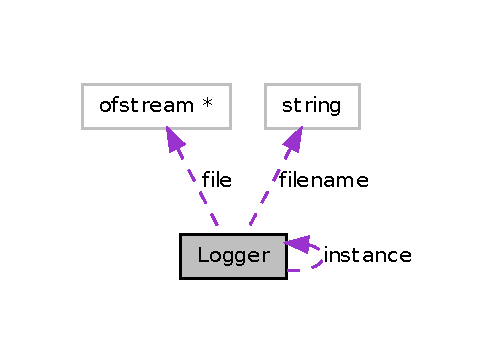
\includegraphics[width=239pt]{class_logger__coll__graph}
\end{center}
\end{figure}
\subsection*{Public Member Functions}
\begin{DoxyCompactItemize}
\item 
\hypertarget{class_logger_a01acea87f4fb7a014b78cb86d61b3601}{
{\footnotesize template$<$class T $>$ }\\void {\bfseries log} (T value)}
\label{class_logger_a01acea87f4fb7a014b78cb86d61b3601}

\item 
\hypertarget{class_logger_a53416a3009f942c74e37011b88dd58de}{
void {\bfseries log} (string)}
\label{class_logger_a53416a3009f942c74e37011b88dd58de}

\item 
\hypertarget{class_logger_a62b3477c22a38306a6d14ed7c134eade}{
void {\bfseries logError} (string)}
\label{class_logger_a62b3477c22a38306a6d14ed7c134eade}

\end{DoxyCompactItemize}
\subsection*{Static Public Member Functions}
\begin{DoxyCompactItemize}
\item 
\hypertarget{class_logger_afec28ae6d7bdf8f6a0734cb20756de10}{
static \hyperlink{class_logger}{Logger} $\ast$ {\bfseries getInstance} ()}
\label{class_logger_afec28ae6d7bdf8f6a0734cb20756de10}

\end{DoxyCompactItemize}
\subsection*{Private Member Functions}
\begin{DoxyCompactItemize}
\item 
\hypertarget{class_logger_a717fb11db9ded613d29b4618d60fc18a}{
{\bfseries Logger} (string)}
\label{class_logger_a717fb11db9ded613d29b4618d60fc18a}

\end{DoxyCompactItemize}
\subsection*{Private Attributes}
\begin{DoxyCompactItemize}
\item 
\hypertarget{class_logger_a6e5a0f90ab88e9c527a7847c6c929518}{
ofstream $\ast$ {\bfseries file}}
\label{class_logger_a6e5a0f90ab88e9c527a7847c6c929518}

\item 
\hypertarget{class_logger_abf648bfb3d3efd642ee175f00e2e8164}{
string {\bfseries filename}}
\label{class_logger_abf648bfb3d3efd642ee175f00e2e8164}

\end{DoxyCompactItemize}
\subsection*{Static Private Attributes}
\begin{DoxyCompactItemize}
\item 
\hypertarget{class_logger_a5e9fd267cd621afeb1201131071425ea}{
static \hyperlink{class_logger}{Logger} $\ast$ {\bfseries instance} = new \hyperlink{class_logger}{Logger}(\char`\"{}log.txt\char`\"{})}
\label{class_logger_a5e9fd267cd621afeb1201131071425ea}

\end{DoxyCompactItemize}


The documentation for this class was generated from the following files:\begin{DoxyCompactItemize}
\item 
Logger.h\item 
Logger.cxx\end{DoxyCompactItemize}

\hypertarget{classmesh_1_1_abaqus_element_property_writer}{
\section{mesh::AbaqusElementPropertyWriter Class Reference}
\label{classmesh_1_1_abaqus_element_property_writer}\index{mesh::AbaqusElementPropertyWriter@{mesh::AbaqusElementPropertyWriter}}
}


Writes a mesh file with element property assignment information to disk in Abaqus format.  




{\ttfamily \#include $<$AbaqusElementPropertyWriter.h$>$}



Inheritance diagram for mesh::AbaqusElementPropertyWriter:\nopagebreak
\begin{figure}[H]
\begin{center}
\leavevmode
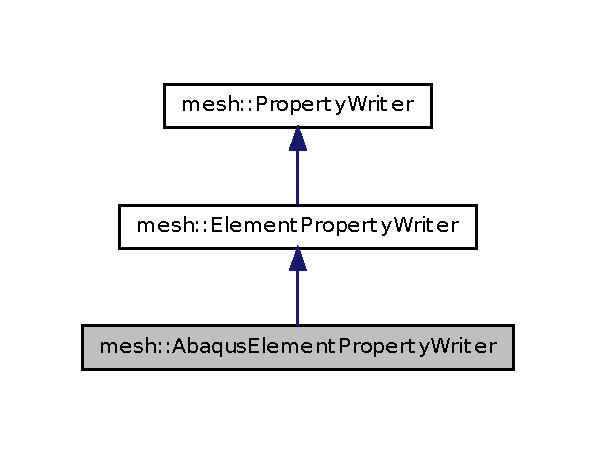
\includegraphics[width=286pt]{classmesh_1_1_abaqus_element_property_writer__inherit__graph}
\end{center}
\end{figure}


Collaboration diagram for mesh::AbaqusElementPropertyWriter:\nopagebreak
\begin{figure}[H]
\begin{center}
\leavevmode
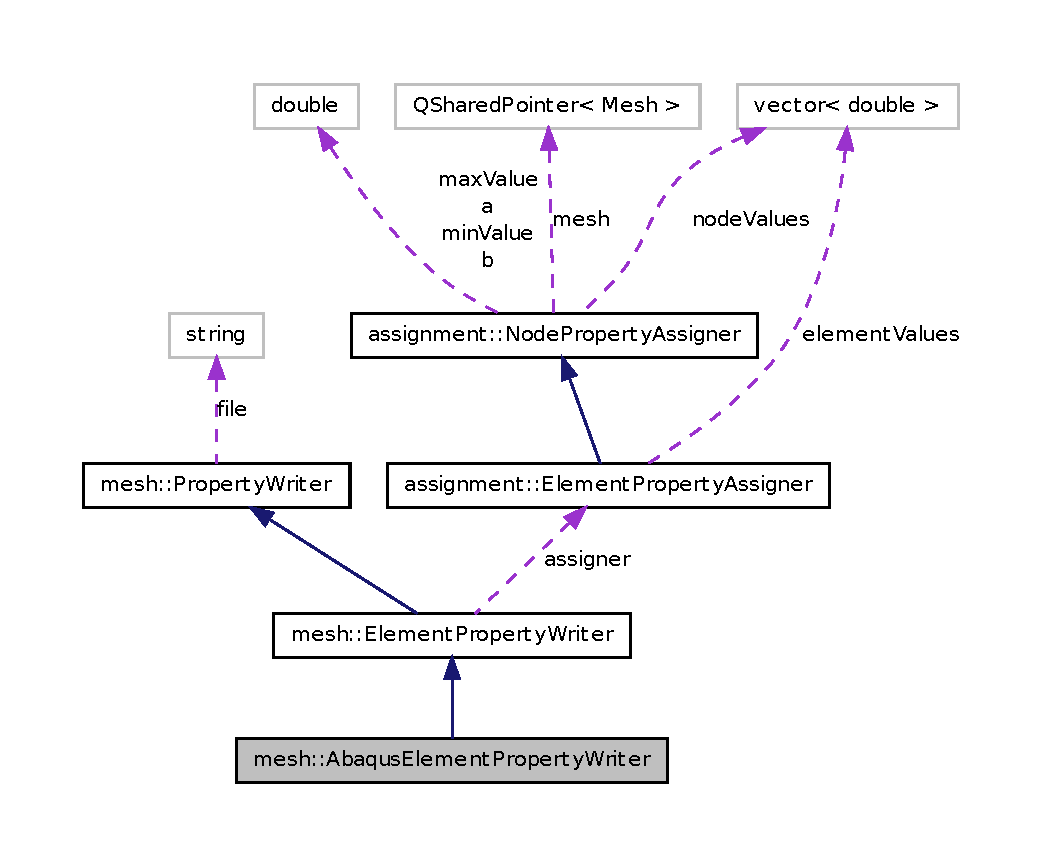
\includegraphics[width=400pt]{classmesh_1_1_abaqus_element_property_writer__coll__graph}
\end{center}
\end{figure}
\subsection*{Public Member Functions}
\begin{DoxyCompactItemize}
\item 
\hyperlink{classmesh_1_1_abaqus_element_property_writer_a1b6aa7b60c8a5810057aa64282d34d54}{AbaqusElementPropertyWriter} (string \hyperlink{classmesh_1_1_property_writer_a296638bd6daba8a6545688bacfc4fef1}{file}, \hyperlink{classassignment_1_1_element_property_assigner}{assignment::ElementPropertyAssigner} $\ast$\hyperlink{classmesh_1_1_element_property_writer_a2b64c6f7960645dd64fa9e1e62f2ac10}{assigner})
\begin{DoxyCompactList}\small\item\em Creates a new writer. \item\end{DoxyCompactList}\item 
\hypertarget{classmesh_1_1_abaqus_element_property_writer_aedd83e33ee64794cb616cc990ffceac7}{
void \hyperlink{classmesh_1_1_abaqus_element_property_writer_aedd83e33ee64794cb616cc990ffceac7}{write} ()}
\label{classmesh_1_1_abaqus_element_property_writer_aedd83e33ee64794cb616cc990ffceac7}

\begin{DoxyCompactList}\small\item\em Writes the file. \item\end{DoxyCompactList}\end{DoxyCompactItemize}


\subsection{Detailed Description}
Writes a mesh file with element property assignment information to disk in Abaqus format. 

\subsection{Constructor \& Destructor Documentation}
\hypertarget{classmesh_1_1_abaqus_element_property_writer_a1b6aa7b60c8a5810057aa64282d34d54}{
\index{mesh::AbaqusElementPropertyWriter@{mesh::AbaqusElementPropertyWriter}!AbaqusElementPropertyWriter@{AbaqusElementPropertyWriter}}
\index{AbaqusElementPropertyWriter@{AbaqusElementPropertyWriter}!mesh::AbaqusElementPropertyWriter@{mesh::AbaqusElementPropertyWriter}}
\subsubsection[{AbaqusElementPropertyWriter}]{\setlength{\rightskip}{0pt plus 5cm}mesh::AbaqusElementPropertyWriter::AbaqusElementPropertyWriter (
\begin{DoxyParamCaption}
\item[{string}]{ file, }
\item[{{\bf assignment::ElementPropertyAssigner} $\ast$}]{ assigner}
\end{DoxyParamCaption}
)}}
\label{classmesh_1_1_abaqus_element_property_writer_a1b6aa7b60c8a5810057aa64282d34d54}


Creates a new writer. 


\begin{DoxyParams}{Parameters}
\item[{\em file}]The file string \item[{\em assigner}]The \hyperlink{classassignment_1_1_element_property_assigner}{assignment::ElementPropertyAssigner} \end{DoxyParams}


The documentation for this class was generated from the following files:\begin{DoxyCompactItemize}
\item 
mesh/AbaqusElementPropertyWriter.h\item 
mesh/AbaqusElementPropertyWriter.cxx\end{DoxyCompactItemize}

\hypertarget{classmesh_1_1_abaqus_mesh_loader}{
\section{mesh::AbaqusMeshLoader Class Reference}
\label{classmesh_1_1_abaqus_mesh_loader}\index{mesh::AbaqusMeshLoader@{mesh::AbaqusMeshLoader}}
}


Loads an Abaqus mesh file from disk.  




{\ttfamily \#include $<$AbaqusMeshLoader.h$>$}



Inheritance diagram for mesh::AbaqusMeshLoader:\nopagebreak
\begin{figure}[H]
\begin{center}
\leavevmode
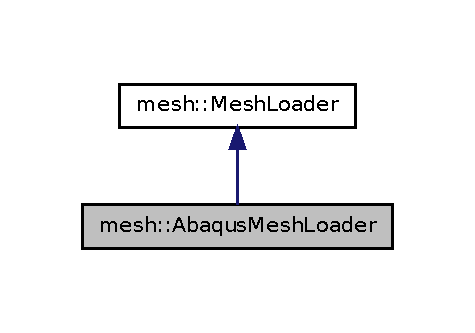
\includegraphics[width=228pt]{classmesh_1_1_abaqus_mesh_loader__inherit__graph}
\end{center}
\end{figure}


Collaboration diagram for mesh::AbaqusMeshLoader:\nopagebreak
\begin{figure}[H]
\begin{center}
\leavevmode
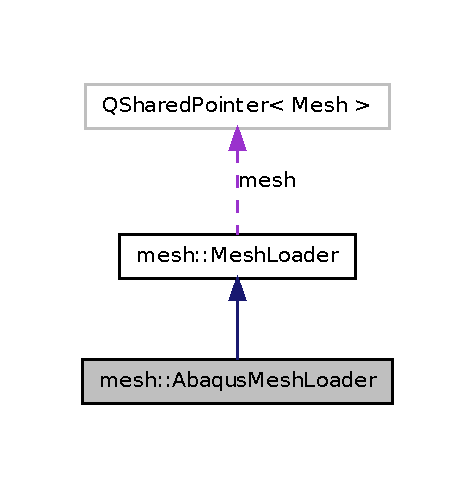
\includegraphics[width=228pt]{classmesh_1_1_abaqus_mesh_loader__coll__graph}
\end{center}
\end{figure}
\subsection*{Public Member Functions}
\begin{DoxyCompactItemize}
\item 
\hyperlink{classmesh_1_1_abaqus_mesh_loader_aca00ed54c0512c8c431a9ddc3fa77b7e}{AbaqusMeshLoader} (string file)
\begin{DoxyCompactList}\small\item\em Creates a new loader and reads the specified Abaqus file. \item\end{DoxyCompactList}\end{DoxyCompactItemize}
\subsection*{Private Member Functions}
\begin{DoxyCompactItemize}
\item 
\hypertarget{classmesh_1_1_abaqus_mesh_loader_a0799196c4a676dd0dc766b6cd9691b8d}{
void {\bfseries findSurfaceNodes} ()}
\label{classmesh_1_1_abaqus_mesh_loader_a0799196c4a676dd0dc766b6cd9691b8d}

\end{DoxyCompactItemize}


\subsection{Detailed Description}
Loads an Abaqus mesh file from disk. 

\subsection{Constructor \& Destructor Documentation}
\hypertarget{classmesh_1_1_abaqus_mesh_loader_aca00ed54c0512c8c431a9ddc3fa77b7e}{
\index{mesh::AbaqusMeshLoader@{mesh::AbaqusMeshLoader}!AbaqusMeshLoader@{AbaqusMeshLoader}}
\index{AbaqusMeshLoader@{AbaqusMeshLoader}!mesh::AbaqusMeshLoader@{mesh::AbaqusMeshLoader}}
\subsubsection[{AbaqusMeshLoader}]{\setlength{\rightskip}{0pt plus 5cm}mesh::AbaqusMeshLoader::AbaqusMeshLoader (
\begin{DoxyParamCaption}
\item[{string}]{ file}
\end{DoxyParamCaption}
)}}
\label{classmesh_1_1_abaqus_mesh_loader_aca00ed54c0512c8c431a9ddc3fa77b7e}


Creates a new loader and reads the specified Abaqus file. 


\begin{DoxyParams}{Parameters}
\item[{\em file}]The Abaqus file \end{DoxyParams}


The documentation for this class was generated from the following files:\begin{DoxyCompactItemize}
\item 
mesh/AbaqusMeshLoader.h\item 
mesh/AbaqusMeshLoader.cxx\end{DoxyCompactItemize}

\hypertarget{classmesh_1_1_abaqus_node_property_writer}{
\section{mesh::AbaqusNodePropertyWriter Class Reference}
\label{classmesh_1_1_abaqus_node_property_writer}\index{mesh::AbaqusNodePropertyWriter@{mesh::AbaqusNodePropertyWriter}}
}


Writes a mesh file with node property assignment information to disk in Abaqus format.  




{\ttfamily \#include $<$AbaqusNodePropertyWriter.h$>$}



Inheritance diagram for mesh::AbaqusNodePropertyWriter:\nopagebreak
\begin{figure}[H]
\begin{center}
\leavevmode
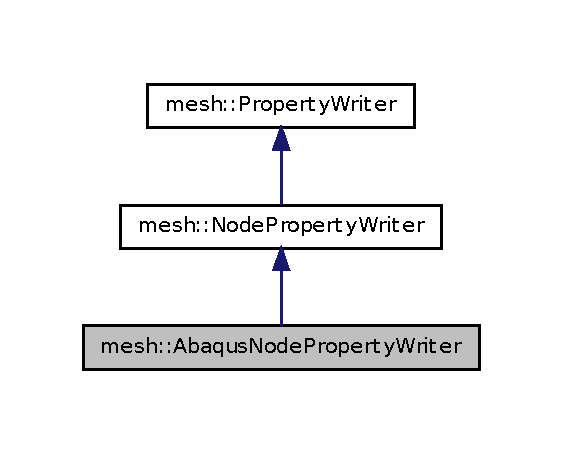
\includegraphics[width=270pt]{classmesh_1_1_abaqus_node_property_writer__inherit__graph}
\end{center}
\end{figure}


Collaboration diagram for mesh::AbaqusNodePropertyWriter:\nopagebreak
\begin{figure}[H]
\begin{center}
\leavevmode
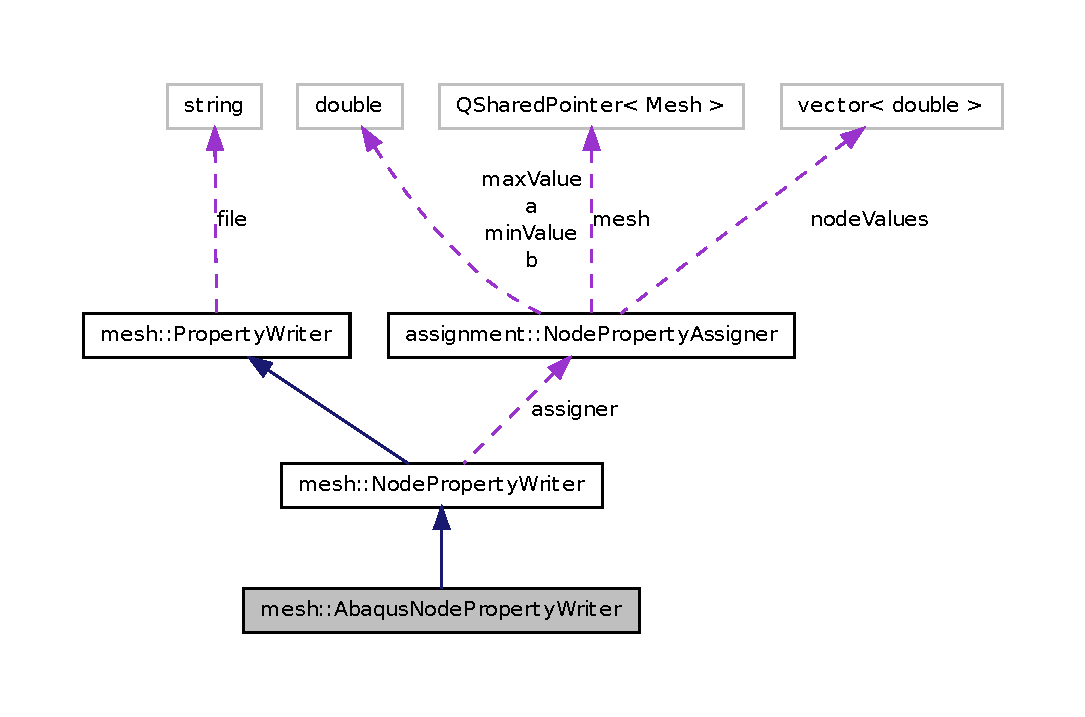
\includegraphics[width=400pt]{classmesh_1_1_abaqus_node_property_writer__coll__graph}
\end{center}
\end{figure}
\subsection*{Public Member Functions}
\begin{DoxyCompactItemize}
\item 
\hyperlink{classmesh_1_1_abaqus_node_property_writer_a6b69f1b093e673d2cbc6098ca5e0006b}{AbaqusNodePropertyWriter} (string \hyperlink{classmesh_1_1_property_writer_a296638bd6daba8a6545688bacfc4fef1}{file}, \hyperlink{classassignment_1_1_node_property_assigner}{NodePropertyAssigner} $\ast$\hyperlink{classmesh_1_1_node_property_writer_a3cfacf6c61f8f0131cc832f110526402}{assigner})
\begin{DoxyCompactList}\small\item\em Creates a new writer. \item\end{DoxyCompactList}\item 
\hypertarget{classmesh_1_1_abaqus_node_property_writer_a93dacc1b30500001ef87125322671e69}{
void \hyperlink{classmesh_1_1_abaqus_node_property_writer_a93dacc1b30500001ef87125322671e69}{write} ()}
\label{classmesh_1_1_abaqus_node_property_writer_a93dacc1b30500001ef87125322671e69}

\begin{DoxyCompactList}\small\item\em Writes the file. \item\end{DoxyCompactList}\end{DoxyCompactItemize}


\subsection{Detailed Description}
Writes a mesh file with node property assignment information to disk in Abaqus format. 

\subsection{Constructor \& Destructor Documentation}
\hypertarget{classmesh_1_1_abaqus_node_property_writer_a6b69f1b093e673d2cbc6098ca5e0006b}{
\index{mesh::AbaqusNodePropertyWriter@{mesh::AbaqusNodePropertyWriter}!AbaqusNodePropertyWriter@{AbaqusNodePropertyWriter}}
\index{AbaqusNodePropertyWriter@{AbaqusNodePropertyWriter}!mesh::AbaqusNodePropertyWriter@{mesh::AbaqusNodePropertyWriter}}
\subsubsection[{AbaqusNodePropertyWriter}]{\setlength{\rightskip}{0pt plus 5cm}mesh::AbaqusNodePropertyWriter::AbaqusNodePropertyWriter (
\begin{DoxyParamCaption}
\item[{string}]{ file, }
\item[{{\bf NodePropertyAssigner} $\ast$}]{ assigner}
\end{DoxyParamCaption}
)}}
\label{classmesh_1_1_abaqus_node_property_writer_a6b69f1b093e673d2cbc6098ca5e0006b}


Creates a new writer. 


\begin{DoxyParams}{Parameters}
\item[{\em file}]The file string \item[{\em assigner}]The \hyperlink{classassignment_1_1_node_property_assigner}{assignment::NodePropertyAssigner} \end{DoxyParams}


The documentation for this class was generated from the following files:\begin{DoxyCompactItemize}
\item 
mesh/AbaqusNodePropertyWriter.h\item 
mesh/AbaqusNodePropertyWriter.cxx\end{DoxyCompactItemize}

\hypertarget{classmesh_1_1_ansys_element_property_writer}{
\section{mesh::AnsysElementPropertyWriter Class Reference}
\label{classmesh_1_1_ansys_element_property_writer}\index{mesh::AnsysElementPropertyWriter@{mesh::AnsysElementPropertyWriter}}
}


Writes a mesh file with element property assignment information to disk in Ansys format.  




{\ttfamily \#include $<$AnsysElementPropertyWriter.h$>$}



Inheritance diagram for mesh::AnsysElementPropertyWriter:\nopagebreak
\begin{figure}[H]
\begin{center}
\leavevmode
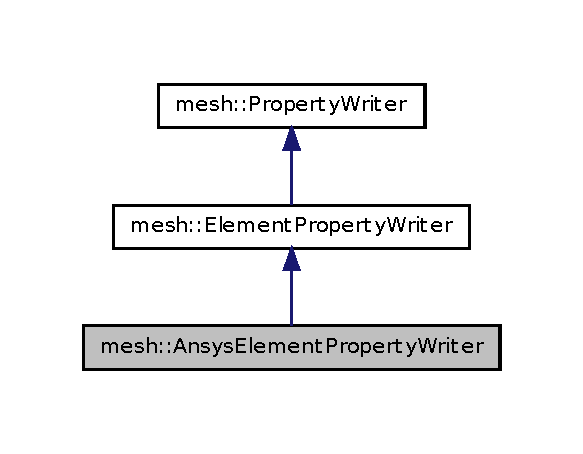
\includegraphics[width=280pt]{classmesh_1_1_ansys_element_property_writer__inherit__graph}
\end{center}
\end{figure}


Collaboration diagram for mesh::AnsysElementPropertyWriter:\nopagebreak
\begin{figure}[H]
\begin{center}
\leavevmode
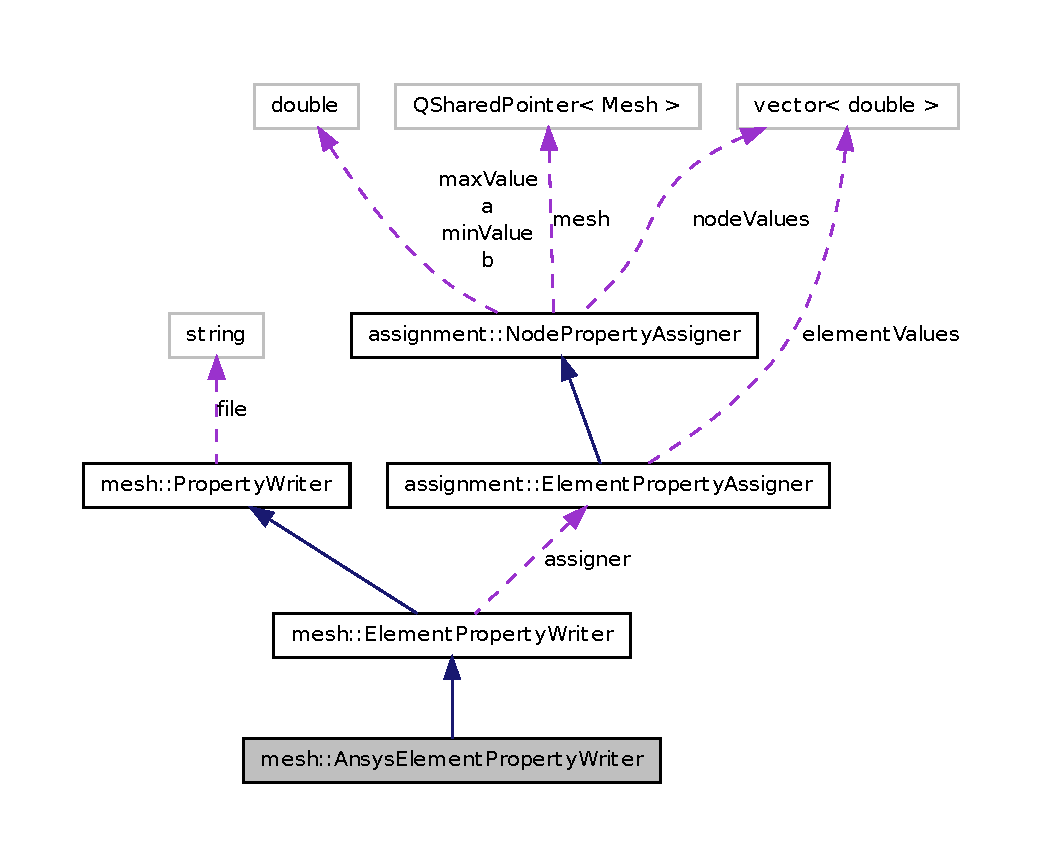
\includegraphics[width=400pt]{classmesh_1_1_ansys_element_property_writer__coll__graph}
\end{center}
\end{figure}
\subsection*{Public Member Functions}
\begin{DoxyCompactItemize}
\item 
\hyperlink{classmesh_1_1_ansys_element_property_writer_a6651a42e403a77c2f2d47aceaf63ed19}{AnsysElementPropertyWriter} (string \hyperlink{classmesh_1_1_property_writer_a296638bd6daba8a6545688bacfc4fef1}{file}, \hyperlink{classassignment_1_1_element_property_assigner}{assignment::ElementPropertyAssigner} $\ast$\hyperlink{classmesh_1_1_element_property_writer_a2b64c6f7960645dd64fa9e1e62f2ac10}{assigner})
\begin{DoxyCompactList}\small\item\em Creates a new writer. \item\end{DoxyCompactList}\item 
\hypertarget{classmesh_1_1_ansys_element_property_writer_a16a61f9efcc780e82ca37d034e4b84a6}{
void \hyperlink{classmesh_1_1_ansys_element_property_writer_a16a61f9efcc780e82ca37d034e4b84a6}{write} ()}
\label{classmesh_1_1_ansys_element_property_writer_a16a61f9efcc780e82ca37d034e4b84a6}

\begin{DoxyCompactList}\small\item\em Writes the file. \item\end{DoxyCompactList}\end{DoxyCompactItemize}


\subsection{Detailed Description}
Writes a mesh file with element property assignment information to disk in Ansys format. 

\subsection{Constructor \& Destructor Documentation}
\hypertarget{classmesh_1_1_ansys_element_property_writer_a6651a42e403a77c2f2d47aceaf63ed19}{
\index{mesh::AnsysElementPropertyWriter@{mesh::AnsysElementPropertyWriter}!AnsysElementPropertyWriter@{AnsysElementPropertyWriter}}
\index{AnsysElementPropertyWriter@{AnsysElementPropertyWriter}!mesh::AnsysElementPropertyWriter@{mesh::AnsysElementPropertyWriter}}
\subsubsection[{AnsysElementPropertyWriter}]{\setlength{\rightskip}{0pt plus 5cm}mesh::AnsysElementPropertyWriter::AnsysElementPropertyWriter (
\begin{DoxyParamCaption}
\item[{string}]{ file, }
\item[{{\bf assignment::ElementPropertyAssigner} $\ast$}]{ assigner}
\end{DoxyParamCaption}
)}}
\label{classmesh_1_1_ansys_element_property_writer_a6651a42e403a77c2f2d47aceaf63ed19}


Creates a new writer. 


\begin{DoxyParams}{Parameters}
\item[{\em file}]The file string \item[{\em assigner}]The \hyperlink{classassignment_1_1_element_property_assigner}{assignment::ElementPropertyAssigner} \end{DoxyParams}


The documentation for this class was generated from the following files:\begin{DoxyCompactItemize}
\item 
mesh/AnsysElementPropertyWriter.h\item 
mesh/AnsysElementPropertyWriter.cxx\end{DoxyCompactItemize}

\hypertarget{classmesh_1_1_ansys_mesh_loader}{
\section{mesh::AnsysMeshLoader Class Reference}
\label{classmesh_1_1_ansys_mesh_loader}\index{mesh::AnsysMeshLoader@{mesh::AnsysMeshLoader}}
}


Loads an Ansys mesh.  




{\ttfamily \#include $<$AnsysMeshLoader.h$>$}



Inheritance diagram for mesh::AnsysMeshLoader:\nopagebreak
\begin{figure}[H]
\begin{center}
\leavevmode
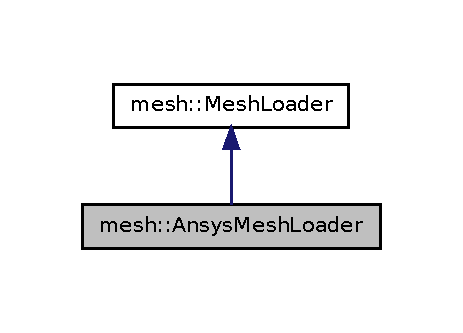
\includegraphics[width=222pt]{classmesh_1_1_ansys_mesh_loader__inherit__graph}
\end{center}
\end{figure}


Collaboration diagram for mesh::AnsysMeshLoader:\nopagebreak
\begin{figure}[H]
\begin{center}
\leavevmode
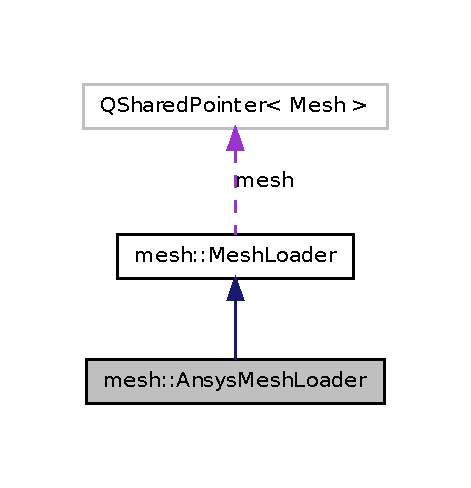
\includegraphics[width=226pt]{classmesh_1_1_ansys_mesh_loader__coll__graph}
\end{center}
\end{figure}
\subsection*{Public Member Functions}
\begin{DoxyCompactItemize}
\item 
\hyperlink{classmesh_1_1_ansys_mesh_loader_af00954f045eedef4afb90dd4efdde0bb}{AnsysMeshLoader} (string folder)
\begin{DoxyCompactList}\small\item\em Creates a new loader and reads from the specified Ansys folder. \item\end{DoxyCompactList}\end{DoxyCompactItemize}


\subsection{Detailed Description}
Loads an Ansys mesh. 

\subsection{Constructor \& Destructor Documentation}
\hypertarget{classmesh_1_1_ansys_mesh_loader_af00954f045eedef4afb90dd4efdde0bb}{
\index{mesh::AnsysMeshLoader@{mesh::AnsysMeshLoader}!AnsysMeshLoader@{AnsysMeshLoader}}
\index{AnsysMeshLoader@{AnsysMeshLoader}!mesh::AnsysMeshLoader@{mesh::AnsysMeshLoader}}
\subsubsection[{AnsysMeshLoader}]{\setlength{\rightskip}{0pt plus 5cm}mesh::AnsysMeshLoader::AnsysMeshLoader (
\begin{DoxyParamCaption}
\item[{string}]{ folder}
\end{DoxyParamCaption}
)}}
\label{classmesh_1_1_ansys_mesh_loader_af00954f045eedef4afb90dd4efdde0bb}


Creates a new loader and reads from the specified Ansys folder. 


\begin{DoxyParams}{Parameters}
\item[{\em folder}]The folder to the Ansys files \end{DoxyParams}


The documentation for this class was generated from the following files:\begin{DoxyCompactItemize}
\item 
mesh/AnsysMeshLoader.h\item 
mesh/AnsysMeshLoader.cxx\end{DoxyCompactItemize}

\hypertarget{classmesh_1_1_ansys_node_property_writer}{
\section{mesh::AnsysNodePropertyWriter Class Reference}
\label{classmesh_1_1_ansys_node_property_writer}\index{mesh::AnsysNodePropertyWriter@{mesh::AnsysNodePropertyWriter}}
}


Writes a mesh file with node property assignment information to disk in Ansys format.  




{\ttfamily \#include $<$AnsysNodePropertyWriter.h$>$}



Inheritance diagram for mesh::AnsysNodePropertyWriter:\nopagebreak
\begin{figure}[H]
\begin{center}
\leavevmode
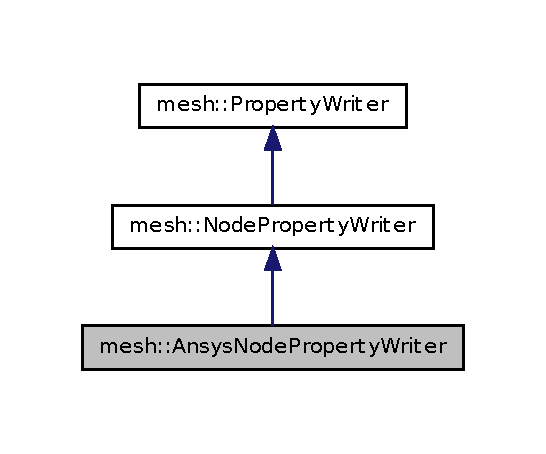
\includegraphics[width=262pt]{classmesh_1_1_ansys_node_property_writer__inherit__graph}
\end{center}
\end{figure}


Collaboration diagram for mesh::AnsysNodePropertyWriter:\nopagebreak
\begin{figure}[H]
\begin{center}
\leavevmode
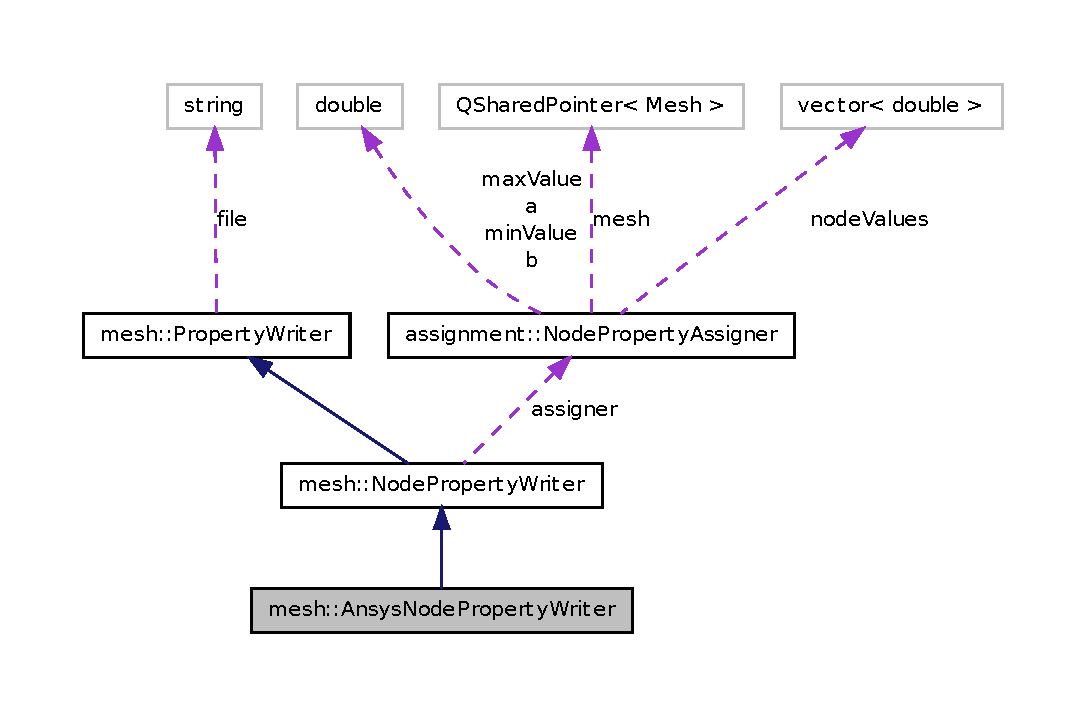
\includegraphics[width=400pt]{classmesh_1_1_ansys_node_property_writer__coll__graph}
\end{center}
\end{figure}
\subsection*{Public Member Functions}
\begin{DoxyCompactItemize}
\item 
\hyperlink{classmesh_1_1_ansys_node_property_writer_a54daf2c8746d4ffbb584752bf688fcf3}{AnsysNodePropertyWriter} (string \hyperlink{classmesh_1_1_property_writer_a296638bd6daba8a6545688bacfc4fef1}{file}, \hyperlink{classassignment_1_1_node_property_assigner}{NodePropertyAssigner} $\ast$\hyperlink{classmesh_1_1_node_property_writer_a3cfacf6c61f8f0131cc832f110526402}{assigner})
\begin{DoxyCompactList}\small\item\em Creates a new writer. \item\end{DoxyCompactList}\item 
\hypertarget{classmesh_1_1_ansys_node_property_writer_ad58fc51a2be4b9022191c6392c35227e}{
void \hyperlink{classmesh_1_1_ansys_node_property_writer_ad58fc51a2be4b9022191c6392c35227e}{write} ()}
\label{classmesh_1_1_ansys_node_property_writer_ad58fc51a2be4b9022191c6392c35227e}

\begin{DoxyCompactList}\small\item\em Writes the file. \item\end{DoxyCompactList}\end{DoxyCompactItemize}


\subsection{Detailed Description}
Writes a mesh file with node property assignment information to disk in Ansys format. 

\subsection{Constructor \& Destructor Documentation}
\hypertarget{classmesh_1_1_ansys_node_property_writer_a54daf2c8746d4ffbb584752bf688fcf3}{
\index{mesh::AnsysNodePropertyWriter@{mesh::AnsysNodePropertyWriter}!AnsysNodePropertyWriter@{AnsysNodePropertyWriter}}
\index{AnsysNodePropertyWriter@{AnsysNodePropertyWriter}!mesh::AnsysNodePropertyWriter@{mesh::AnsysNodePropertyWriter}}
\subsubsection[{AnsysNodePropertyWriter}]{\setlength{\rightskip}{0pt plus 5cm}mesh::AnsysNodePropertyWriter::AnsysNodePropertyWriter (
\begin{DoxyParamCaption}
\item[{string}]{ file, }
\item[{{\bf NodePropertyAssigner} $\ast$}]{ assigner}
\end{DoxyParamCaption}
)}}
\label{classmesh_1_1_ansys_node_property_writer_a54daf2c8746d4ffbb584752bf688fcf3}


Creates a new writer. 


\begin{DoxyParams}{Parameters}
\item[{\em file}]The file string \item[{\em assigner}]The \hyperlink{classassignment_1_1_node_property_assigner}{assignment::NodePropertyAssigner} \end{DoxyParams}


The documentation for this class was generated from the following files:\begin{DoxyCompactItemize}
\item 
mesh/AnsysNodePropertyWriter.h\item 
mesh/AnsysNodePropertyWriter.cxx\end{DoxyCompactItemize}

\hypertarget{classmesh_1_1_element_property_writer}{
\section{mesh::ElementPropertyWriter Class Reference}
\label{classmesh_1_1_element_property_writer}\index{mesh::ElementPropertyWriter@{mesh::ElementPropertyWriter}}
}


Abstract writer class to write a mesh file with element property assignment information to disk.  




{\ttfamily \#include $<$ElementPropertyWriter.h$>$}



Inheritance diagram for mesh::ElementPropertyWriter:\nopagebreak
\begin{figure}[H]
\begin{center}
\leavevmode
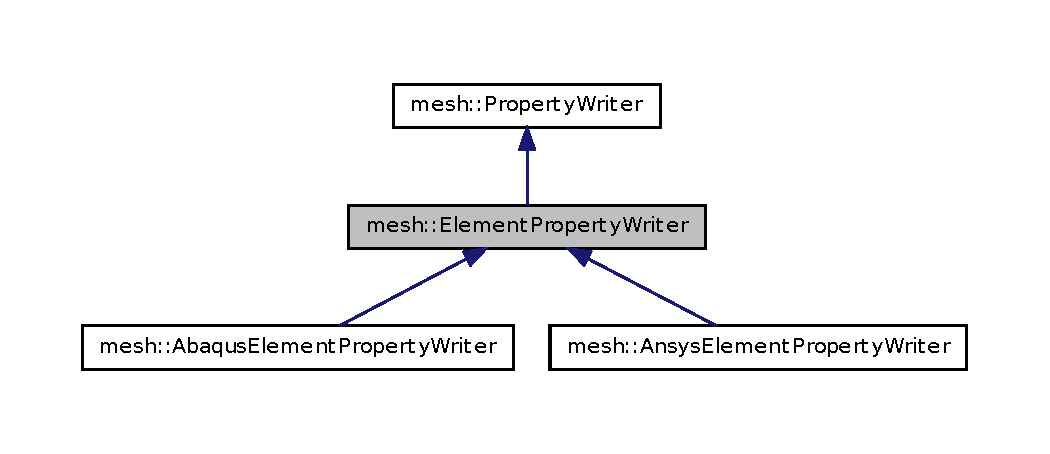
\includegraphics[width=400pt]{classmesh_1_1_element_property_writer__inherit__graph}
\end{center}
\end{figure}


Collaboration diagram for mesh::ElementPropertyWriter:\nopagebreak
\begin{figure}[H]
\begin{center}
\leavevmode
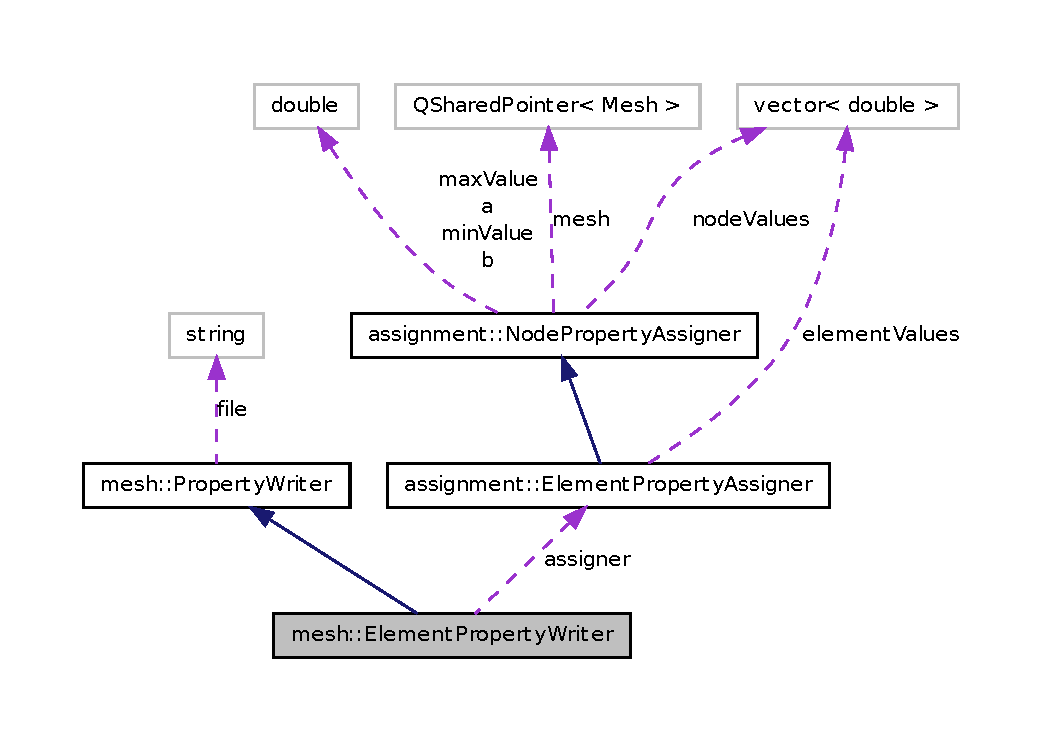
\includegraphics[width=400pt]{classmesh_1_1_element_property_writer__coll__graph}
\end{center}
\end{figure}
\subsection*{Public Member Functions}
\begin{DoxyCompactItemize}
\item 
\hyperlink{classmesh_1_1_element_property_writer_aacedd9047813db196c47855293c56acb}{ElementPropertyWriter} (string \hyperlink{classmesh_1_1_property_writer_a296638bd6daba8a6545688bacfc4fef1}{file}, \hyperlink{classassignment_1_1_element_property_assigner}{ElementPropertyAssigner} $\ast$\hyperlink{classmesh_1_1_element_property_writer_a2b64c6f7960645dd64fa9e1e62f2ac10}{assigner})
\begin{DoxyCompactList}\small\item\em Creates a new writer. \item\end{DoxyCompactList}\end{DoxyCompactItemize}
\subsection*{Protected Attributes}
\begin{DoxyCompactItemize}
\item 
\hypertarget{classmesh_1_1_element_property_writer_a2b64c6f7960645dd64fa9e1e62f2ac10}{
\hyperlink{classassignment_1_1_element_property_assigner}{ElementPropertyAssigner} $\ast$ \hyperlink{classmesh_1_1_element_property_writer_a2b64c6f7960645dd64fa9e1e62f2ac10}{assigner}}
\label{classmesh_1_1_element_property_writer_a2b64c6f7960645dd64fa9e1e62f2ac10}

\begin{DoxyCompactList}\small\item\em The assigner that was used for the assignment. \item\end{DoxyCompactList}\end{DoxyCompactItemize}


\subsection{Detailed Description}
Abstract writer class to write a mesh file with element property assignment information to disk. 

\subsection{Constructor \& Destructor Documentation}
\hypertarget{classmesh_1_1_element_property_writer_aacedd9047813db196c47855293c56acb}{
\index{mesh::ElementPropertyWriter@{mesh::ElementPropertyWriter}!ElementPropertyWriter@{ElementPropertyWriter}}
\index{ElementPropertyWriter@{ElementPropertyWriter}!mesh::ElementPropertyWriter@{mesh::ElementPropertyWriter}}
\subsubsection[{ElementPropertyWriter}]{\setlength{\rightskip}{0pt plus 5cm}mesh::ElementPropertyWriter::ElementPropertyWriter (
\begin{DoxyParamCaption}
\item[{string}]{ file, }
\item[{{\bf ElementPropertyAssigner} $\ast$}]{ assigner}
\end{DoxyParamCaption}
)}}
\label{classmesh_1_1_element_property_writer_aacedd9047813db196c47855293c56acb}


Creates a new writer. 


\begin{DoxyParams}{Parameters}
\item[{\em file}]The file string \item[{\em assigner}]The \hyperlink{classassignment_1_1_element_property_assigner}{assignment::ElementPropertyAssigner} \end{DoxyParams}


The documentation for this class was generated from the following files:\begin{DoxyCompactItemize}
\item 
mesh/ElementPropertyWriter.h\item 
mesh/ElementPropertyWriter.cxx\end{DoxyCompactItemize}

\hypertarget{structmesh_1_1_element_triangle}{
\section{mesh::ElementTriangle Struct Reference}
\label{structmesh_1_1_element_triangle}\index{mesh::ElementTriangle@{mesh::ElementTriangle}}
}


Collaboration diagram for mesh::ElementTriangle:\nopagebreak
\begin{figure}[H]
\begin{center}
\leavevmode
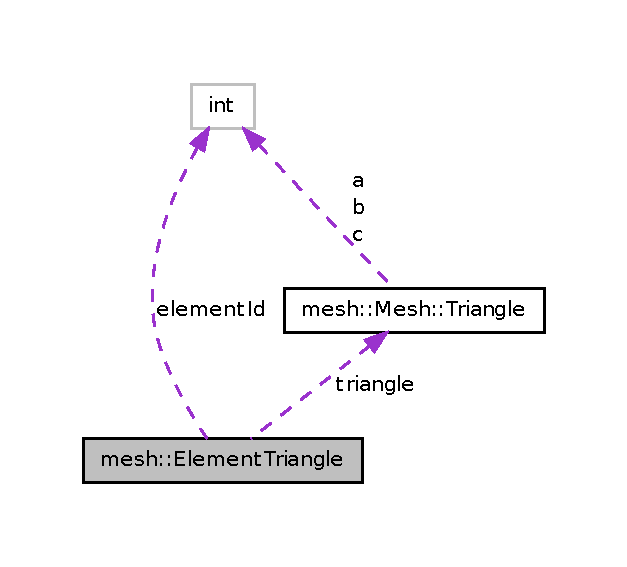
\includegraphics[width=301pt]{structmesh_1_1_element_triangle__coll__graph}
\end{center}
\end{figure}
\subsection*{Public Attributes}
\begin{DoxyCompactItemize}
\item 
\hypertarget{structmesh_1_1_element_triangle_aed9632916db442aea0edf3a1da8a1fad}{
int {\bfseries elementId}}
\label{structmesh_1_1_element_triangle_aed9632916db442aea0edf3a1da8a1fad}

\item 
\hypertarget{structmesh_1_1_element_triangle_a9b8df40432def8b3b715e01f8706df0e}{
\hyperlink{structmesh_1_1_mesh_1_1_triangle}{Mesh::Triangle} {\bfseries triangle}}
\label{structmesh_1_1_element_triangle_a9b8df40432def8b3b715e01f8706df0e}

\end{DoxyCompactItemize}


The documentation for this struct was generated from the following file:\begin{DoxyCompactItemize}
\item 
mesh/AbaqusMeshLoader.cxx\end{DoxyCompactItemize}

\hypertarget{classmesh_1_1_mesh}{
\section{mesh::Mesh Class Reference}
\label{classmesh_1_1_mesh}\index{mesh::Mesh@{mesh::Mesh}}
}


This class holds mesh data.  




{\ttfamily \#include $<$Mesh.h$>$}



Collaboration diagram for mesh::Mesh:\nopagebreak
\begin{figure}[H]
\begin{center}
\leavevmode
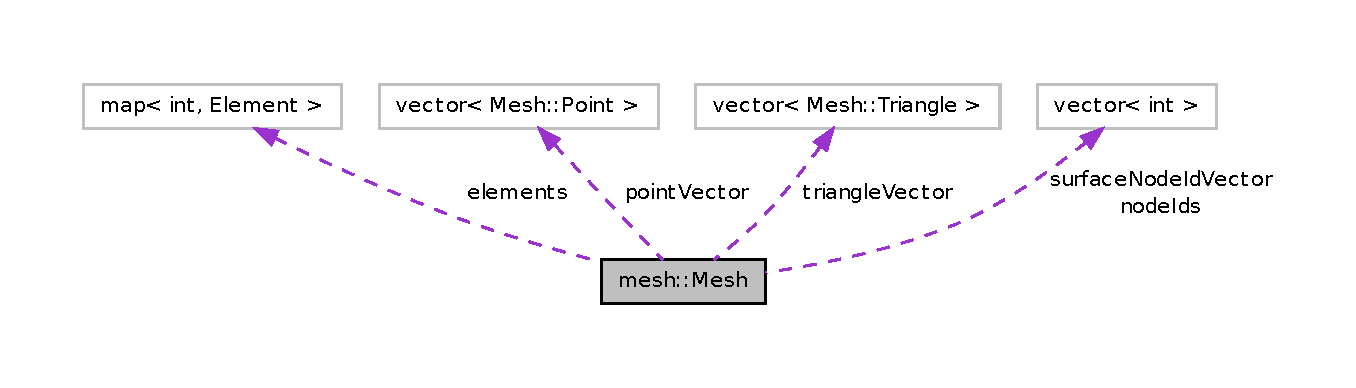
\includegraphics[width=400pt]{classmesh_1_1_mesh__coll__graph}
\end{center}
\end{figure}
\subsection*{Classes}
\begin{DoxyCompactItemize}
\item 
struct \hyperlink{structmesh_1_1_mesh_1_1_element}{Element}
\begin{DoxyCompactList}\small\item\em An element with its node Ids. \item\end{DoxyCompactList}\item 
struct \hyperlink{structmesh_1_1_mesh_1_1_point}{Point}
\begin{DoxyCompactList}\small\item\em A point in space. \item\end{DoxyCompactList}\item 
struct \hyperlink{structmesh_1_1_mesh_1_1_triangle}{Triangle}
\begin{DoxyCompactList}\small\item\em A surface triangle of three node Ids. \item\end{DoxyCompactList}\end{DoxyCompactItemize}
\subsection*{Public Member Functions}
\begin{DoxyCompactItemize}
\item 
vector$<$ int $>$ $\ast$ \hyperlink{classmesh_1_1_mesh_a08b9ef9ed39c4252d8c5819d527b4bb5}{getNodeIds} ()
\item 
vector$<$ \hyperlink{structmesh_1_1_mesh_1_1_triangle}{Mesh::Triangle} $>$ $\ast$ \hyperlink{classmesh_1_1_mesh_adea40edfe5208ed0635d01319305a52b}{getTriangleVector} ()
\item 
vector$<$ \hyperlink{structmesh_1_1_mesh_1_1_point}{Mesh::Point} $>$ $\ast$ \hyperlink{classmesh_1_1_mesh_aee129b99bbc5ed1fc69c4b35be8e9536}{getPointVector} ()
\item 
map$<$ int, \hyperlink{structmesh_1_1_mesh_1_1_element}{Element} $>$ $\ast$ \hyperlink{classmesh_1_1_mesh_a5b766d9061fcc7ee30d6b0059cfa815f}{getElements} ()
\end{DoxyCompactItemize}
\subsection*{Protected Attributes}
\begin{DoxyCompactItemize}
\item 
\hypertarget{classmesh_1_1_mesh_ac32a7d59a92de7a1e4eaf5b016d63dff}{
vector$<$ int $>$ \hyperlink{classmesh_1_1_mesh_ac32a7d59a92de7a1e4eaf5b016d63dff}{surfaceNodeIdVector}}
\label{classmesh_1_1_mesh_ac32a7d59a92de7a1e4eaf5b016d63dff}

\begin{DoxyCompactList}\small\item\em The surface node Ids. \item\end{DoxyCompactList}\item 
\hypertarget{classmesh_1_1_mesh_acdbed9293a87ffde0887764db16809ef}{
vector$<$ \hyperlink{structmesh_1_1_mesh_1_1_triangle}{Mesh::Triangle} $>$ \hyperlink{classmesh_1_1_mesh_acdbed9293a87ffde0887764db16809ef}{triangleVector}}
\label{classmesh_1_1_mesh_acdbed9293a87ffde0887764db16809ef}

\begin{DoxyCompactList}\small\item\em The surface triangles. \item\end{DoxyCompactList}\item 
\hypertarget{classmesh_1_1_mesh_a1caa15084eed4de46071cdb1da774069}{
vector$<$ int $>$ \hyperlink{classmesh_1_1_mesh_a1caa15084eed4de46071cdb1da774069}{nodeIds}}
\label{classmesh_1_1_mesh_a1caa15084eed4de46071cdb1da774069}

\begin{DoxyCompactList}\small\item\em The node Ids. \item\end{DoxyCompactList}\item 
\hypertarget{classmesh_1_1_mesh_ac004fba269ab0a78d688360865d5ae1a}{
vector$<$ \hyperlink{structmesh_1_1_mesh_1_1_point}{Mesh::Point} $>$ \hyperlink{classmesh_1_1_mesh_ac004fba269ab0a78d688360865d5ae1a}{pointVector}}
\label{classmesh_1_1_mesh_ac004fba269ab0a78d688360865d5ae1a}

\begin{DoxyCompactList}\small\item\em The node coordinates. \item\end{DoxyCompactList}\item 
\hypertarget{classmesh_1_1_mesh_a96bc5c338398ead84b1ab2aa9b664d06}{
map$<$ int, \hyperlink{structmesh_1_1_mesh_1_1_element}{Element} $>$ \hyperlink{classmesh_1_1_mesh_a96bc5c338398ead84b1ab2aa9b664d06}{elements}}
\label{classmesh_1_1_mesh_a96bc5c338398ead84b1ab2aa9b664d06}

\begin{DoxyCompactList}\small\item\em A map that maps the element Ids to the \hyperlink{structmesh_1_1_mesh_1_1_element}{mesh::Mesh::Element} data. \item\end{DoxyCompactList}\end{DoxyCompactItemize}
\subsection*{Friends}
\begin{DoxyCompactItemize}
\item 
\hypertarget{classmesh_1_1_mesh_a5da36615b6c00ca1941e7504222978be}{
class {\bfseries AnsysMeshLoader}}
\label{classmesh_1_1_mesh_a5da36615b6c00ca1941e7504222978be}

\item 
\hypertarget{classmesh_1_1_mesh_a7b065f6fb884c97bbb9100e204979c70}{
class {\bfseries AbaqusMeshLoader}}
\label{classmesh_1_1_mesh_a7b065f6fb884c97bbb9100e204979c70}

\end{DoxyCompactItemize}


\subsection{Detailed Description}
This class holds mesh data. 

\subsection{Member Function Documentation}
\hypertarget{classmesh_1_1_mesh_a5b766d9061fcc7ee30d6b0059cfa815f}{
\index{mesh::Mesh@{mesh::Mesh}!getElements@{getElements}}
\index{getElements@{getElements}!mesh::Mesh@{mesh::Mesh}}
\subsubsection[{getElements}]{\setlength{\rightskip}{0pt plus 5cm}map$<$ int, {\bf Mesh::Element} $>$ $\ast$ mesh::Mesh::getElements (
\begin{DoxyParamCaption}
{}
\end{DoxyParamCaption}
)}}
\label{classmesh_1_1_mesh_a5b766d9061fcc7ee30d6b0059cfa815f}
\begin{DoxyReturn}{Returns}
The map that maps the element Ids to the \hyperlink{structmesh_1_1_mesh_1_1_element}{mesh::Mesh::Element} data 
\end{DoxyReturn}
\hypertarget{classmesh_1_1_mesh_a08b9ef9ed39c4252d8c5819d527b4bb5}{
\index{mesh::Mesh@{mesh::Mesh}!getNodeIds@{getNodeIds}}
\index{getNodeIds@{getNodeIds}!mesh::Mesh@{mesh::Mesh}}
\subsubsection[{getNodeIds}]{\setlength{\rightskip}{0pt plus 5cm}vector$<$ int $>$ $\ast$ mesh::Mesh::getNodeIds (
\begin{DoxyParamCaption}
{}
\end{DoxyParamCaption}
)}}
\label{classmesh_1_1_mesh_a08b9ef9ed39c4252d8c5819d527b4bb5}
\begin{DoxyReturn}{Returns}
The node Ids 
\end{DoxyReturn}
\hypertarget{classmesh_1_1_mesh_aee129b99bbc5ed1fc69c4b35be8e9536}{
\index{mesh::Mesh@{mesh::Mesh}!getPointVector@{getPointVector}}
\index{getPointVector@{getPointVector}!mesh::Mesh@{mesh::Mesh}}
\subsubsection[{getPointVector}]{\setlength{\rightskip}{0pt plus 5cm}vector$<$ {\bf Mesh::Point} $>$ $\ast$ mesh::Mesh::getPointVector (
\begin{DoxyParamCaption}
{}
\end{DoxyParamCaption}
)}}
\label{classmesh_1_1_mesh_aee129b99bbc5ed1fc69c4b35be8e9536}
\begin{DoxyReturn}{Returns}
The node coordinates 
\end{DoxyReturn}
\hypertarget{classmesh_1_1_mesh_adea40edfe5208ed0635d01319305a52b}{
\index{mesh::Mesh@{mesh::Mesh}!getTriangleVector@{getTriangleVector}}
\index{getTriangleVector@{getTriangleVector}!mesh::Mesh@{mesh::Mesh}}
\subsubsection[{getTriangleVector}]{\setlength{\rightskip}{0pt plus 5cm}vector$<$ {\bf Mesh::Triangle} $>$ $\ast$ mesh::Mesh::getTriangleVector (
\begin{DoxyParamCaption}
{}
\end{DoxyParamCaption}
)}}
\label{classmesh_1_1_mesh_adea40edfe5208ed0635d01319305a52b}
\begin{DoxyReturn}{Returns}
The surface triangles 
\end{DoxyReturn}


The documentation for this class was generated from the following files:\begin{DoxyCompactItemize}
\item 
mesh/Mesh.h\item 
mesh/Mesh.cxx\end{DoxyCompactItemize}

\hypertarget{structmesh_1_1_mesh_1_1_element}{
\section{mesh::Mesh::Element Struct Reference}
\label{structmesh_1_1_mesh_1_1_element}\index{mesh::Mesh::Element@{mesh::Mesh::Element}}
}


An element with its node Ids.  




{\ttfamily \#include $<$Mesh.h$>$}



Collaboration diagram for mesh::Mesh::Element:\nopagebreak
\begin{figure}[H]
\begin{center}
\leavevmode
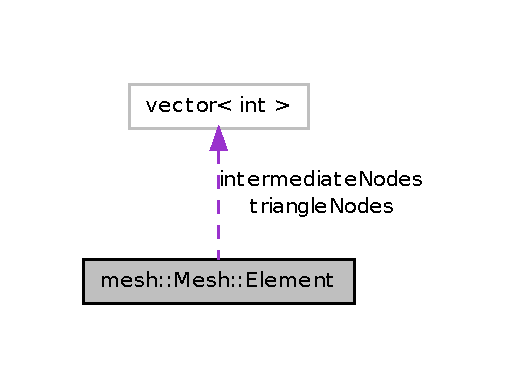
\includegraphics[width=244pt]{structmesh_1_1_mesh_1_1_element__coll__graph}
\end{center}
\end{figure}
\subsection*{Public Attributes}
\begin{DoxyCompactItemize}
\item 
\hypertarget{structmesh_1_1_mesh_1_1_element_aaf33edc392c36b6be1757b42759c5392}{
vector$<$ int $>$ {\bfseries triangleNodes}}
\label{structmesh_1_1_mesh_1_1_element_aaf33edc392c36b6be1757b42759c5392}

\item 
\hypertarget{structmesh_1_1_mesh_1_1_element_a5cba271f3a925ae2567080b85f5d05b4}{
vector$<$ int $>$ {\bfseries intermediateNodes}}
\label{structmesh_1_1_mesh_1_1_element_a5cba271f3a925ae2567080b85f5d05b4}

\end{DoxyCompactItemize}


\subsection{Detailed Description}
An element with its node Ids. 

The documentation for this struct was generated from the following file:\begin{DoxyCompactItemize}
\item 
mesh/Mesh.h\end{DoxyCompactItemize}

\hypertarget{structmesh_1_1_mesh_1_1_point}{
\section{mesh::Mesh::Point Struct Reference}
\label{structmesh_1_1_mesh_1_1_point}\index{mesh::Mesh::Point@{mesh::Mesh::Point}}
}


A point in space.  




{\ttfamily \#include $<$Mesh.h$>$}



Collaboration diagram for mesh::Mesh::Point:\nopagebreak
\begin{figure}[H]
\begin{center}
\leavevmode
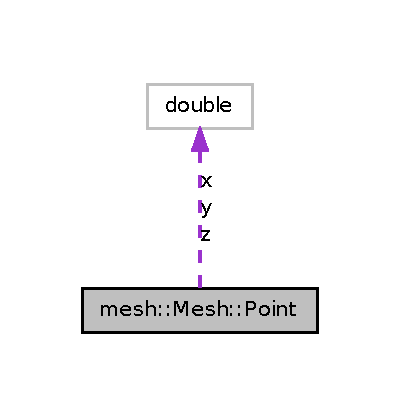
\includegraphics[width=192pt]{structmesh_1_1_mesh_1_1_point__coll__graph}
\end{center}
\end{figure}
\subsection*{Public Attributes}
\begin{DoxyCompactItemize}
\item 
\hypertarget{structmesh_1_1_mesh_1_1_point_ae152ff4a904b2456fa625b4b88558d02}{
double {\bfseries x}}
\label{structmesh_1_1_mesh_1_1_point_ae152ff4a904b2456fa625b4b88558d02}

\item 
\hypertarget{structmesh_1_1_mesh_1_1_point_a04ba06eed96be76e338c9b03f4205e44}{
double {\bfseries y}}
\label{structmesh_1_1_mesh_1_1_point_a04ba06eed96be76e338c9b03f4205e44}

\item 
\hypertarget{structmesh_1_1_mesh_1_1_point_a8521a63f6c7f4ec8290b9e8f6205c410}{
double {\bfseries z}}
\label{structmesh_1_1_mesh_1_1_point_a8521a63f6c7f4ec8290b9e8f6205c410}

\end{DoxyCompactItemize}


\subsection{Detailed Description}
A point in space. 

The documentation for this struct was generated from the following file:\begin{DoxyCompactItemize}
\item 
mesh/Mesh.h\end{DoxyCompactItemize}

\hypertarget{structmesh_1_1_mesh_1_1_triangle}{
\section{mesh::Mesh::Triangle Struct Reference}
\label{structmesh_1_1_mesh_1_1_triangle}\index{mesh::Mesh::Triangle@{mesh::Mesh::Triangle}}
}


A surface triangle of three node Ids.  




{\ttfamily \#include $<$Mesh.h$>$}



Collaboration diagram for mesh::Mesh::Triangle:\nopagebreak
\begin{figure}[H]
\begin{center}
\leavevmode
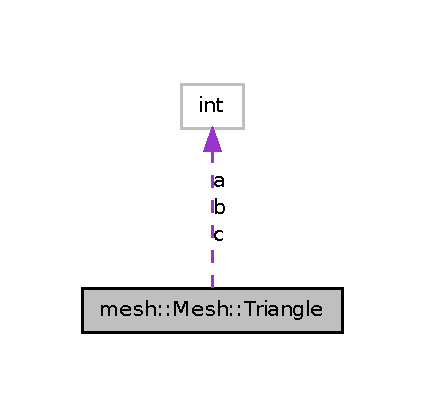
\includegraphics[width=204pt]{structmesh_1_1_mesh_1_1_triangle__coll__graph}
\end{center}
\end{figure}
\subsection*{Public Attributes}
\begin{DoxyCompactItemize}
\item 
\hypertarget{structmesh_1_1_mesh_1_1_triangle_af6f29d96acfd44f49ea9a848a057085b}{
int {\bfseries a}}
\label{structmesh_1_1_mesh_1_1_triangle_af6f29d96acfd44f49ea9a848a057085b}

\item 
\hypertarget{structmesh_1_1_mesh_1_1_triangle_aa94b0cfa8497c59eb3fae0afc32e7b0c}{
int {\bfseries b}}
\label{structmesh_1_1_mesh_1_1_triangle_aa94b0cfa8497c59eb3fae0afc32e7b0c}

\item 
\hypertarget{structmesh_1_1_mesh_1_1_triangle_ad9ad7d8be602ea8e822e05a1ba4f2bc7}{
int {\bfseries c}}
\label{structmesh_1_1_mesh_1_1_triangle_ad9ad7d8be602ea8e822e05a1ba4f2bc7}

\end{DoxyCompactItemize}


\subsection{Detailed Description}
A surface triangle of three node Ids. 

The documentation for this struct was generated from the following file:\begin{DoxyCompactItemize}
\item 
mesh/Mesh.h\end{DoxyCompactItemize}

\hypertarget{classmesh_1_1_mesh_loader}{
\section{mesh::MeshLoader Class Reference}
\label{classmesh_1_1_mesh_loader}\index{mesh::MeshLoader@{mesh::MeshLoader}}
}


Loads a mesh from disk.  




{\ttfamily \#include $<$MeshLoader.h$>$}



Inheritance diagram for mesh::MeshLoader:\nopagebreak
\begin{figure}[H]
\begin{center}
\leavevmode
\includegraphics[width=388pt]{classmesh_1_1_mesh_loader__inherit__graph}
\end{center}
\end{figure}


Collaboration diagram for mesh::MeshLoader:\nopagebreak
\begin{figure}[H]
\begin{center}
\leavevmode
\includegraphics[width=226pt]{classmesh_1_1_mesh_loader__coll__graph}
\end{center}
\end{figure}
\subsection*{Public Member Functions}
\begin{DoxyCompactItemize}
\item 
QSharedPointer$<$ \hyperlink{classmesh_1_1_mesh}{Mesh} $>$ \hyperlink{classmesh_1_1_mesh_loader_a9756af06988db1e1e4a1d8ad1c44b719}{getMesh} ()
\begin{DoxyCompactList}\small\item\em Gets the loaded \hyperlink{classmesh_1_1_mesh}{mesh::Mesh}. \item\end{DoxyCompactList}\end{DoxyCompactItemize}
\subsection*{Protected Attributes}
\begin{DoxyCompactItemize}
\item 
\hypertarget{classmesh_1_1_mesh_loader_a93f1f94c34ec2e114ea5414483349288}{
QSharedPointer$<$ \hyperlink{classmesh_1_1_mesh}{Mesh} $>$ \hyperlink{classmesh_1_1_mesh_loader_a93f1f94c34ec2e114ea5414483349288}{mesh}}
\label{classmesh_1_1_mesh_loader_a93f1f94c34ec2e114ea5414483349288}

\begin{DoxyCompactList}\small\item\em The laoded \hyperlink{classmesh_1_1_mesh}{mesh::Mesh}. \item\end{DoxyCompactList}\end{DoxyCompactItemize}


\subsection{Detailed Description}
Loads a mesh from disk. 

\subsection{Member Function Documentation}
\hypertarget{classmesh_1_1_mesh_loader_a9756af06988db1e1e4a1d8ad1c44b719}{
\index{mesh::MeshLoader@{mesh::MeshLoader}!getMesh@{getMesh}}
\index{getMesh@{getMesh}!mesh::MeshLoader@{mesh::MeshLoader}}
\subsubsection[{getMesh}]{\setlength{\rightskip}{0pt plus 5cm}QSharedPointer$<$ {\bf Mesh} $>$ mesh::MeshLoader::getMesh (
\begin{DoxyParamCaption}
{}
\end{DoxyParamCaption}
)}}
\label{classmesh_1_1_mesh_loader_a9756af06988db1e1e4a1d8ad1c44b719}


Gets the loaded \hyperlink{classmesh_1_1_mesh}{mesh::Mesh}. 

\begin{DoxyReturn}{Returns}
The loaded \hyperlink{classmesh_1_1_mesh}{mesh::Mesh} 
\end{DoxyReturn}


The documentation for this class was generated from the following files:\begin{DoxyCompactItemize}
\item 
mesh/MeshLoader.h\item 
mesh/MeshLoader.cxx\end{DoxyCompactItemize}

\hypertarget{classmesh_1_1_node_property_writer}{
\section{mesh::NodePropertyWriter Class Reference}
\label{classmesh_1_1_node_property_writer}\index{mesh::NodePropertyWriter@{mesh::NodePropertyWriter}}
}


Abstract writer class to write a mesh file with node property assignment information to disk.  




{\ttfamily \#include $<$NodePropertyWriter.h$>$}



Inheritance diagram for mesh::NodePropertyWriter:\nopagebreak
\begin{figure}[H]
\begin{center}
\leavevmode
\includegraphics[width=400pt]{classmesh_1_1_node_property_writer__inherit__graph}
\end{center}
\end{figure}


Collaboration diagram for mesh::NodePropertyWriter:\nopagebreak
\begin{figure}[H]
\begin{center}
\leavevmode
\includegraphics[width=400pt]{classmesh_1_1_node_property_writer__coll__graph}
\end{center}
\end{figure}
\subsection*{Public Member Functions}
\begin{DoxyCompactItemize}
\item 
\hyperlink{classmesh_1_1_node_property_writer_a973c19fe472c306c9d970a012d4e2137}{NodePropertyWriter} (string \hyperlink{classmesh_1_1_property_writer_a296638bd6daba8a6545688bacfc4fef1}{file}, \hyperlink{classassignment_1_1_node_property_assigner}{NodePropertyAssigner} $\ast$\hyperlink{classmesh_1_1_node_property_writer_a3cfacf6c61f8f0131cc832f110526402}{assigner})
\begin{DoxyCompactList}\small\item\em Creates a new writer. \item\end{DoxyCompactList}\end{DoxyCompactItemize}
\subsection*{Protected Attributes}
\begin{DoxyCompactItemize}
\item 
\hypertarget{classmesh_1_1_node_property_writer_a3cfacf6c61f8f0131cc832f110526402}{
\hyperlink{classassignment_1_1_node_property_assigner}{NodePropertyAssigner} $\ast$ \hyperlink{classmesh_1_1_node_property_writer_a3cfacf6c61f8f0131cc832f110526402}{assigner}}
\label{classmesh_1_1_node_property_writer_a3cfacf6c61f8f0131cc832f110526402}

\begin{DoxyCompactList}\small\item\em The assigner that was used for the assignment. \item\end{DoxyCompactList}\end{DoxyCompactItemize}


\subsection{Detailed Description}
Abstract writer class to write a mesh file with node property assignment information to disk. 

\subsection{Constructor \& Destructor Documentation}
\hypertarget{classmesh_1_1_node_property_writer_a973c19fe472c306c9d970a012d4e2137}{
\index{mesh::NodePropertyWriter@{mesh::NodePropertyWriter}!NodePropertyWriter@{NodePropertyWriter}}
\index{NodePropertyWriter@{NodePropertyWriter}!mesh::NodePropertyWriter@{mesh::NodePropertyWriter}}
\subsubsection[{NodePropertyWriter}]{\setlength{\rightskip}{0pt plus 5cm}mesh::NodePropertyWriter::NodePropertyWriter (
\begin{DoxyParamCaption}
\item[{string}]{ file, }
\item[{{\bf NodePropertyAssigner} $\ast$}]{ assigner}
\end{DoxyParamCaption}
)}}
\label{classmesh_1_1_node_property_writer_a973c19fe472c306c9d970a012d4e2137}


Creates a new writer. 


\begin{DoxyParams}{Parameters}
\item[{\em file}]The file string \item[{\em assigner}]The \hyperlink{classassignment_1_1_node_property_assigner}{assignment::NodePropertyAssigner} \end{DoxyParams}


The documentation for this class was generated from the following files:\begin{DoxyCompactItemize}
\item 
mesh/NodePropertyWriter.h\item 
mesh/NodePropertyWriter.cxx\end{DoxyCompactItemize}

\hypertarget{classmesh_1_1_property_writer}{
\section{mesh::PropertyWriter Class Reference}
\label{classmesh_1_1_property_writer}\index{mesh::PropertyWriter@{mesh::PropertyWriter}}
}


Abstract writer class to write a mesh file with property assignment information to disk.  




{\ttfamily \#include $<$PropertyWriter.h$>$}



Inheritance diagram for mesh::PropertyWriter:\nopagebreak
\begin{figure}[H]
\begin{center}
\leavevmode
\includegraphics[width=400pt]{classmesh_1_1_property_writer__inherit__graph}
\end{center}
\end{figure}


Collaboration diagram for mesh::PropertyWriter:\nopagebreak
\begin{figure}[H]
\begin{center}
\leavevmode
\includegraphics[width=208pt]{classmesh_1_1_property_writer__coll__graph}
\end{center}
\end{figure}
\subsection*{Public Member Functions}
\begin{DoxyCompactItemize}
\item 
\hyperlink{classmesh_1_1_property_writer_a978874a41f62868cc2b1ba5d16256bdf}{PropertyWriter} (string \hyperlink{classmesh_1_1_property_writer_a296638bd6daba8a6545688bacfc4fef1}{file})
\begin{DoxyCompactList}\small\item\em Creates a new writer. \item\end{DoxyCompactList}\item 
\hypertarget{classmesh_1_1_property_writer_ab95dbcb397acfca04b34f3d677b734e5}{
virtual void \hyperlink{classmesh_1_1_property_writer_ab95dbcb397acfca04b34f3d677b734e5}{write} ()=0}
\label{classmesh_1_1_property_writer_ab95dbcb397acfca04b34f3d677b734e5}

\begin{DoxyCompactList}\small\item\em Writes the file. \item\end{DoxyCompactList}\end{DoxyCompactItemize}
\subsection*{Protected Attributes}
\begin{DoxyCompactItemize}
\item 
\hypertarget{classmesh_1_1_property_writer_a296638bd6daba8a6545688bacfc4fef1}{
string \hyperlink{classmesh_1_1_property_writer_a296638bd6daba8a6545688bacfc4fef1}{file}}
\label{classmesh_1_1_property_writer_a296638bd6daba8a6545688bacfc4fef1}

\begin{DoxyCompactList}\small\item\em The file string. \item\end{DoxyCompactList}\end{DoxyCompactItemize}


\subsection{Detailed Description}
Abstract writer class to write a mesh file with property assignment information to disk. 

\subsection{Constructor \& Destructor Documentation}
\hypertarget{classmesh_1_1_property_writer_a978874a41f62868cc2b1ba5d16256bdf}{
\index{mesh::PropertyWriter@{mesh::PropertyWriter}!PropertyWriter@{PropertyWriter}}
\index{PropertyWriter@{PropertyWriter}!mesh::PropertyWriter@{mesh::PropertyWriter}}
\subsubsection[{PropertyWriter}]{\setlength{\rightskip}{0pt plus 5cm}mesh::PropertyWriter::PropertyWriter (
\begin{DoxyParamCaption}
\item[{string}]{ file}
\end{DoxyParamCaption}
)}}
\label{classmesh_1_1_property_writer_a978874a41f62868cc2b1ba5d16256bdf}


Creates a new writer. 


\begin{DoxyParams}{Parameters}
\item[{\em file}]The file string representing a file on disk \end{DoxyParams}


The documentation for this class was generated from the following files:\begin{DoxyCompactItemize}
\item 
mesh/PropertyWriter.h\item 
mesh/PropertyWriter.cxx\end{DoxyCompactItemize}

\hypertarget{class_process_object}{
\section{ProcessObject Class Reference}
\label{class_process_object}\index{ProcessObject@{ProcessObject}}
}


Inheritance diagram for ProcessObject:\nopagebreak
\begin{figure}[H]
\begin{center}
\leavevmode
\includegraphics[width=322pt]{class_process_object__inherit__graph}
\end{center}
\end{figure}


The documentation for this class was generated from the following file:\begin{DoxyCompactItemize}
\item 
itkImageToVTKImageFilter.h\end{DoxyCompactItemize}

\hypertarget{class_q_main_window}{
\section{QMainWindow Class Reference}
\label{class_q_main_window}\index{QMainWindow@{QMainWindow}}
}


Inheritance diagram for QMainWindow:\nopagebreak
\begin{figure}[H]
\begin{center}
\leavevmode
\includegraphics[width=180pt]{class_q_main_window__inherit__graph}
\end{center}
\end{figure}


The documentation for this class was generated from the following file:\begin{DoxyCompactItemize}
\item 
gui/MainWindow.h\end{DoxyCompactItemize}

\hypertarget{classtest_1_1_assignment_test}{
\section{test::AssignmentTest Class Reference}
\label{classtest_1_1_assignment_test}\index{test::AssignmentTest@{test::AssignmentTest}}
}


Inheritance diagram for test::AssignmentTest:\nopagebreak
\begin{figure}[H]
\begin{center}
\leavevmode
\includegraphics[width=208pt]{classtest_1_1_assignment_test__inherit__graph}
\end{center}
\end{figure}


Collaboration diagram for test::AssignmentTest:\nopagebreak
\begin{figure}[H]
\begin{center}
\leavevmode
\includegraphics[width=208pt]{classtest_1_1_assignment_test__coll__graph}
\end{center}
\end{figure}
\subsection*{Public Member Functions}
\begin{DoxyCompactItemize}
\item 
\hypertarget{classtest_1_1_assignment_test_aa6d17a10c5a139e78587929bc42b5a75}{
char $\ast$ {\bfseries run} ()}
\label{classtest_1_1_assignment_test_aa6d17a10c5a139e78587929bc42b5a75}

\end{DoxyCompactItemize}


The documentation for this class was generated from the following files:\begin{DoxyCompactItemize}
\item 
test/AssignmentTest.h\item 
test/AssignmentTest.cxx\end{DoxyCompactItemize}

\hypertarget{classtest_1_1_c_t_image_mock}{
\section{test::CTImageMock Class Reference}
\label{classtest_1_1_c_t_image_mock}\index{test::CTImageMock@{test::CTImageMock}}
}


Inheritance diagram for test::CTImageMock:\nopagebreak
\begin{figure}[H]
\begin{center}
\leavevmode
\includegraphics[width=198pt]{classtest_1_1_c_t_image_mock__inherit__graph}
\end{center}
\end{figure}


Collaboration diagram for test::CTImageMock:\nopagebreak
\begin{figure}[H]
\begin{center}
\leavevmode
\includegraphics[width=375pt]{classtest_1_1_c_t_image_mock__coll__graph}
\end{center}
\end{figure}


The documentation for this class was generated from the following files:\begin{DoxyCompactItemize}
\item 
test/CTImageMock.h\item 
test/CTImageMock.cxx\end{DoxyCompactItemize}

\hypertarget{classtest_1_1_c_t_image_test}{
\section{test::CTImageTest Class Reference}
\label{classtest_1_1_c_t_image_test}\index{test::CTImageTest@{test::CTImageTest}}
}


Inheritance diagram for test::CTImageTest:\nopagebreak
\begin{figure}[H]
\begin{center}
\leavevmode
\includegraphics[width=194pt]{classtest_1_1_c_t_image_test__inherit__graph}
\end{center}
\end{figure}


Collaboration diagram for test::CTImageTest:\nopagebreak
\begin{figure}[H]
\begin{center}
\leavevmode
\includegraphics[width=194pt]{classtest_1_1_c_t_image_test__coll__graph}
\end{center}
\end{figure}
\subsection*{Public Member Functions}
\begin{DoxyCompactItemize}
\item 
\hypertarget{classtest_1_1_c_t_image_test_a6142b3c1a81dc80d2918933f45b2210b}{
char $\ast$ {\bfseries run} ()}
\label{classtest_1_1_c_t_image_test_a6142b3c1a81dc80d2918933f45b2210b}

\end{DoxyCompactItemize}


The documentation for this class was generated from the following files:\begin{DoxyCompactItemize}
\item 
test/CTImageTest.h\item 
test/CTImageTest.cxx\end{DoxyCompactItemize}

\hypertarget{classtest_1_1_f_e_m_property_assigner_test}{
\section{test::FEMPropertyAssignerTest Class Reference}
\label{classtest_1_1_f_e_m_property_assigner_test}\index{test::FEMPropertyAssignerTest@{test::FEMPropertyAssignerTest}}
}


Inheritance diagram for test::FEMPropertyAssignerTest:\nopagebreak
\begin{figure}[H]
\begin{center}
\leavevmode
\includegraphics[width=256pt]{classtest_1_1_f_e_m_property_assigner_test__inherit__graph}
\end{center}
\end{figure}


Collaboration diagram for test::FEMPropertyAssignerTest:\nopagebreak
\begin{figure}[H]
\begin{center}
\leavevmode
\includegraphics[width=256pt]{classtest_1_1_f_e_m_property_assigner_test__coll__graph}
\end{center}
\end{figure}
\subsection*{Public Member Functions}
\begin{DoxyCompactItemize}
\item 
\hypertarget{classtest_1_1_f_e_m_property_assigner_test_a6ad93d6c4c67a8eb6043ec4583f44dc3}{
char $\ast$ {\bfseries run} ()}
\label{classtest_1_1_f_e_m_property_assigner_test_a6ad93d6c4c67a8eb6043ec4583f44dc3}

\end{DoxyCompactItemize}


The documentation for this class was generated from the following files:\begin{DoxyCompactItemize}
\item 
test/FEMPropertyAssignerTest.h\item 
test/FEMPropertyAssignerTest.cxx\end{DoxyCompactItemize}

\hypertarget{classtest_1_1_interpolator3_d_mock}{
\section{test::Interpolator3DMock Class Reference}
\label{classtest_1_1_interpolator3_d_mock}\index{test::Interpolator3DMock@{test::Interpolator3DMock}}
}


Inheritance diagram for test::Interpolator3DMock:\nopagebreak
\begin{figure}[H]
\begin{center}
\leavevmode
\includegraphics[width=236pt]{classtest_1_1_interpolator3_d_mock__inherit__graph}
\end{center}
\end{figure}


Collaboration diagram for test::Interpolator3DMock:\nopagebreak
\begin{figure}[H]
\begin{center}
\leavevmode
\includegraphics[width=385pt]{classtest_1_1_interpolator3_d_mock__coll__graph}
\end{center}
\end{figure}
\subsection*{Public Member Functions}
\begin{DoxyCompactItemize}
\item 
\hypertarget{classtest_1_1_interpolator3_d_mock_ac114ac267b1c5fada9309371d3c58a89}{
{\bfseries Interpolator3DMock} (QSharedPointer$<$ \hyperlink{classctimage_1_1_c_t_image}{CTImage} $>$, double $\ast$)}
\label{classtest_1_1_interpolator3_d_mock_ac114ac267b1c5fada9309371d3c58a89}

\item 
\hypertarget{classtest_1_1_interpolator3_d_mock_aa4cffde106c1577684dd51595bff5ddf}{
int $\ast$$\ast$ {\bfseries setUpCubeMock} (\hyperlink{structmesh_1_1_mesh_1_1_point}{Mesh::Point} $\ast$)}
\label{classtest_1_1_interpolator3_d_mock_aa4cffde106c1577684dd51595bff5ddf}

\item 
double \hyperlink{classtest_1_1_interpolator3_d_mock_aff76393fb25a4a23db2039b074af75b2}{getValue} (\hyperlink{structmesh_1_1_mesh_1_1_point}{Mesh::Point} $\ast$)
\begin{DoxyCompactList}\small\item\em Gets the interpolated value for a specified \hyperlink{structmesh_1_1_mesh_1_1_point}{mesh::Mesh::Point}. \item\end{DoxyCompactList}\end{DoxyCompactItemize}


\subsection{Member Function Documentation}
\hypertarget{classtest_1_1_interpolator3_d_mock_aff76393fb25a4a23db2039b074af75b2}{
\index{test::Interpolator3DMock@{test::Interpolator3DMock}!getValue@{getValue}}
\index{getValue@{getValue}!test::Interpolator3DMock@{test::Interpolator3DMock}}
\subsubsection[{getValue}]{\setlength{\rightskip}{0pt plus 5cm}double test::Interpolator3DMock::getValue (
\begin{DoxyParamCaption}
\item[{{\bf Mesh::Point} $\ast$}]{ p}
\end{DoxyParamCaption}
)\hspace{0.3cm}{\ttfamily  \mbox{[}virtual\mbox{]}}}}
\label{classtest_1_1_interpolator3_d_mock_aff76393fb25a4a23db2039b074af75b2}


Gets the interpolated value for a specified \hyperlink{structmesh_1_1_mesh_1_1_point}{mesh::Mesh::Point}. 


\begin{DoxyParams}{Parameters}
\item[{\em p}]The point to be interpolated \end{DoxyParams}


Implements \hyperlink{classassignment_1_1_interpolator3_d_ac6ed5447418b7980d5ad2f12e853b35f}{assignment::Interpolator3D}.



The documentation for this class was generated from the following file:\begin{DoxyCompactItemize}
\item 
test/Interpolator3DTest.cxx\end{DoxyCompactItemize}

\hypertarget{classtest_1_1_interpolator3_d_test}{
\section{test::Interpolator3DTest Class Reference}
\label{classtest_1_1_interpolator3_d_test}\index{test::Interpolator3DTest@{test::Interpolator3DTest}}
}


Inheritance diagram for test::Interpolator3DTest:\nopagebreak
\begin{figure}[H]
\begin{center}
\leavevmode
\includegraphics[width=222pt]{classtest_1_1_interpolator3_d_test__inherit__graph}
\end{center}
\end{figure}


Collaboration diagram for test::Interpolator3DTest:\nopagebreak
\begin{figure}[H]
\begin{center}
\leavevmode
\includegraphics[width=222pt]{classtest_1_1_interpolator3_d_test__coll__graph}
\end{center}
\end{figure}
\subsection*{Public Member Functions}
\begin{DoxyCompactItemize}
\item 
\hypertarget{classtest_1_1_interpolator3_d_test_a3e82a9e9ba5976ea31e5f204bea3700d}{
char $\ast$ {\bfseries run} ()}
\label{classtest_1_1_interpolator3_d_test_a3e82a9e9ba5976ea31e5f204bea3700d}

\end{DoxyCompactItemize}


The documentation for this class was generated from the following files:\begin{DoxyCompactItemize}
\item 
test/Interpolator3DTest.h\item 
test/Interpolator3DTest.cxx\end{DoxyCompactItemize}

\hypertarget{classtest_1_1_mesh_loader_test}{
\section{test::MeshLoaderTest Class Reference}
\label{classtest_1_1_mesh_loader_test}\index{test::MeshLoaderTest@{test::MeshLoaderTest}}
}


Inheritance diagram for test::MeshLoaderTest:\nopagebreak
\begin{figure}[H]
\begin{center}
\leavevmode
\includegraphics[width=210pt]{classtest_1_1_mesh_loader_test__inherit__graph}
\end{center}
\end{figure}


Collaboration diagram for test::MeshLoaderTest:\nopagebreak
\begin{figure}[H]
\begin{center}
\leavevmode
\includegraphics[width=210pt]{classtest_1_1_mesh_loader_test__coll__graph}
\end{center}
\end{figure}
\subsection*{Public Member Functions}
\begin{DoxyCompactItemize}
\item 
\hypertarget{classtest_1_1_mesh_loader_test_ac8c3d05f4f14e770e64d27a79f18633b}{
char $\ast$ {\bfseries run} ()}
\label{classtest_1_1_mesh_loader_test_ac8c3d05f4f14e770e64d27a79f18633b}

\end{DoxyCompactItemize}


The documentation for this class was generated from the following files:\begin{DoxyCompactItemize}
\item 
test/MeshLoaderTest.h\item 
test/MeshLoaderTest.cxx\end{DoxyCompactItemize}

\hypertarget{classtest_1_1_test}{
\section{test::Test Class Reference}
\label{classtest_1_1_test}\index{test::Test@{test::Test}}
}


Abstract \hyperlink{classtest_1_1_test}{Test} class.  




{\ttfamily \#include $<$Test.h$>$}



Inheritance diagram for test::Test:\nopagebreak
\begin{figure}[H]
\begin{center}
\leavevmode
\includegraphics[width=364pt]{classtest_1_1_test__inherit__graph}
\end{center}
\end{figure}
\subsection*{Public Member Functions}
\begin{DoxyCompactItemize}
\item 
\hypertarget{classtest_1_1_test_a98216d05f4365404d1fa7343cc01f7c7}{
virtual char $\ast$ {\bfseries run} ()=0}
\label{classtest_1_1_test_a98216d05f4365404d1fa7343cc01f7c7}

\end{DoxyCompactItemize}


\subsection{Detailed Description}
Abstract \hyperlink{classtest_1_1_test}{Test} class. 

The documentation for this class was generated from the following file:\begin{DoxyCompactItemize}
\item 
test/Test.h\end{DoxyCompactItemize}

\hypertarget{classtest_1_1_tricubic_interpolator_test}{
\section{test::TricubicInterpolatorTest Class Reference}
\label{classtest_1_1_tricubic_interpolator_test}\index{test::TricubicInterpolatorTest@{test::TricubicInterpolatorTest}}
}


Inheritance diagram for test::TricubicInterpolatorTest:\nopagebreak
\begin{figure}[H]
\begin{center}
\leavevmode
\includegraphics[width=246pt]{classtest_1_1_tricubic_interpolator_test__inherit__graph}
\end{center}
\end{figure}


Collaboration diagram for test::TricubicInterpolatorTest:\nopagebreak
\begin{figure}[H]
\begin{center}
\leavevmode
\includegraphics[width=246pt]{classtest_1_1_tricubic_interpolator_test__coll__graph}
\end{center}
\end{figure}
\subsection*{Public Member Functions}
\begin{DoxyCompactItemize}
\item 
\hypertarget{classtest_1_1_tricubic_interpolator_test_a5ea9d6963475b92b69330d84cfc0be85}{
char $\ast$ {\bfseries run} ()}
\label{classtest_1_1_tricubic_interpolator_test_a5ea9d6963475b92b69330d84cfc0be85}

\end{DoxyCompactItemize}


The documentation for this class was generated from the following files:\begin{DoxyCompactItemize}
\item 
test/TricubicInterpolatorTest.h\item 
test/TricubicInterpolatorTest.cxx\end{DoxyCompactItemize}

\hypertarget{classtest_1_1_trilinear_interpolator_test}{
\section{test::TrilinearInterpolatorTest Class Reference}
\label{classtest_1_1_trilinear_interpolator_test}\index{test::TrilinearInterpolatorTest@{test::TrilinearInterpolatorTest}}
}


Inheritance diagram for test::TrilinearInterpolatorTest:\nopagebreak
\begin{figure}[H]
\begin{center}
\leavevmode
\includegraphics[width=246pt]{classtest_1_1_trilinear_interpolator_test__inherit__graph}
\end{center}
\end{figure}


Collaboration diagram for test::TrilinearInterpolatorTest:\nopagebreak
\begin{figure}[H]
\begin{center}
\leavevmode
\includegraphics[width=246pt]{classtest_1_1_trilinear_interpolator_test__coll__graph}
\end{center}
\end{figure}
\subsection*{Public Member Functions}
\begin{DoxyCompactItemize}
\item 
\hypertarget{classtest_1_1_trilinear_interpolator_test_a9ac22b32ae96abbeaec857e61626012b}{
char $\ast$ {\bfseries run} ()}
\label{classtest_1_1_trilinear_interpolator_test_a9ac22b32ae96abbeaec857e61626012b}

\end{DoxyCompactItemize}


The documentation for this class was generated from the following files:\begin{DoxyCompactItemize}
\item 
test/TrilinearInterpolatorTest.h\item 
test/TrilinearInterpolatorTest.cxx\end{DoxyCompactItemize}

\hypertarget{classvtk_prop_assembly}{
\section{vtkPropAssembly Class Reference}
\label{classvtk_prop_assembly}\index{vtkPropAssembly@{vtkPropAssembly}}
}


Inheritance diagram for vtkPropAssembly:\nopagebreak
\begin{figure}[H]
\begin{center}
\leavevmode
\includegraphics[width=204pt]{classvtk_prop_assembly__inherit__graph}
\end{center}
\end{figure}


The documentation for this class was generated from the following file:\begin{DoxyCompactItemize}
\item 
gui/AssignmentActor.h\end{DoxyCompactItemize}

\printindex
\end{document}
